%连续映射, 介值定理, 初等函数的构造
\documentclass[main.tex]{subfiles}                                              
\begin{document}

\section{引言}

在第七章和第八章中，我们展示了如何构建常见且相对简单的曲线和曲面的 NURBS 表示，例如圆、圆锥曲线、圆柱体、旋转曲面等。这些实体只需少量数据项即可指定，例如中心点、高度、半径、旋转轴等。此外，这些少量数据项唯一地指定了几何实体。在本章中，我们进入自由形状(或雕刻)曲线和曲面的领域。我们研究拟合，即构建适合相当任意几何数据集(如点和导数向量)的 NURBS 曲线和曲面。我们区分两种类型的拟合:插值和近似。在插值中，我们构建一条精确满足给定数据的曲线或曲面，例如，曲线通过给定的点，并在规定的点处具有给定的导数。图 9.1 显示了一条插值五个点及其端点的第一导数向量的曲线。在近似中，我们构建的曲线和曲面不一定精确满足给定数据，而只是大致满足。在某些应用中——例如通过使用坐标测量设备或数字化平板生成点数据，或通过行进方法计算表面/表面交点——可以生成大量点，这些点可能包含测量或计算噪声。在这种情况下，曲线或曲面捕捉数据的“形状”是重要的，但不需要“摇摆”通过每一个点。在近似中，通常希望对曲线或曲面与给定数据的偏差指定一个最大界限，并指定某些约束条件，即需要精确满足的数据。图 9.2 显示了一条近似一组 \(m + 1\) 点的曲线。指定了最大偏差界限 \(E\) ，而垂直距离 \({e}_{i}\) 是通过将 \({\mathbf{Q}}_{i}\) 投影到曲线上获得的近似误差。每个点 \({\mathbf{Q}}_{i}\) 的 \({e}_{i}\) 小于 \(E\) 。端点 \({\mathbf{Q}}_{0}\) 和 \({\mathbf{Q}}_{m}\) 被指定为约束，结果是 \({e}_{0} = {e}_{m} = 0\) 。

362 曲线和曲面拟合

\begin{center}
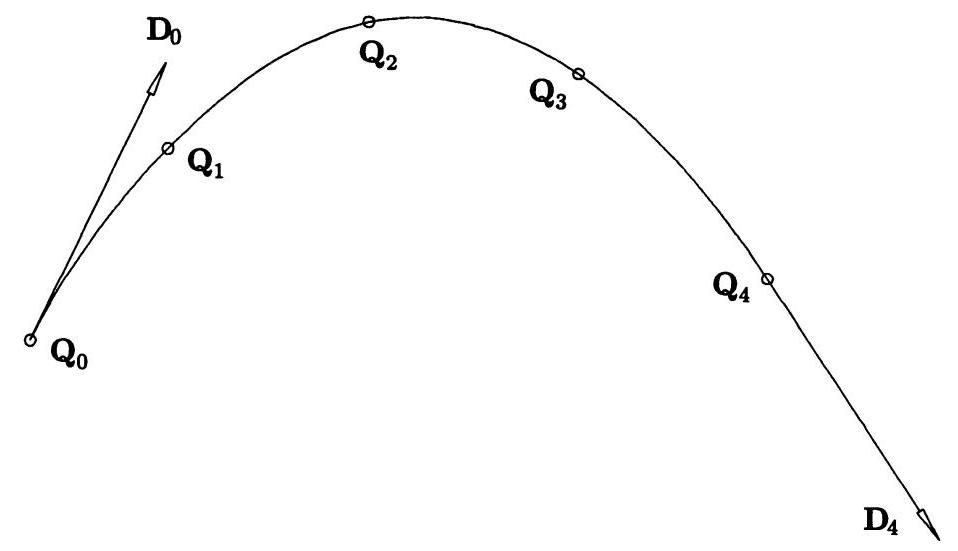
\includegraphics[max width=0.8\textwidth]{images/0193ba0d-ab19-7138-9798-cb281ce60de0_369_282_256_958_551_0.jpg}
\end{center}
\hspace*{3em} 

图 9.1. 一条插值五个点和两个端导数的曲线。

拟合中有许多微妙之处，实际上已有数百篇论文讨论这一主题。许多技术是启发式的，通常没有唯一或明确的“正确”答案。一个根本问题是，给定的数据从未指定唯一解。存在无限多条 NURBS 曲线可以插值图 9.1 中的七个数据项，或近似图 9.2 中的 \(m + 1\) 项。实施拟合算法的开发者常常被使用软件的设计师告知:“但这不是我想要的曲线！”而回复通常是:“好吧，这在数学上是正确的；它满足你给我的数据！”

拟合问题的输入通常由几何数据组成，例如点和导数。输出是 NURBS 曲线或曲面，即控制点、节点和权重。此外，必须输入度 \(p\) (或曲面的 (p, q))，或者算法必须选择一个合适的度。如果希望曲线具有 \({C}^{r}\) 连续性，则所选的度 \(p\) 必须满足

\[
p \geq  r + 1 \tag{9.1}
\]

\begin{center}
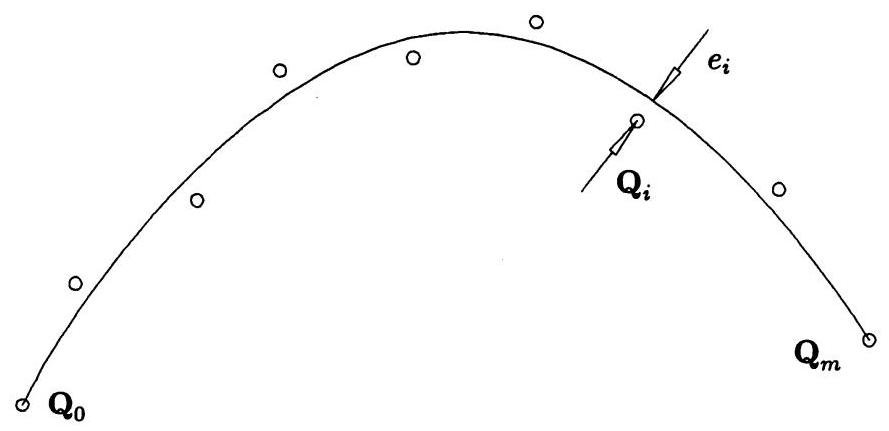
\includegraphics[max width=0.8\textwidth]{images/0193ba0d-ab19-7138-9798-cb281ce60de0_369_319_1606_889_431_0.jpg}
\end{center}
\hspace*{3em} 

图 9.2. 一条近似 \(m + 1\) 点的曲线；该曲线被约束通过端点 \({\mathbf{Q}}_{0}\) 和 \({\mathbf{Q}}_{m}\) 。

(假设没有重数为 \(> 1\) 的内部节点)。假设没有其他要求，选择 \(p = r + 1\) 通常足以进行插值。对于逼近，选择 \(p > r + 1\) 可能会产生更好的结果。例如，假设我们想要一个 \({C}^{1}\) 连续曲线来逼近表示三维空间中扭曲曲线的点数据。使用三次曲线可能会产生比二次曲线更少的控制点，尽管二次曲线能提供所需的连续性。关于在拟合过程中设置权重的文献非常少。通常，所有权重都简单地设置为 1。实际上，对于插值，可能没有理由去做其他选择(一个例外是使用分段圆弧拟合时 [Hosc92b])。对于逼近，允许权重为任意值应该会产生具有更少控制点的曲线和曲面；我们提出了一种这样的算法。最后，有许多选择节点的方法，其中大多数是启发式的。

大多数拟合算法可以分为两类:全局算法或局部算法。全局算法通过建立和求解方程组或优化问题来进行。如果给定的数据仅包含点和导数，并且控制点是唯一的未知数(度数、节点和权重已被预先选择)，那么系统是线性的，因此容易求解。如果给定了更复杂的数据，例如曲率，或者节点和/或权重也是系统未知数，那么得到的系统就是非线性的。从理论上讲，任何一个输入数据项的扰动都可以改变整个曲线或表面的形状；然而，变化的幅度随着与受影响数据项的距离增加而减小。局部算法在本质上更具几何特征，逐段构建曲线或表面，仅使用每一步的局部数据。数据项的扰动仅在局部改变曲线或表面。这些算法通常比全局方法计算成本更低。它们也能更好地处理尖点、直线段和其他局部数据异常。然而，在段边界实现期望的连续性水平更为棘手，局部方法通常导致多个内部节点。

在后续章节中，我们将介绍多种全局和局部的曲线和表面插值与逼近方法。这些方法因其经过验证的实用性而被选中，并且它们代表了广泛的技术交叉。我们强调，本章不涉及交互式曲线和表面设计，尽管这里涵盖的许多技术适用于该主题。在 NURBS 框架中的交互式设计通常采用以下一种(或两种)方法:

\begin{itemize}
\item 给定一个 NURBS 曲线或表面，通过修改权重和/或控制点交互式地改变其形状；这些技术在第 11 章中进行了讨论；
\end{itemize}

\begin{itemize}
\item 交互式构建 NURBS 曲线或曲面。局部拟合技术特别适合此任务。可以单独构建和塑造任何类型的多项式或有理段(例如，Hermite，Bézier)。除了局部控制外，一些方法还提供全局控制，例如全局张力参数。无论采用何种方法，如果结果是分段多项式或有理曲线或曲面，通常可以在最后一步转换为 NURBS 形式。
\end{itemize}


\section{全局插值}
在本节中，我们提出了将曲线插值到点和导数数据的方法，以及将曲面插值到点数据的方法。

\subsection{针对点数据的全局曲线插值}%TODO::将曲线插值到点数据
假设我们给定一组点 \(\left\{  {\mathbf{Q}}_{k}\right\}  ,k = 0,\ldots ,n\) ，并希望用一个 \(p\) 次非有理 B 样条曲线来插值这些点。如果我们为每个 \({\mathbf{Q}}_{k}\) 分配一个参数值 \({\bar{u}}_{k}\) ，并选择一个合适的节点向量 \(U = \left\{  {{u}_{0},\ldots ,{u}_{m}}\right\}\) ，我们可以建立 \(\left( {n + 1}\right)  \times  \left( {n + 1}\right)\) 个线性方程组。

\[
{\mathbf{Q}}_{k} = \mathbf{C}\left( {\bar{u}}_{k}\right)  = \mathop{\sum }\limits_{{i = 0}}^{n}{N}_{i,p}\left( {\bar{u}}_{k}\right) {\mathbf{P}}_{i} \tag{9.2}
\]

控制点 \({\mathbf{P}}_{i}\) 是 \(n + 1\) 个未知数。设 \(r\) 为 \({\mathbf{Q}}_{k}\) 中的坐标数(通常为 2、3 或 4)。请注意，这种方法与 \(r\) 无关；方程 (9.2) 有一个系数矩阵，具有 \(r\) 个右侧，并且相应地，对于 \({\mathbf{P}}_{i}\) 的 \(r\) 个坐标有 \(r\) 个解集。

选择 \({\bar{u}}_{k}\) 和 \(U\) 的问题仍然存在，它们的选择会影响曲线的形状和参数化。在本节中，我们假设参数位于范围 \(u \in  \left\lbrack  {0,1}\right\rbrack\) 内。选择 \({\bar{u}}_{k}\) 的三种常见方法是:

\begin{itemize}
\item 等距分布:
\end{itemize}

\[
{\bar{u}}_{0} = 0\;{\bar{u}}_{n} = 1
\]

\[
{\bar{u}}_{k} = \frac{k}{n}\;k = 1,\ldots ,n - 1 \tag{9.3}
\]

这种方法不推荐使用，因为当数据不均匀分布时，它可能会产生不规则的形状(例如环)。

\begin{itemize}
\item 弦长:设 \(d\) 为总弦长
\end{itemize}

\[
d = \mathop{\sum }\limits_{{k = 1}}^{n}\left| {{\mathbf{Q}}_{k} - {\mathbf{Q}}_{k - 1}}\right|  \tag{9.4}
\]

然后

\[
{\bar{u}}_{0} = 0\;{\bar{u}}_{n} = 1
\]

\[
{\bar{u}}_{k} = {\bar{u}}_{k - 1} + \frac{\left| {\mathbf{Q}}_{k} - {\mathbf{Q}}_{k - 1}\right| }{d}\;k = 1,\ldots ,n - 1 \tag{9.5}
\]

这是最广泛使用的方法，通常是足够的。它还为曲线提供了“良好”的参数化，意味着它近似于均匀参数化。

\begin{itemize}
\item 向心法:设
\end{itemize}

\[
d = \mathop{\sum }\limits_{{k = 1}}^{n}\sqrt{\left| {\mathbf{Q}}_{k} - {\mathbf{Q}}_{k - 1}\right| }
\]

然后 \({\bar{u}}_{0} = 0\;{\bar{u}}_{n} = 1\)

\[
{\bar{u}}_{k} = {\bar{u}}_{k - 1} + \frac{\sqrt{\left| {\mathbf{Q}}_{k} - {\mathbf{Q}}_{k - 1}\right| }}{d}\;k = 1,\ldots ,n - 1 \tag{9.6}
\]

这是一种较新的方法(见 [Lee89])，在数据发生急剧转弯时，它比弦长法提供更好的结果。

节点可以均匀分布，即，

\[
{u}_{0} = \cdots  = {u}_{p} = 0\;{u}_{m - p} = \cdots  = {u}_{m} = 1
\]

\[
{u}_{j + p} = \frac{j}{n - p + 1}\;j = 1,\ldots ,n - p \tag{9.7}
\]

然而，这种方法不推荐使用；如果与方程 (9.5) 或 (9.6) 一起使用，可能会导致奇异的方程组(方程 [9.2])。我们推荐以下平均技术

\[
{u}_{0} = \cdots  = {u}_{p} = 0\;{u}_{m - p} = \cdots  = {u}_{m} = 1
\]

\[
{u}_{j + p} = \frac{1}{p}\mathop{\sum }\limits_{{i = j}}^{{j + p - 1}}{\bar{u}}_{i}\;j = 1,\ldots ,n - p \tag{9.8}
\]

使用这种方法，节点反映了 \({\bar{u}}_{k}\) 的分布。此外，使用方程 (9.8) 结合方程 (9.5) 或 (9.6) 来计算 \({\bar{u}}_{k}\) 会导致一个系统(方程 [9.2])，该系统是完全正的并且带状，半带宽小于 \(p\) (见 [DeBo78])，即，如果 \(\left| {i - k}\right|  \geq  p\) 。因此，可以通过高斯消元法无需主元进行求解。

图 9.3 显示了控制点、参数和插值七个点的三次曲线的节点向量。参数通过弦长法选择，节点通过平均参数获得(公式 [9.8])。在图 9.4 中，展示了不同参数化的比较。图 9.5 显示了使用更“分散”的数据点进行的相同比较。在这两种情况下，三次曲线都通过七个点，使用均匀参数和均匀节点(实线曲线和顶部节点向量 - 参见公式 [9.3] 和 [9.7])；弦长参数和通过平均获得的节点(虚线曲线和中间节点向量 - 参见公式 [9.5] 和 [9.8])；以及通过平均获得的向心参数和节点(点划线曲线和底部节点向量 - 参见公式 [9.6] 和 [9.8])。在图 9.5 中，请注意弦长和向心参数化曲线如何适应点间距的变化。

\begin{center}
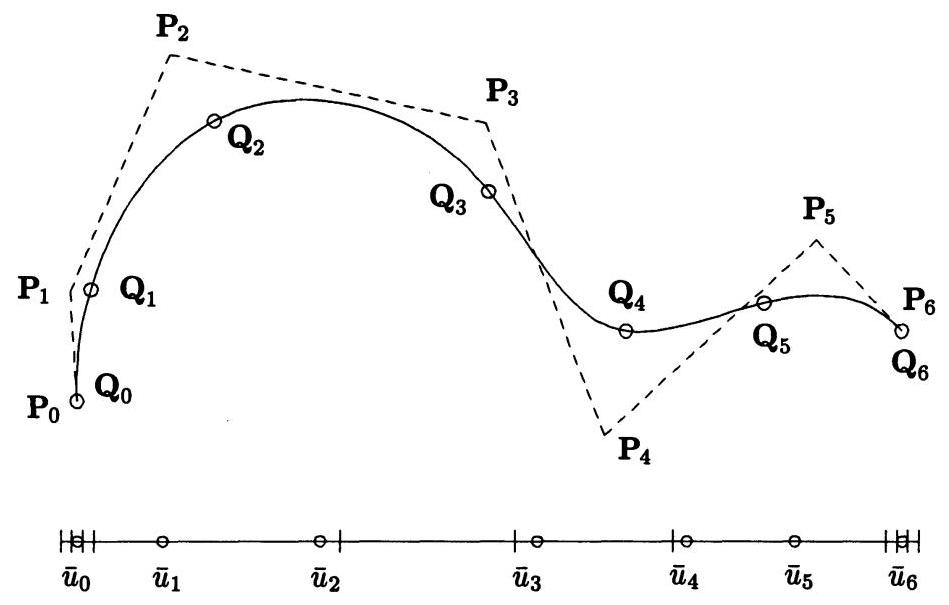
\includegraphics[max width=0.8\textwidth]{images/0193ba0d-ab19-7138-9798-cb281ce60de0_373_287_255_949_605_0.jpg}
\end{center}
\hspace*{3em} 

图 9.3. 使用弦长参数化和通过平均参数获得的节点向量的曲线插值示例。

节点向量 - 参见公式 [9.5] 和 [9.8])；以及通过平均获得的向心参数和节点(点划线曲线和底部节点向量 - 参见公式 [9.6] 和 [9.8])。在图 9.5 中，请注意弦长和向心参数化曲线如何适应点间距的变化。

\begin{center}
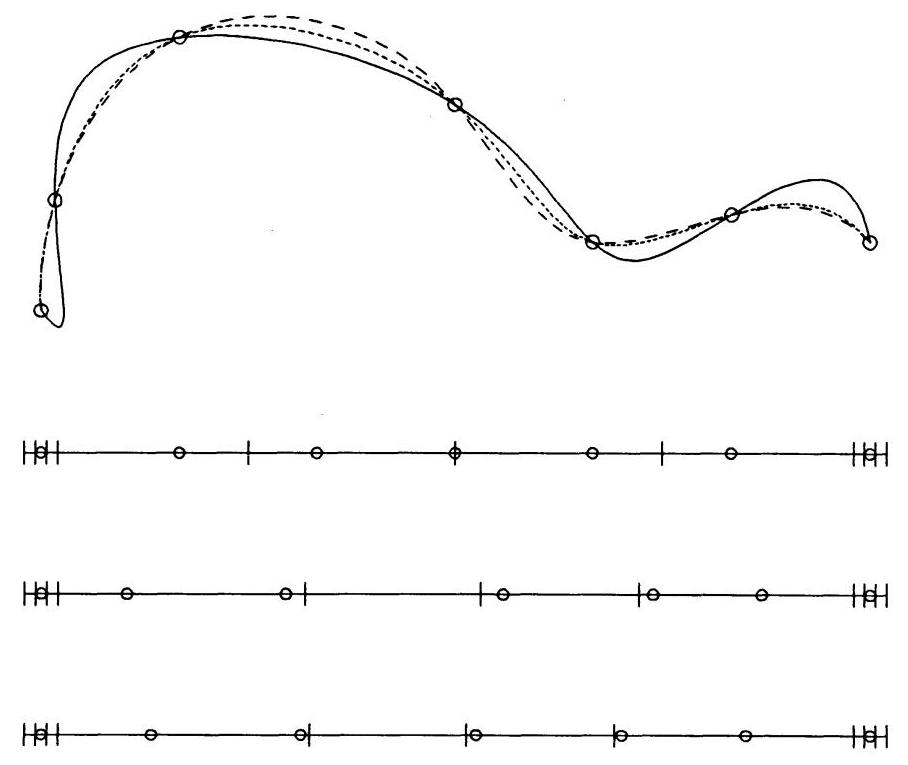
\includegraphics[max width=0.8\textwidth]{images/0193ba0d-ab19-7138-9798-cb281ce60de0_373_315_1292_908_765_0.jpg}
\end{center}
\hspace*{3em} 

图 9.4. 使用不同参数化和节点向量的曲线插值示例。

\begin{center}
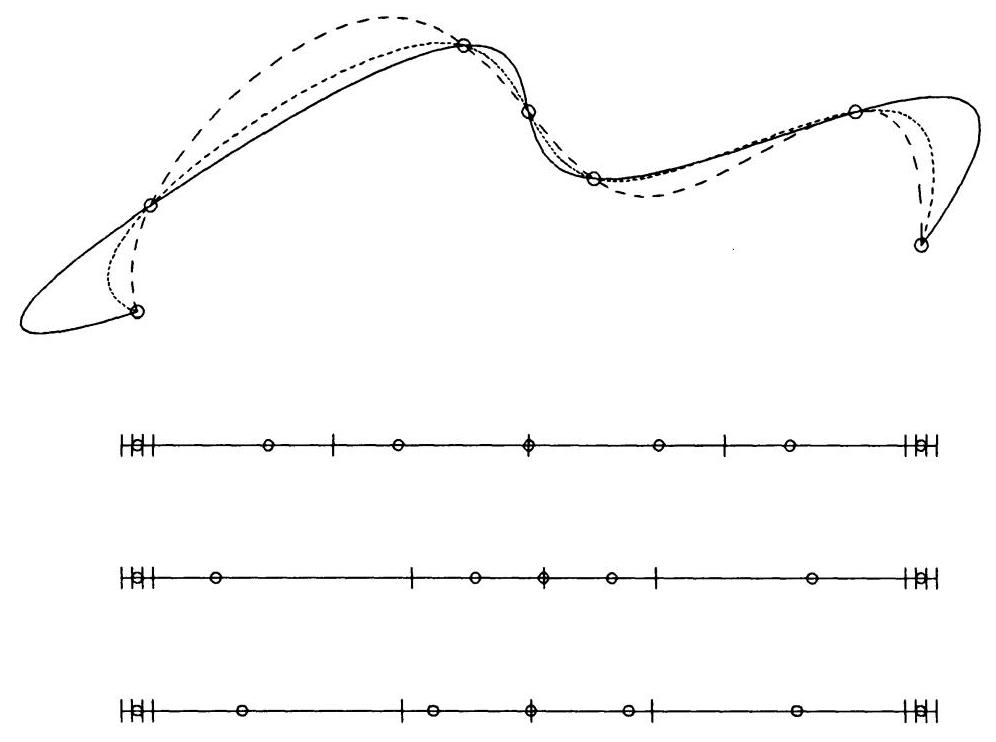
\includegraphics[max width=0.9\textwidth]{images/0193ba0d-ab19-7138-9798-cb281ce60de0_374_276_250_996_742_0.jpg}
\end{center}
\hspace*{3em} 

图 9.5. 使用不同参数化和节点向量的曲线插值示例。

图 9.6 说明了不同阶数的插值；实线、虚线和点划线曲线的阶数分别为 2、3 和 4。图 9.7 显示了全局插值器无法处理共线点集的情况。

一旦计算出 \({\bar{u}}_{k}\) 和节点，系统的 \(\left( {n + 1}\right)  \times  \left( {n + 1}\right)\) 系数矩阵(公式 [9.2])通过在每个 \({\bar{u}}_{k},k = 0,\ldots ,n\) 处评估非零基函数来建立；使用算法 A2.1 和 A2.2。

\section*{示例}

Ex9.1 设 \(\left\{  {\mathbf{Q}}_{k}\right\}   = \{ \left( {0,0}\right) ,\left( {3,4}\right) ,\left( {-1,4}\right) ,\left( {-4,0}\right) ,\left( {-4, - 3}\right) \}\) ，并假设我们希望用三次曲线插值 \({\mathbf{Q}}_{k}\) 。我们使用方程 (9.5) 和 (9.8) 来计算 \({\bar{u}}_{k}\) 和 \({u}_{j}\) ，然后建立线性方程组，方程 (9.2)。各个弦长为

\[
\left| {{\mathbf{Q}}_{1} - {\mathbf{Q}}_{0}}\right|  = 5\;\left| {{\mathbf{Q}}_{2} - {\mathbf{Q}}_{1}}\right|  = 4\;\left| {{\mathbf{Q}}_{3} - {\mathbf{Q}}_{2}}\right|  = 5\;\left| {{\mathbf{Q}}_{4} - {\mathbf{Q}}_{3}}\right|  = 3
\]

总弦长为 \(d = {17}\) 。因此

\[
{\bar{u}}_{0} = 0\;{\bar{u}}_{1} = \frac{5}{17}\;{\bar{u}}_{2} = \frac{9}{17}\;{\bar{u}}_{3} = \frac{14}{17}\;{\bar{u}}_{4} = 1
\]

使用方程 (9.8)

\[
{u}_{4} = \frac{1}{3}\left( {\frac{5}{17} + \frac{9}{17} + \frac{14}{17}}\right)  = \frac{28}{51}
\]

368 曲线与曲面拟合

\begin{center}
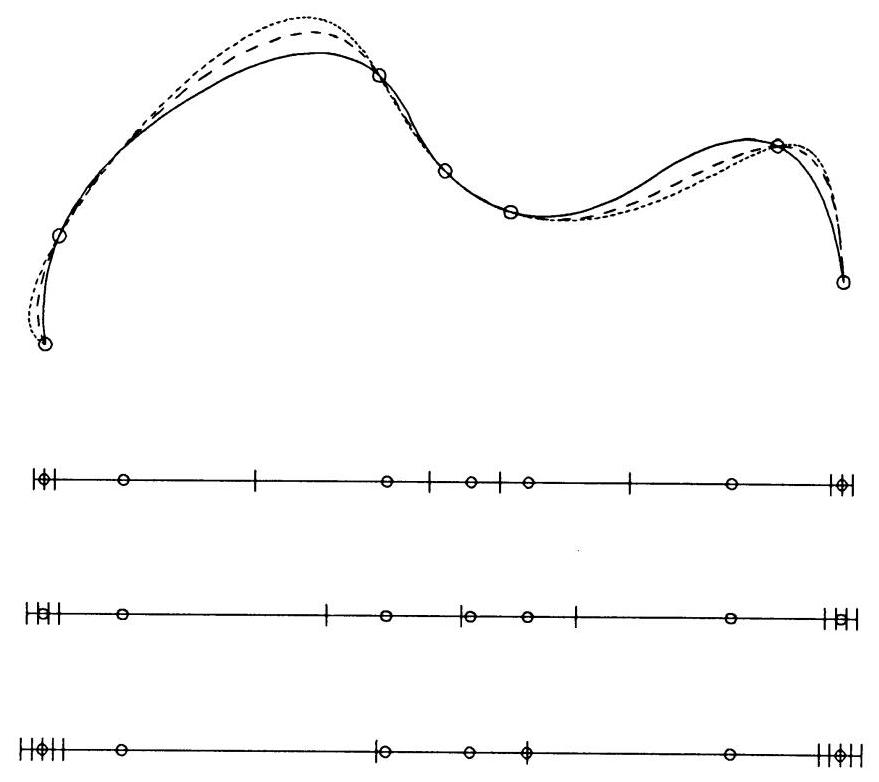
\includegraphics[max width=0.8\textwidth]{images/0193ba0d-ab19-7138-9798-cb281ce60de0_375_330_255_879_782_0.jpg}
\end{center}
\hspace*{3em} 

图 9.6. 使用弦长参数化和通过平均获得的节点进行不同度数的曲线插值。

因此

\[
U = \left\{  {0,0,0,0,\frac{28}{51},1,1,1,1}\right\}
\]

线性方程组为

\[
\left\lbrack  \begin{matrix} 1 & 0 & 0 & 0 & 0 \\  {N}_{0,3}\left( \frac{5}{17}\right) & {N}_{1,3}\left( \frac{5}{17}\right) & {N}_{2,3}\left( \frac{5}{17}\right) & {N}_{3,3}\left( \frac{5}{17}\right) & 0 \\  {N}_{0,3}\left( \frac{9}{17}\right) & {N}_{1,3}\left( \frac{9}{17}\right) & {N}_{2,3}\left( \frac{9}{17}\right) & {N}_{3,3}\left( \frac{9}{17}\right) & 0 \\  0 & {N}_{1,3}\left( \frac{14}{17}\right) & {N}_{2,3}\left( \frac{14}{17}\right) & {N}_{3,3}\left( \frac{14}{17}\right) & {N}_{4,3}\left( \frac{14}{17}\right) \\  0 & 0 & 0 & 0 & 0 \end{matrix}\right\rbrack  \left\lbrack  \begin{matrix} {\mathbf{P}}_{0} \\  {\mathbf{P}}_{1} \\  {\mathbf{P}}_{2} \\  {\mathbf{P}}_{3} \\  {\mathbf{P}}_{4} \end{matrix}\right\rbrack
\]

\[
= \left\lbrack  \begin{array}{l} {\mathbf{Q}}_{0} \\  {\mathbf{Q}}_{1} \\  {\mathbf{Q}}_{2} \\  {\mathbf{Q}}_{3} \\  {\mathbf{Q}}_{4} \end{array}\right\rbrack
\]

\begin{center}
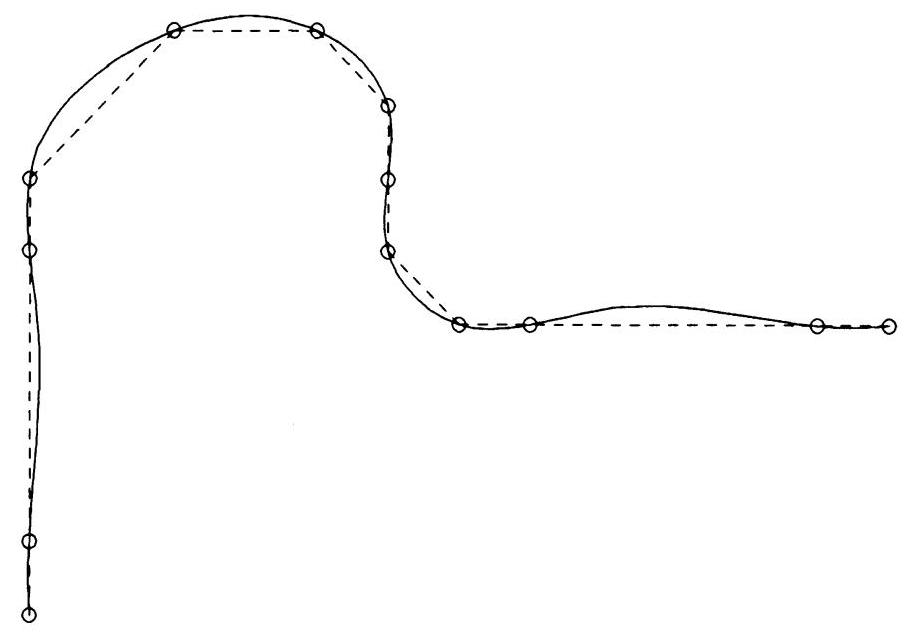
\includegraphics[max width=0.8\textwidth]{images/0193ba0d-ab19-7138-9798-cb281ce60de0_376_313_250_914_637_0.jpg}
\end{center}
\hspace*{3em} 

图 9.7. 对包含共线点的数据进行全局三次曲线插值(见虚线)。

现在我们总结全局插值算法。我们假设有两个实用程序来解决线性方程组:

\begin{itemize}
\item LUDecomposition(A, q, sbw) 用于将 \(q \times  q\) 系数矩阵分解为下三角和上三角组件，半带宽为 sbw；为简单起见，我们假设 \(\mathrm{A}\) 是一个 \(q \times  q\) 方阵，但应使用一个只存储非零带的实用程序；
\end{itemize}

\begin{itemize}
\item ForwardBackward(A, q, sbw, rhs, sol) 用于执行前向/后向替代(见 [Pres88])； rhs [] 是系统的右侧( \({\mathbf{Q}}_{k}\) 的坐标)，而 sol [] 是解向量( \({\mathbf{P}}_{i}\) 的坐标)。
\end{itemize}

该算法还利用了第2章中的 FindSpan( ) 和 BasisFuns( )。

\HRule

ALGORITHM A9.1

\hspace*{1em} \(\texttt{GlobalCurveInterp}\left( {n,Q,r,p,m,U,P}\right)\)

\hspace*{3em} \{ /* Global interpolation through \(n + 1\) points */

\hspace*{4em} /* Input: n, Q, r, p */

\hspace*{4em} /* Output: m, U, P */

\hspace*{2em} m = n+p+1;

\hspace*{3em} Compute the uk; /* Eq. (9.5) or (9.6) */

\hspace*{3em} Compute the knot vector \(U\) ; \(\;/ *\) Eq. (9.8) \(*\) /

\hspace*{3em} Initialize array A to zero;

\hspace*{2em} for (i = 0; i<=n; i++)

\hspace*{4em} \{ /* Set up coefficient matrix */

\hspace*{4em} span = FindSpan(n, p, uk[i], U);

\hspace*{4em} BasisFuns(span, uk[i], p, U, A[i][span-p]); /* Get ith row */

\hspace*{4em} \}

LUDecomposition \(\left( {A,n + 1,p - 1}\right)\) ;

for (i=0; i<r; i++) /*r is the number of coordinates */

\hspace*{1em} \{

\hspace*{1em} for \(\left( {j = 0;j <  = n;j +  + }\right) \;\) rhs \(\left\lbrack  j\right\rbrack   =\) ith coordinate of \(Q\left\lbrack  j\right\rbrack\) ;

\hspace*{1em} ForwardBackward(A, n+1, p-1, rhs, sol);

\hspace*{1em} for \(\left( {j = 0;j <  = n;j +  + }\right) \;\) ith coordinate of \(P\left\lbrack  j\right\rbrack   = \operatorname{sol}\left\lbrack  j\right\rbrack\) ;

\hspace*{1em} \}

\}

\HRule



\subsection{指定端导数的全局曲线插值}

指定导数向量作为输入数据并不罕见。在这种情况下，求解过程类似于算法 A9.1:

1. 计算与点 \({\mathbf{Q}}_{k}\) 对应的参数 \({\bar{u}}_{k}\) ；

2. 计算节点向量 \(U\) ；

3. 评估基函数以建立线性方程组，以控制点作为未知数；

4. 求解该系统。

只有步骤 2 和 3 与前一种情况略有不同。每个导数产生一个额外的节点和控制点，因此产生一个额外的线性方程。使用第2章和第3章的导数公式来建立额外的方程，例如，方程 (2.7)、(2.10) 和 (3.3)-(3.10)。我们现在用一阶导数的示例来说明这一点。

设 \(\left\{  {\mathbf{Q}}_{k}\right\}  ,k = 0,\ldots ,n\) 为点，并假设 \({\mathbf{D}}_{0}\) 和 \({\mathbf{D}}_{n}\) 分别是曲线起点和终点的一阶导数向量。我们希望用一个 \(p\) 次曲线来插值这些数据。

\[
\mathbf{C}\left( u\right)  = \mathop{\sum }\limits_{{i = 0}}^{{n + 2}}{N}_{i,p}\left( u\right) {\mathbf{P}}_{i}
\]

如前所述，使用方程 (9.5) 或方程 (9.6) 计算 \({\bar{u}}_{k},k = 0,\ldots ,n\) 。然后设置 \(m = n + p + 3\) 并通过以下方式获得 \(m + 1\) 节点:

\[
{u}_{0} = \cdots  = {u}_{p} = 0\;{u}_{m - p} = \cdots  = {u}_{m} = 1
\]

\[
{u}_{j + p + 1} = \frac{1}{p}\mathop{\sum }\limits_{{i = j}}^{{j + p - 1}}{\bar{u}}_{i}\;j = 0,\ldots ,n - p + 1 \tag{9.9}
\]

注意，方程 (9.9) 类似于方程 (9.8)，只是我们通过将 \(j\) 从 0 运行到 \(n - p + 1\) 来获得两个额外的节点。如前所述，方程 (9.2) 产生 \(n + 1\) 个方程。

\[
{\mathbf{Q}}_{k} = \mathbf{C}\left( {\bar{u}}_{k}\right)  = \mathop{\sum }\limits_{{i = 0}}^{{n + 2}}{N}_{i,p}\left( {\bar{u}}_{k}\right) {\mathbf{P}}_{i} \tag{9.10}
\]

方程 (3.7) 产生两个额外的方程，即

\[
- {\mathbf{P}}_{0} + {\mathbf{P}}_{1} = \frac{{u}_{p + 1}}{p}{\mathbf{D}}_{0} \tag{9.11}
\]

\[
- {\mathbf{P}}_{n + 1} + {\mathbf{P}}_{n + 2} = \frac{1 - {u}_{m - p - 1}}{p}{\mathbf{D}}_{n} \tag{9.12}
\]

将方程 (9.11) 和 (9.12) 作为第二个和倒数第二个方程插入方程 (9.10)，得到一个 \(\left( {n + 3}\right)  \times  \left( {n + 3}\right)\) 带状线性系统。图 9.8 显示了具有指定端切线的三次曲线插值。导数的小、中、大幅度分别产生实线、虚线和点线。图 9.9 说明了对相同数据点的插值，但具有不同的端切线方向和导数幅度。


\subsection{三次样条曲线插值}

之前的方法(方程 [9.9]-[9.12])适用于任何阶数 \(p > 1\) 。如果 \(p = 3\) ，则存在一种更高效的算法，产生传统的 \({C}^{2}\) 三次样条。 \({\bar{u}}_{k}\) 的计算与之前相同。节点是

\[
{u}_{0} = \cdots  = {u}_{3} = 0\;{u}_{n + 3} = \cdots  = {u}_{n + 6} = 1
\]

\[
{u}_{j + 3} = {\bar{u}}_{j}\;j = 1,\ldots ,n - 1 \tag{9.13}
\]

换句话说， \({\mathbf{Q}}_{k}\) 的插值发生在节点处。前两个和最后两个方程分别为

\[
{\mathbf{P}}_{0} = {\mathbf{Q}}_{0}
\]

\[
- {\mathbf{P}}_{0} + {\mathbf{P}}_{1} = \frac{{u}_{4}}{3}{\mathbf{D}}_{0} \tag{9.14}
\]

372 曲线与曲面拟合

\begin{center}
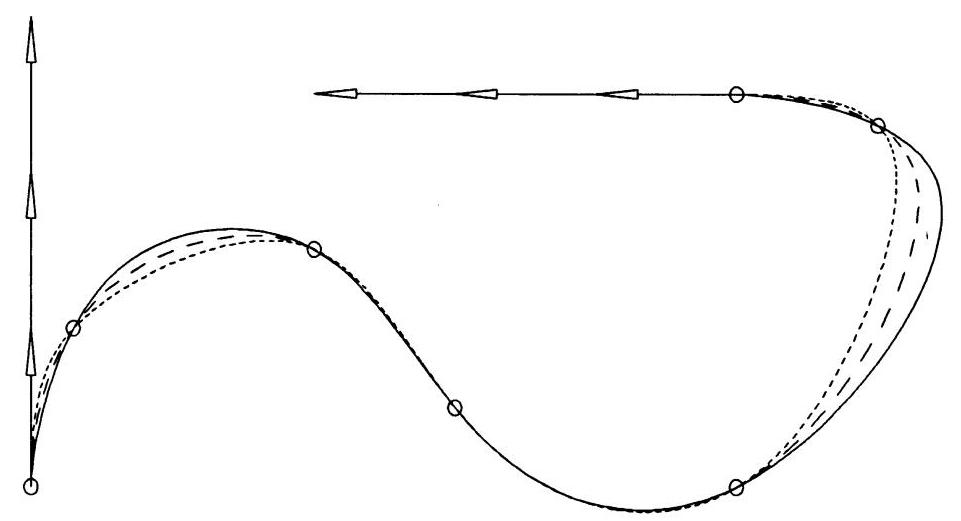
\includegraphics[max width=0.8\textwidth]{images/0193ba0d-ab19-7138-9798-cb281ce60de0_378_284_1578_961_521_0.jpg}
\end{center}
\hspace*{3em} 

图 9.8. 具有不同端导数幅度的全局三次曲线插值。

\begin{center}
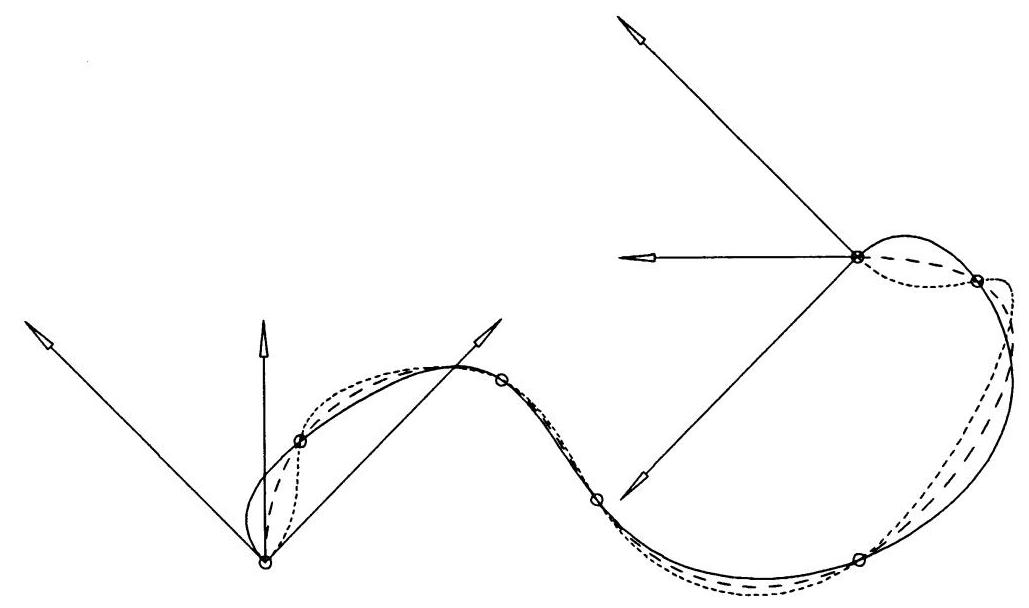
\includegraphics[max width=0.9\textwidth]{images/0193ba0d-ab19-7138-9798-cb281ce60de0_379_244_251_1029_608_0.jpg}
\end{center}
\hspace*{3em} 

图 9.9. 具有不同端导数方向的全局三次曲线插值。

和

\[
- {\mathbf{P}}_{n + 1} + {\mathbf{P}}_{n + 2} = \frac{1 - {u}_{n + 2}}{3}{\mathbf{D}}_{n}
\]

\[
{\mathbf{P}}_{n + 2} = {\mathbf{Q}}_{n} \tag{9.15}
\]

这些可以直接求解。回想一下，在一个内部节点只有三个非零的三次基函数，其余的 \(n - 1\) 方程具有以下形式

\[
{\mathbf{Q}}_{k} = \mathbf{C}\left( {\bar{u}}_{k}\right)  = {N}_{k,3}\left( {\bar{u}}_{k}\right) {\mathbf{P}}_{k} + {N}_{k + 1,3}\left( {\bar{u}}_{k}\right) {\mathbf{P}}_{k + 1} + {N}_{k + 2,3}\left( {\bar{u}}_{k}\right) {\mathbf{P}}_{k + 2} \tag{9.16}
\]

对于 \(k = 1,\ldots ,n - 1\) 。设定

\[
{a}_{k} = {N}_{k,3}\left( {\bar{u}}_{k}\right) \;{b}_{k} = {N}_{k + 1,3}\left( {\bar{u}}_{k}\right) \;{c}_{k} = {N}_{k + 2,3}\left( {\bar{u}}_{k}\right)
\]

产生三对角系统

\[
\left\lbrack  \begin{matrix} {\mathbf{R}}_{2} \\  {\mathbf{R}}_{3} \\  \vdots \\  {\mathbf{R}}_{n - 1} \\  {\mathbf{R}}_{n} \end{matrix}\right\rbrack   = \left\lbrack  \begin{matrix} {\mathbf{Q}}_{1} - {a}_{1}{\mathbf{P}}_{1} \\  {\mathbf{Q}}_{2} \\  \vdots \\  {\mathbf{Q}}_{n - 2} \\  {\mathbf{Q}}_{n - 1} - {c}_{n - 1}{\mathbf{P}}_{n + 1} \end{matrix}\right\rbrack
\]

\[
= \left\lbrack  \begin{matrix} {b}_{1} & {c}_{1} & 0 & \cdots & 0 & 0 & 0 \\  {a}_{2} & {b}_{2} & {c}_{2} & \cdots & 0 & 0 & 0 \\  \vdots & \vdots & \vdots &  \ddots  & \vdots & \vdots & \vdots \\  0 & 0 & 0 & \cdots & {a}_{n - 2} & {b}_{n - 2} & {c}_{n - 2} \\  0 & 0 & 0 & \cdots & 0 & {a}_{n - 1} & {b}_{n - 1} \end{matrix}\right\rbrack  \left\lbrack  \begin{matrix} {\mathbf{P}}_{2} \\  {\mathbf{P}}_{3} \\  \vdots \\  {\mathbf{P}}_{n - 1} \\  {\mathbf{P}}_{n} \end{matrix}\right\rbrack   \tag{9.17}
\]

该系统可以通过一个简单的算法来解决，该算法实时计算方程 (9.17) 中矩阵的行。它需要两个长度为 \(n + 1\) 的局部数组 R[] 和 dd[]，以及一个长度为 4 的数组 abc[]，该数组存储 \({a}_{k},{b}_{k},{c}_{k},0\) 。它假设 \({\mathbf{P}}_{0},{\mathbf{P}}_{1},{\mathbf{P}}_{n + 1},{\mathbf{P}}_{n + 2}\) 已经计算并加载到数组 \(\mathbf{P}\) 中。该算法可以适应处理具有任意数量坐标的点。

算法 A9.2

\HRule

SolveTridiagonal(n, Q, U, P)

\hspace*{2em} \{ /* Solve tridiagonal system for C2 cubic spline */

\hspace*{6em} /* Input: n, Q, U, P[0], P[1], P[n+1], P[n+2] */

\hspace*{6em} /* Output: P */

\hspace*{2em} for (i=3; i<n; i++) R[i] = Q[i-1];

\hspace*{2em} BasisFuns(4, U[4],3, U, abc);

\hspace*{2em} den = abc[1];

\hspace*{2em} P[2] = (Q[1]-abc[0]*P[1])/den;

\hspace*{2em} for (i=3; i<n; i++)

\hspace*{5em} \{

\hspace*{5em} dd[i] = abc[2]/den;

\hspace*{5em} BasisFuns(i+2, U[i+2],3, U, abc);

\hspace*{5em} den = abc[1]-abc[0]*dd[i];

\hspace*{5em} \(P\left\lbrack  i\right\rbrack   = \left( {R\left\lbrack  i\right\rbrack   - {abc}\left\lbrack  0\right\rbrack   * P\left\lbrack  {i - 1}\right\rbrack  }\right) /{den};\)

\hspace*{4em} \}

\hspace*{2em} dd[n] = abc[2]/den;

\hspace*{2em} BasisFuns(n+2, U[n+2],3, U, abc);

\hspace*{2em} den \(= {abc}\left\lbrack  1\right\rbrack   - {abc}\left\lbrack  0\right\rbrack   * {dd}\left\lbrack  n\right\rbrack\) ;

\hspace*{2em} \(P\left\lbrack  n\right\rbrack   = \left( {Q\left\lbrack  {n - 1}\right\rbrack   - {abc}\left\lbrack  2\right\rbrack   * P\left\lbrack  {n + 1}\right\rbrack   - {abc}\left\lbrack  0\right\rbrack   * P\left\lbrack  {n - 1}\right\rbrack  }\right) /{den};\)

\hspace*{2em} for (i=n-1; i>=2; i--) P[i] = P[i]-dd[i+1]*P[i+1];

\hspace*{2em} \}

\HRule

图 9.10 显示了使用该三次样条算法插值的数据。

通常，仅指定导数向量的切向方向而不指定大小。我们用 \({\mathbf{T}}_{0}\) 和 \({\mathbf{T}}_{n}\) 表示单位长度的切向量。在这种情况下，必须估计大小 \({\alpha }_{0}\) 和 \({\alpha }_{n}\) 。设定

\[
{\mathbf{D}}_{0} = {\alpha }_{0}{\mathbf{T}}_{0}\;{\mathbf{D}}_{n} = {\alpha }_{n}{\mathbf{T}}_{n} \tag{9.18}
\]

并按之前的方式进行。一个合理的选择是将 \({\alpha }_{0}\) 和 \({\alpha }_{n}\) 设置为总弦长 \(d\) ，如方程 (9.4) 中计算的那样。在交互环境中， \({\alpha }_{0}\) 和 \({\alpha }_{n}\) 可以用作额外的形状控制。



\subsection{指定一阶导数的全局曲线插值}

现在假设在每个点上给定一阶导数 \({\mathbf{D}}_{k}\) ， \({\mathbf{Q}}_{k},k =\)  \(0,\ldots ,n\) 。有 \(2\left( {n + 1}\right)\) 个数据项和同样数量的未知控制点。

\begin{center}
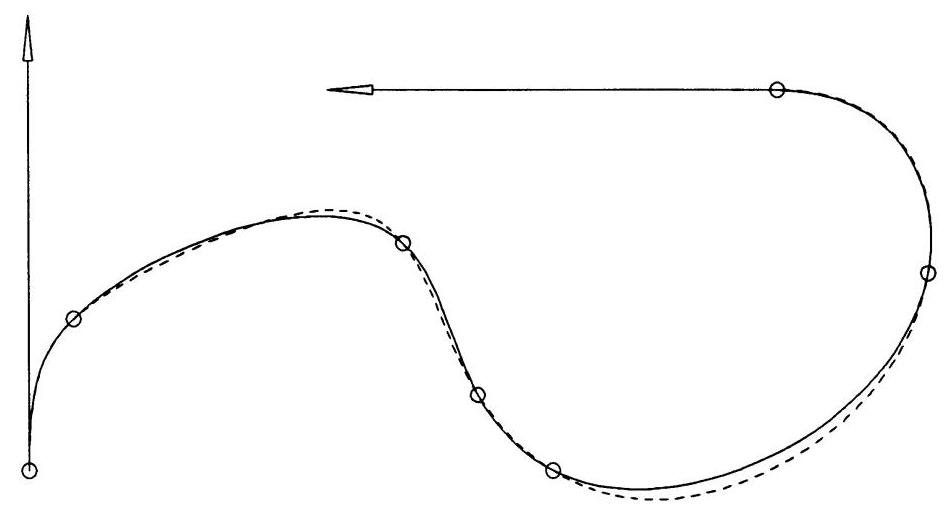
\includegraphics[max width=0.8\textwidth]{images/0193ba0d-ab19-7138-9798-cb281ce60de0_381_285_251_951_511_0.jpg}
\end{center}
\hspace*{3em} 

图 9.10。三次样条插值(实线)与通过使用弦长参数化和通过平均计算的节点获得的常规三次插值(虚线)进行比较。

表达 \({\mathbf{Q}}_{k}\) 的 \(n + 1\) 方程为

\[
{\mathbf{Q}}_{k} = \mathbf{C}\left( {\bar{u}}_{k}\right)  = \mathop{\sum }\limits_{{i = 0}}^{{{2n} + 1}}{N}_{i,p}\left( {\bar{u}}_{k}\right) {\mathbf{P}}_{i} \tag{9.19}
\]

并且从方程 (2.10) 和 (3.3) 中，表达 \({\mathbf{D}}_{k}\) 的 \(n + 1\) 方程为

\[
{\mathbf{D}}_{k} = {\mathbf{C}}^{\prime }\left( {\bar{u}}_{k}\right)  = \mathop{\sum }\limits_{{i = 0}}^{{{2n} + 1}}{N}_{i,p}^{\prime }\left( {\bar{u}}_{k}\right) {\mathbf{P}}_{i} \tag{9.20}
\]

参数 \({\bar{u}}_{k}\) 是通过公式 (9.5) 或公式 (9.6) 计算得出的。节点的数量是

\[
2\left( {n + 1}\right)  + p + 1 \tag{9.21}
\]

应该选择以反映 \({\bar{u}}_{k}\) 的分布。对于 \(p = 2\) 和 \(p = 3\) ，令人满意的选择是

\[
U = \left\{  {0,0,0,\frac{{\bar{u}}_{1}}{2},{\bar{u}}_{1},\frac{{\bar{u}}_{1} + {\bar{u}}_{2}}{2},{\bar{u}}_{2},\ldots ,{\bar{u}}_{n - 1},\frac{{\bar{u}}_{n - 1} + 1}{2},1,1,1}\right\}   \tag{9.22}
\]

和 \(\;U = \left\{  {0,0,0,0,\frac{{\bar{u}}_{1}}{2},\frac{2{\bar{u}}_{1} + {\bar{u}}_{2}}{3},\frac{{\bar{u}}_{1} + 2{\bar{u}}_{2}}{3},\ldots ,\frac{{\bar{u}}_{n - 2} + 2{\bar{u}}_{n - 1}}{3}}\right.\) ，

\[
\left. {\frac{{\bar{u}}_{n - 1} + 1}{2},1,1,1,1}\right\}   \tag{9.23}
\]

分别。方程 (9.19) 和 (9.20) 以交替的方式合并，以产生一个 \(2\left( {n + 1}\right)  \times  2\left( {n + 1}\right)\) 带状线性系统。例如，设 \(p = 3\) 。将方程 (9.23) 的第一个和最后一个内部节点表示为

\[
{u}_{4} = \frac{{\bar{u}}_{1}}{2}\;{u}_{m - p - 1} = \frac{{\bar{u}}_{n - 1} + 1}{2}
\]

方程组为

\[
{\mathbf{P}}_{0}
\]

\[
= {\mathbf{Q}}_{0}
\]

\[
- {\mathbf{P}}_{0} + {\mathbf{P}}_{1}
\]

\[
= \frac{{u}_{4}}{3}{\mathbf{D}}_{0}
\]

\[
{N}_{1,3}\left( {\bar{u}}_{1}\right) {\mathbf{P}}_{1} + \cdots  + {N}_{4,3}\left( {\bar{u}}_{1}\right) {\mathbf{P}}_{4}
\]

\[
= {\mathbf{Q}}_{1}
\]

\[
{N}_{1,3}^{\prime }\left( {\bar{u}}_{1}\right) {\mathbf{P}}_{1} + \cdots  + {N}_{4,3}^{\prime }\left( {\bar{u}}_{1}\right) {\mathbf{P}}_{4}
\]

\[
= {\mathbf{D}}_{1}
\]

\(\vdots\)

\[
{N}_{{2n} - 3,3}\left( {\bar{u}}_{n - 1}\right) {\mathbf{P}}_{{2n} - 3} + \cdots  + {N}_{{2n},3}\left( {\bar{u}}_{n - 1}\right) {\mathbf{P}}_{2n}\; = {\mathbf{Q}}_{n - 1}
\]

\[
{N}_{{2n} - 3,3}^{\prime }\left( {\bar{u}}_{n - 1}\right) {\mathbf{P}}_{{2n} - 3} + \cdots  + {N}_{{2n},3}^{\prime }\left( {\bar{u}}_{n - 1}\right) {\mathbf{P}}_{2n}\; = {\mathbf{D}}_{n - 1}
\]

\[
- {\mathbf{P}}_{2n} + {\mathbf{P}}_{{2n} + 1} = \frac{1 - {u}_{m - p - 1}}{3}{\mathbf{D}}_{n}
\]

\[
{\mathbf{P}}_{{2n} + 1} = {\mathbf{Q}}_{n} \tag{9.24}
\]

使用算法 A2.3 (DersBasisFuns (   )) 来计算 \({N}_{i,3}\left( {\bar{u}}_{k}\right)\) 和 \({N}_{i,3}^{\prime }\left( {\bar{u}}_{k}\right)\) 。

如果给定单位长度切向量 \({\mathbf{T}}_{k}\) 而不是 \({\mathbf{D}}_{k}\) ，则必须估计幅度 \({\alpha }_{k}\) 。设置所有 \({\alpha }_{k} = d\) ，其中 \(d\) 是总弦长，是一个合理的选择。图 9.11 显示了对点和导数的二次(实线)和三次(虚线)曲线插值。图 9.12 说明了通过在数据点使用不同导数幅度获得的不同曲线插值之间的比较。实线曲线应用 \({\alpha }_{k} = d\) (中间切线)；

\begin{center}
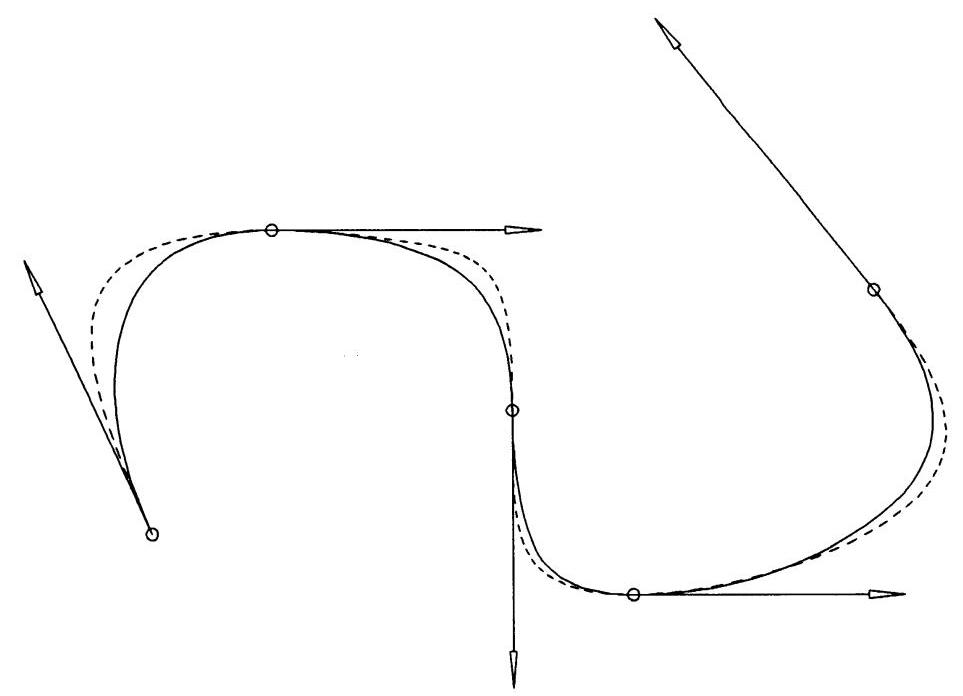
\includegraphics[max width=0.8\textwidth]{images/0193ba0d-ab19-7138-9798-cb281ce60de0_382_280_1347_963_696_0.jpg}
\end{center}
\hspace*{3em} 

图 9.11. 在每个数据点指定导数的二次(实线)和三次(虚线)曲线插值。

376 曲线和曲面拟合，虚线曲线具有 \({\alpha }_{k} = 3/{2d}\) (大切线)；点线曲线是通过 \({\alpha }_{k} = 1/{2d}\) (小切线)获得的。图 9.13 显示了对指定点和一阶导数的二次曲线插值的控制点。

\begin{center}
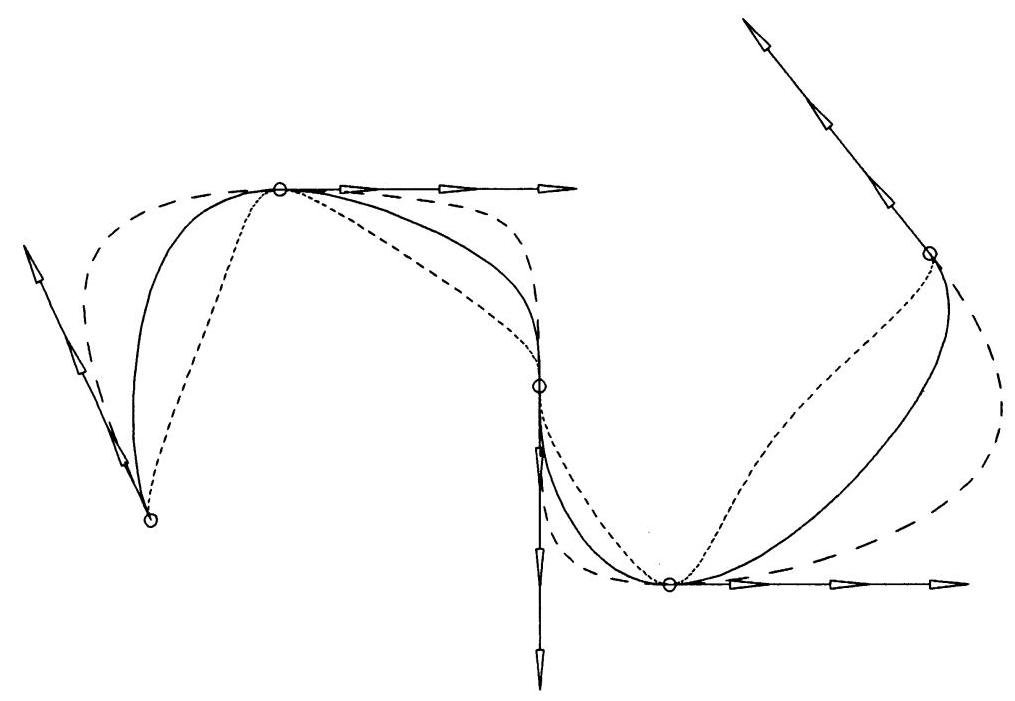
\includegraphics[max width=0.9\textwidth]{images/0193ba0d-ab19-7138-9798-cb281ce60de0_383_257_266_1015_701_0.jpg}
\end{center}
\hspace*{3em} 

图 9.12. 在每个点具有不同切向导数的三次曲线插值。



\subsection{全局曲面插值}

我们现在转向曲面的全局插值。我们给定一组 \((n +\) 1) \(\times  \left( {m + 1}\right)\) 数据点 \(\left\{  {\mathbf{Q}}_{k,\ell }\right\}  ,k = 0,\ldots ,n\) 和 \(\ell  = 0,\ldots ,m\) ，我们希望构造一个非有理的 (p, q) 次 B 样条曲面来插值这些点，即

\[
{\mathbf{Q}}_{k,\ell } = \mathbf{S}\left( {{\bar{u}}_{k},{\bar{v}}_{\ell }}\right)  = \mathop{\sum }\limits_{{i = 0}}^{n}\mathop{\sum }\limits_{{j = 0}}^{m}{N}_{i,p}\left( {\bar{u}}_{k}\right) {N}_{j,q}\left( {\bar{v}}_{\ell }\right) {\mathbf{P}}_{i,j} \tag{9.25}
\]

再次，首要任务是计算 \(\left( {{\bar{u}}_{k},{\bar{v}}_{\ell }}\right)\) 和节点向量 \(U\) 及 \(V\) 的合理值。我们展示如何计算 \({\bar{u}}_{k}\) ； \({\bar{v}}_{\ell }\) 是类似的。一个常见的方法是使用公式 (9.5) 或公式 (9.6) 来计算每个 \(\ell\) 的参数 \({\bar{u}}_{0}^{\ell },\ldots ,{\bar{u}}_{n}^{\ell }\) ，然后通过对所有 \({\bar{u}}_{k}^{\ell },\ell  = 0,\ldots ,m\) 进行平均来获得每个 \({\bar{u}}_{k}\) ，即

\[
{\bar{u}}_{k} = \frac{1}{m + 1}\mathop{\sum }\limits_{{\ell  = 0}}^{m}{\bar{u}}_{k}^{\ell }\;k = 0,\ldots ,n
\]

其中对于每个固定的 \(\ell ,{\bar{u}}_{k}^{\ell },k = 0,\ldots ,n\) ，是通过公式 (9.5) 或公式 (9.6) 计算的。以下是使用公式 (9.5) 的高效算法。它同时计算 \({\bar{u}}_{k}\) 和 \({\bar{v}}_{\ell }\) 。它需要一个长度为 \(\max \left( {n + 1,m + 1}\right)\) 的局部数组 cds [] 来存储弦长

\begin{center}
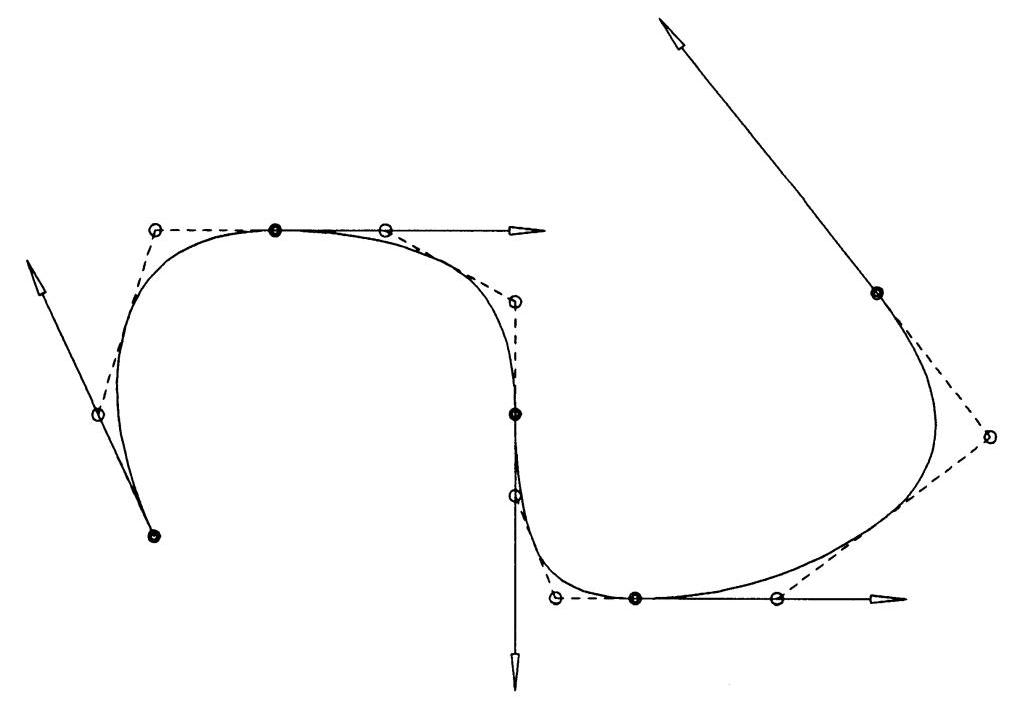
\includegraphics[max width=0.9\textwidth]{images/0193ba0d-ab19-7138-9798-cb281ce60de0_384_256_271_1010_701_0.jpg}
\end{center}
\hspace*{3em} 

图 9.13. 二次 B 样条曲线插值器的控制点，插值于具有指定导数的数据。

距离 \(\left| {{\mathbf{Q}}_{k,\ell } - {\mathbf{Q}}_{k - 1,\ell }}\right| ,k = 1,\ldots ,n\) (在 \(v\) 方向上也是如此)。函数 Distance3D( ) 计算两个三维点之间的距离。该算法处理当一行的总弦长等于零的情况，这是构造三面体表面的必要条件。

算法 A9.3

\HRule

SurfMeshParams(n, m, Q, uk, vl)

\hspace*{3em} \{ /* Compute parameters for */

\hspace*{6em} /* global surface interpolation */

\hspace*{6em} /* Input: n, m, Q */

\hspace*{6em} /* Output: uk, vl */

\hspace*{4em} /* First get the uk */

\hspace*{2em} num = m+1; /* number of nondegenerate rows */

\hspace*{2em} uk[0] = 0.0 ; ux[n] = 1.0 ;

\hspace*{2em} for \(\left( {\mathrm{k} = 1;\mathrm{k} < \mathrm{n};\mathrm{k} +  + }\right) \;\mathrm{{uk}}\left\lbrack  \mathrm{k}\right\rbrack   = {0.0}\) ;

\hspace*{2em} for (l=0; l<=m; l++)

\hspace*{5em} \{

\hspace*{5em} total \(= {0.0};\;/ *\) total chord length of row \(*\) /

\hspace*{5em} for (k=1; k<=n; k++)

\hspace*{7em} \{

\hspace*{7em} cds[k] = Distance3D(Q[k][l], Q[k-1][l]);

\hspace*{7em} total = total + cds[k];

\hspace*{7em} \}

\hspace*{5em} if (total == 0.0) num = num-1;

\hspace*{4em} else

\hspace*{5em} \{

\hspace*{5em} d = 0.0 ;

\hspace*{5em} for (k=1; k<n; k++)

\hspace*{7em} \{

\hspace*{7em} d = d + cds[k];

\hspace*{7em} \({uk}\left\lbrack  k\right\rbrack   = {uk}\left\lbrack  k\right\rbrack   + d/\) total;

\hspace*{6em} \}

\hspace*{5em} \}

\hspace*{2em} \}

if (num == 0) return(error);

for \(\left( {k = 1;k < n;k +  + }\right) \;{uk}\left\lbrack  k\right\rbrack   = {uk}\left\lbrack  k\right\rbrack  /{num}\) ;

\hspace*{3em} /* Now do the same for vl */

\}

\HRule

一旦计算出 \(\left( {{\bar{u}}_{k},{\bar{v}}_{\ell }}\right)\) ，节点向量 \(U\) 和 \(V\) 可以通过公式 (9.8) 获得。

现在进行控制点的计算。显然，方程 (9.25) 表示 \(\left( {n + 1}\right)  \times  \left( {m + 1}\right)\) 中的线性方程，未知数为 \({\mathbf{P}}_{i,j}\) 。然而，由于 \(\mathbf{S}\left( {u,v}\right)\) 是一个张量积曲面， \({\mathbf{P}}_{i,j}\) 可以更简单高效地通过一系列曲线插值获得。对于固定的 \(\ell\) ，将方程 (9.25) 写为

\[
{\mathbf{Q}}_{k,\ell } = \mathop{\sum }\limits_{{i = 0}}^{n}{N}_{i,p}\left( {\bar{u}}_{k}\right) \left( {\mathop{\sum }\limits_{{j = 0}}^{m}{N}_{j,q}\left( {\bar{v}}_{\ell }\right) {\mathbf{P}}_{i,j}}\right)  = \mathop{\sum }\limits_{{i = 0}}^{n}{N}_{i,p}\left( {\bar{u}}_{k}\right) {\mathbf{R}}_{i,\ell } \tag{9.26}
\]

其中

\[
{\mathbf{R}}_{i,\ell } = \mathop{\sum }\limits_{{j = 0}}^{m}{N}_{j,q}\left( {\bar{v}}_{\ell }\right) {\mathbf{P}}_{i,j} \tag{9.27}
\]

注意，方程 (9.26) 只是通过点 \({\mathbf{Q}}_{k,\ell },k =\)  \(0,\ldots ,n\) 的曲线插值。 \({\mathbf{R}}_{i,\ell }\) 是在固定 \(v = {\bar{v}}_{\ell }\) 的 \(\mathbf{S}\left( {u,v}\right)\) 上的等参数曲线的控制点。现在固定 \(i\) 并让 \(\ell\) 变化，方程 (9.27) 是通过点 \({\mathbf{R}}_{i,0},\ldots ,{\mathbf{R}}_{i,m}\) 的曲线插值，以 \({\mathbf{P}}_{i,0},\ldots ,{\mathbf{P}}_{i,m}\) 作为计算得到的控制点。因此，获得所有 \({\mathbf{P}}_{i,j}\) 的算法是(见图 9.14a-9.14d):

1. 使用 \(U\) 和 \({\bar{u}}_{k}\) ，进行 \(m + 1\) 曲线插值通过 \({\mathbf{Q}}_{0,\ell },\ldots ,{\mathbf{Q}}_{n,\ell }\) (对于 \(\ell  = 0,\ldots ,m\) )；这产生了 \({\mathbf{R}}_{i,\ell }\) (图 9.14b)；

2. 使用 \(V\) 和 \({\bar{v}}_{\ell }\) ，进行 \(n + 1\) 曲线插值通过 \({\mathbf{R}}_{i,0},\ldots ,{\mathbf{R}}_{i,m}\) (对于 \(i = 0,\ldots ,n\) )；这产生了 \({\mathbf{P}}_{i,j}\) (图 9.14c)。

图 9.14d 描绘了结果曲面。显然，该算法是对称的；相同的曲面可以通过以下方式获得:

1. 通过 \({\mathbf{Q}}_{k,0},\ldots ,{\mathbf{Q}}_{k,m}\) 进行 \(n + 1\) 曲线插值以获得 \({\mathbf{R}}_{k,j}\) (等参数曲线的控制点 \(\mathbf{S}\left( {{\bar{u}}_{k},v}\right)\) )；

2. 然后通过 \({\mathbf{R}}_{0,j},\ldots ,{\mathbf{R}}_{n,j}\) 进行 \(m + 1\) 曲线插值，以获得 \({\mathbf{P}}_{i,j}\) 。 \(u\) -方向插值；(d) 显示控制点的表面插值。

\begin{center}
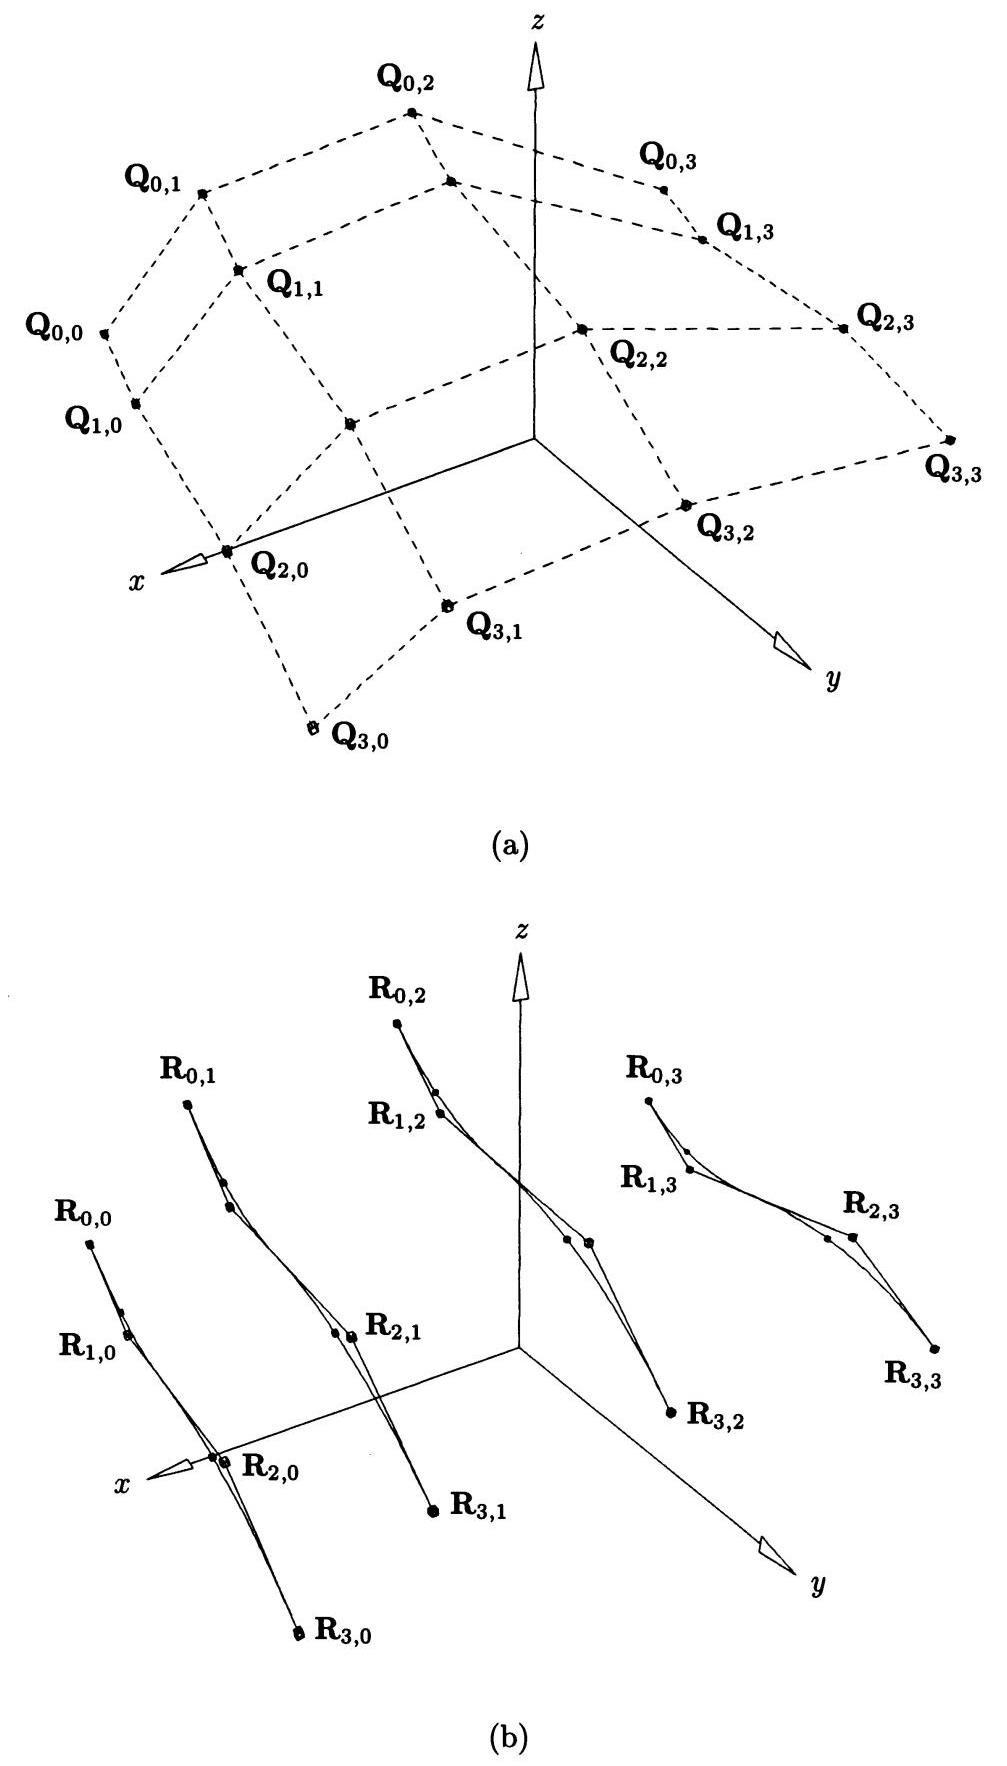
\includegraphics[max width=0.9\textwidth]{images/0193ba0d-ab19-7138-9798-cb281ce60de0_386_264_246_1007_1766_0.jpg}
\end{center}
\hspace*{3em} 

图 9.14. 全局表面插值。 (a) 数据点；(b) 插值 \(u\) -方向数据点；(c) 通过控制点在 \(v\) 方向进行插值。

\begin{center}
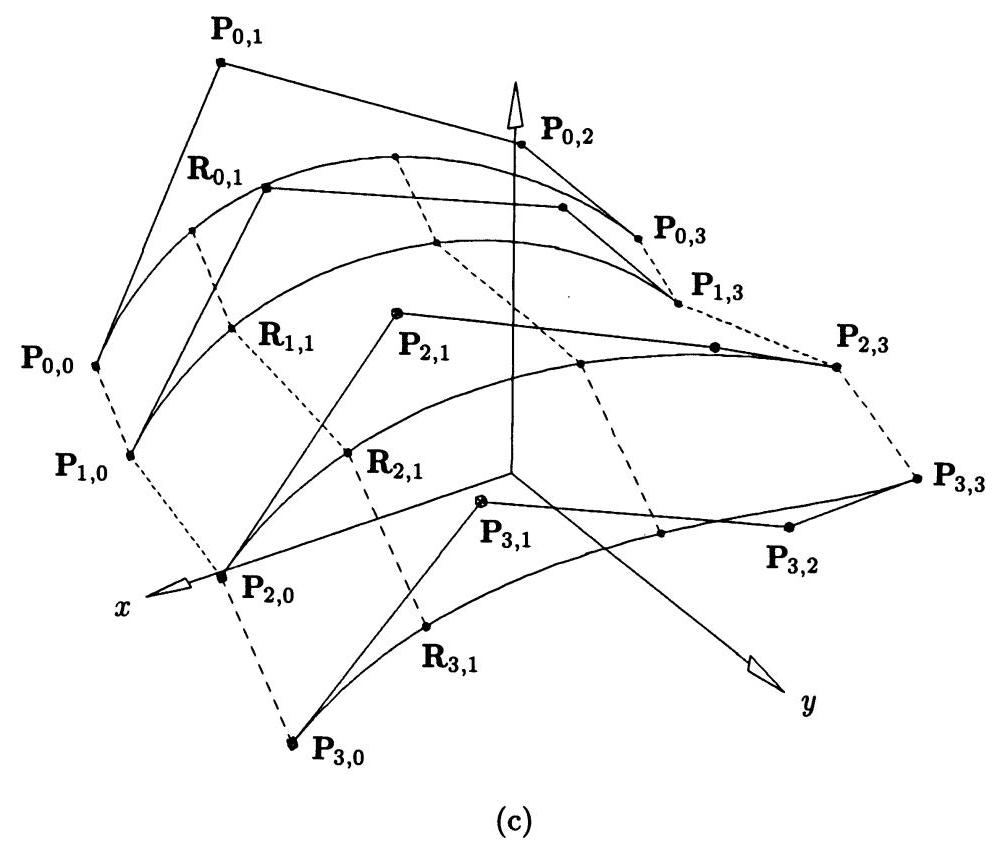
\includegraphics[max width=0.9\textwidth]{images/0193ba0d-ab19-7138-9798-cb281ce60de0_387_262_264_1000_844_0.jpg}
\end{center}
\hspace*{3em} 

图 9.14. (续)。

总结来说，表面插值的过程如下:

\HRule

ALGORITHM A9.4

\hspace*{2em} GlobalSurfInterp(n, m, Q, p, q, U, V, P)

\hspace*{5em} \{ /* Global surface interpolation */

\hspace*{8em} /* Input: n, m, Q, p, q */

\hspace*{8em} /* Output: U, V, P */

\hspace*{5em} SurfMeshParams \(\left( {n,m,Q,{uk},{vl}}\right) ;\;/ *\) get parameters \(*\) /

\hspace*{5em} Compute U using Eq. (9.8);

\hspace*{5em} Compute V using Eq. (9.8);

\hspace*{5em} for (l=0; l<=m; l++)

\hspace*{7em} \{

\hspace*{7em} Do curve interpolation through \(Q\left\lbrack  0\right\rbrack  \left\lbrack  1\right\rbrack  ,\ldots ,Q\left\lbrack  n\right\rbrack  \left\lbrack  1\right\rbrack\) ;

\hspace*{7em} This yields \(R\left\lbrack  0\right\rbrack  \left\lbrack  1\right\rbrack  ,\ldots ,R\left\lbrack  n\right\rbrack  \left\lbrack  1\right\rbrack\) ;

\hspace*{7em} \}

\hspace*{5em} for (i = 0; i<=n; i++)

\hspace*{7em} \{

\hspace*{7em} Do curve interpolation through \(R\left\lbrack  i\right\rbrack  \left\lbrack  0\right\rbrack  ,\ldots ,R\left\lbrack  i\right\rbrack  \left\lbrack  m\right\rbrack\) ;

\hspace*{7em} This yields \(P\left\lbrack  i\right\rbrack  \left\lbrack  0\right\rbrack  ,\ldots ,P\left\lbrack  i\right\rbrack  \left\lbrack  m\right\rbrack\) ;

\hspace*{7em} \}

\hspace*{4em} \}

\HRule

图 9.15-9.18 显示了几个表面插值的例子。数据集在图 9.15 中展示。图 \({9.16}\mathrm{a} - {9.16}\mathrm{c}\) 中展示了具有不同参数化和节点向量的表面。度数为 (2,3)，参数化和节点向量是均匀的(图 9.16a)；弦长，通过平均获得的节点(图 9.16b)；以及向心，通过平均获得的节点(图 9.16c)。在图 9.17 中描绘了具有不同度数的表面插值。每个图的度数为:图 9.17a，度数 (2,3)；图 9.17b，度数 (3,2)；以及图 \({9.17}\mathrm{c}\) ，度数 (3,3)。在图 9.18 中演示了无法处理共面的数据。

\begin{center}
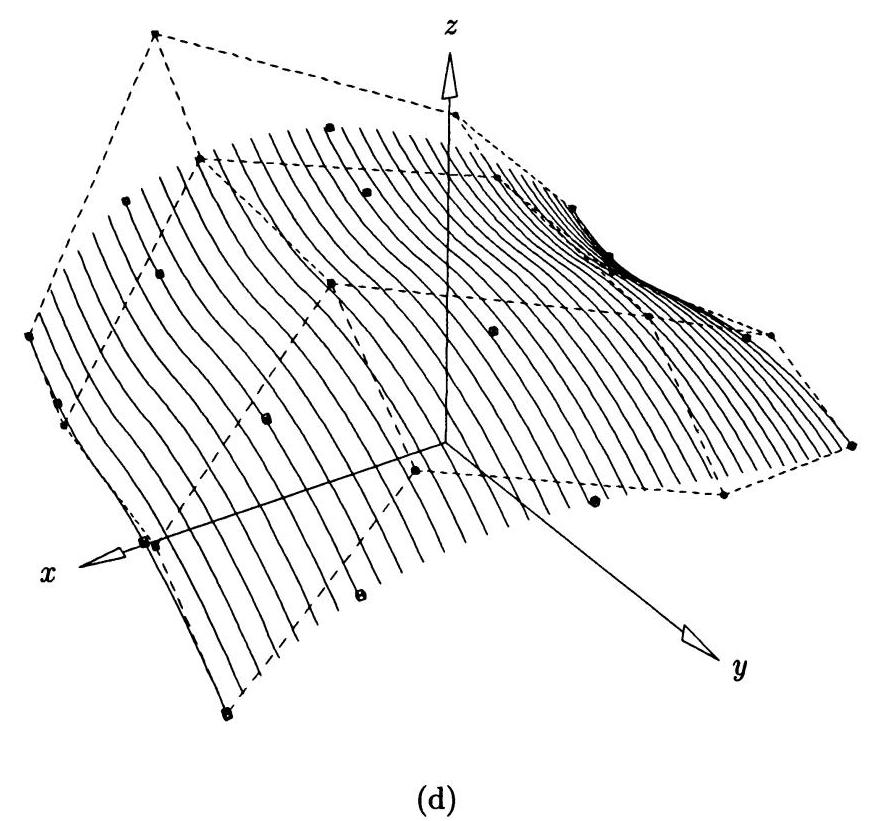
\includegraphics[max width=0.8\textwidth]{images/0193ba0d-ab19-7138-9798-cb281ce60de0_388_339_244_876_821_0.jpg}
\end{center}
\hspace*{3em} 

图 9.14. (续)。

\begin{center}
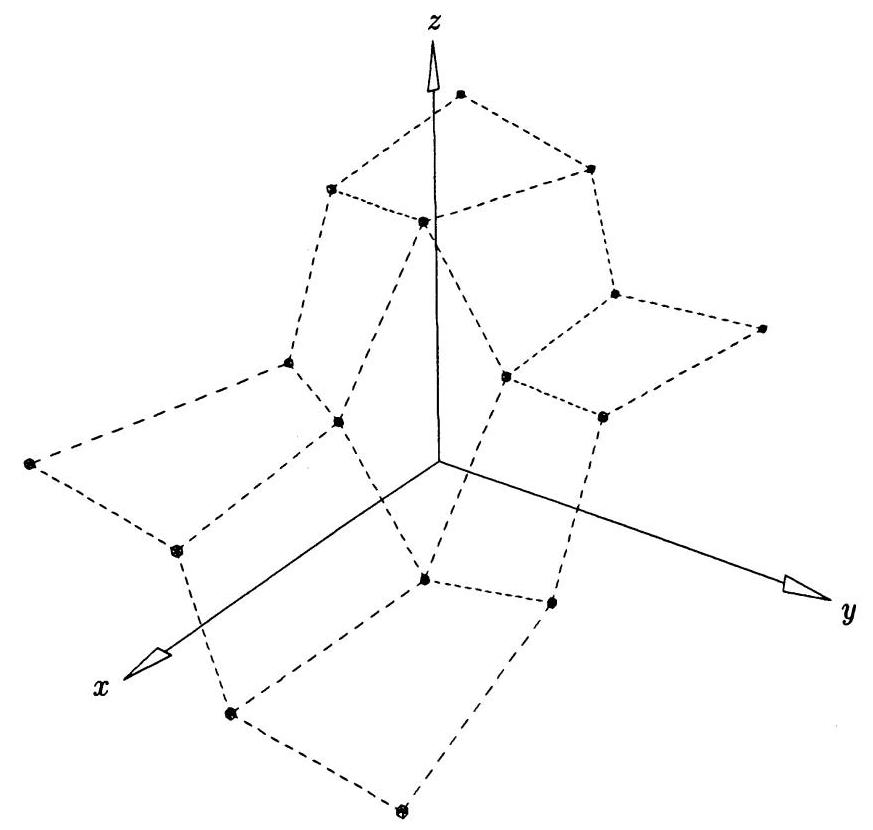
\includegraphics[max width=0.8\textwidth]{images/0193ba0d-ab19-7138-9798-cb281ce60de0_388_330_1235_873_830_0.jpg}
\end{center}
\hspace*{3em} 

图 9.15. 用于测试表面插值的数据点。

导数约束也可以纳入全局表面插值。从概念上讲，第2章和第3章的导数公式可以用来为每个指定的导数约束定义一个额外的线性方程。不幸的是，如果每一行或每一列的数据约束数量不相同，使用两方向的曲线插值来求解未知的表面控制点将变得更加困难，如前所述。然而，通过巧妙地使用曲线节点插入和表面节点移除，可以调整算法A9.4以处理个别数据点的偏导数约束。最后，局部表面插值方法(见第9.3节)非常适合处理导数约束，因为它们在每个点上都需要导数。



\section{局部插值}

在本节中，我们介绍曲线和表面对点和切线数据的局部插值。我们从一些初步概念开始。

\subsection{局部曲线插值初步}

设定 \(\left\{  {\mathbf{Q}}_{k}\right\}  ,k = 0,\ldots ,n\) 。局部曲线插值是指构造 \(n\) 多项式或有理曲线段 \({\mathbf{C}}_{i}\left( u\right) ,i =\)  \(0,\ldots ,n - 1\) 的一种方法，使得 \({\mathbf{Q}}_{i}\) 和 \({\mathbf{Q}}_{i + 1}\) 是 \({\mathbf{C}}_{i}\left( u\right)\) 的端点。相邻的段以某种规定的连续性水平连接，构造过程通常从左到右逐段进行。任何产生的方程仅与少数相邻段局部相关。在NURBS框架下，我们使用多项式或有理Bézier曲线构造这些段，然后通过选择合适的节点向量获得NURBS曲线。

现在让 \({\bar{u}}_{i}\) 表示 \({\mathbf{C}}_{i}\left( u\right)\) 的起始参数和 \({\mathbf{C}}_{i - 1}\left( u\right)\) 的结束参数。如果它们的切线方向在 \({\bar{u}}_{i}\) 处重合，即 \({\mathbf{C}}_{i}^{\prime }\left( {\bar{u}}_{i}\right)\) 和 \({\mathbf{C}}_{i - 1}^{\prime }\left( {\bar{u}}_{i}\right)\) 指向相同方向，则 \({\mathbf{C}}_{i}\left( u\right)\) 和 \({\mathbf{C}}_{i - 1}\left( u\right)\) 在 \({\bar{u}}_{i}\) 处具有 \({G}^{1}\) 连续性(对于几何而言为 \(G\) )。然而，它们的大小可能不同。 \({G}^{1}\) 连续性意味着曲线在视觉上是连续的(光滑的)，但在参数化上可能存在不连续性。关于 \({G}^{n}\) 连续性的更深入研究，读者可以参考 Barsky 和 DeRose [Bars89,90]。局部拟合算法旨在提供某种程度的 \(G\) 或 \(C\) 连续性；在本章中，我们仅介绍提供 \({G}^{1}\) 或 \({C}^{1}\) 连续性的算法。产生更高连续性的局部方法并不广泛使用。尽管 \({G}^{2}\) 和 \({C}^{2}\) 在三次曲线中是可能的，但如果要保持合理的灵活性，则必须使用更高的次数。

\begin{center}
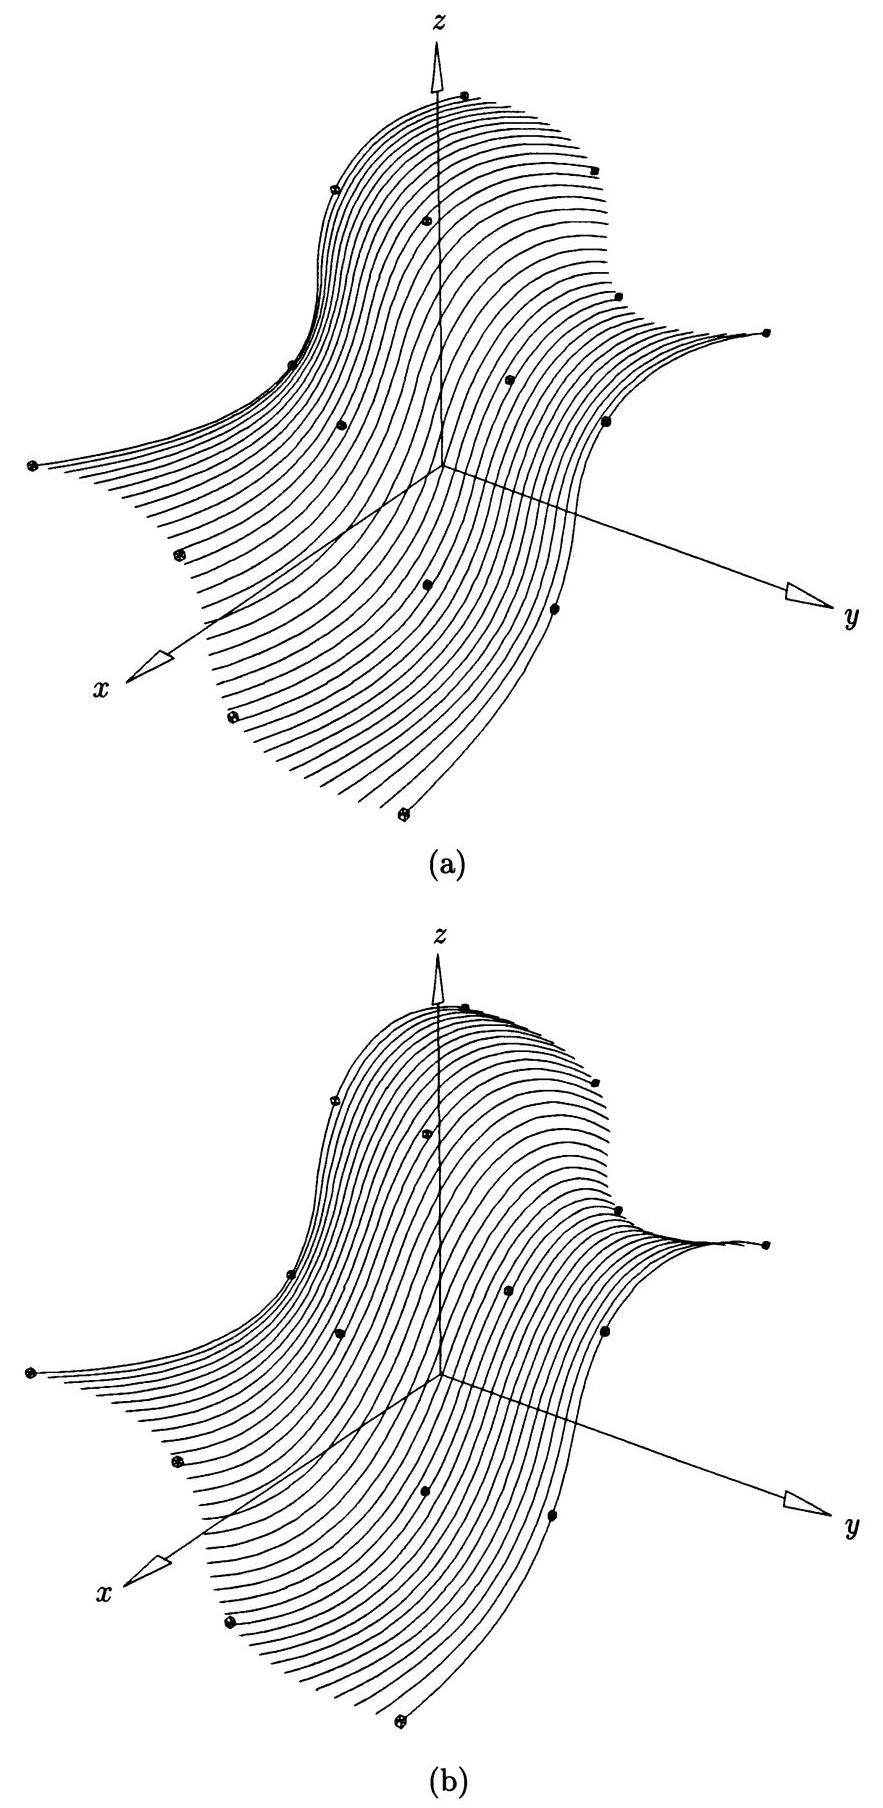
\includegraphics[max width=0.8\textwidth]{images/0193ba0d-ab19-7138-9798-cb281ce60de0_390_327_243_883_1808_0.jpg}
\end{center}
\hspace*{3em} 

图 9.16. 通过使用不同的参数化和节点向量获得的度数为(2,3)的曲面插值。

\begin{center}
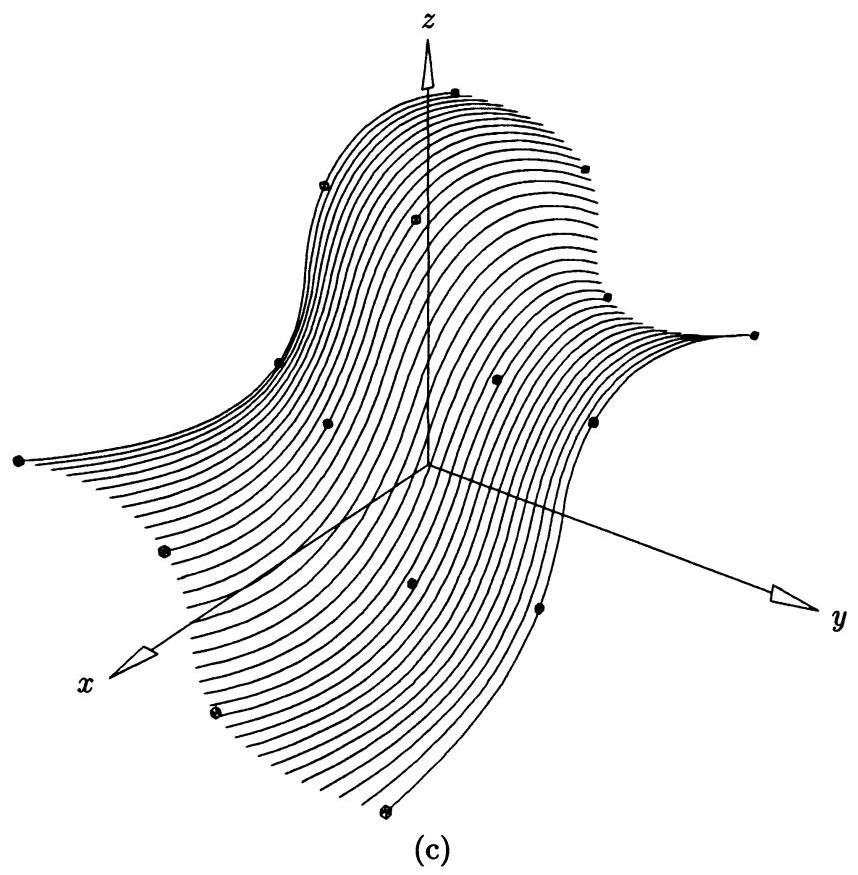
\includegraphics[max width=0.7\textwidth]{images/0193ba0d-ab19-7138-9798-cb281ce60de0_391_344_255_858_875_0.jpg}
\end{center}
\hspace*{3em} 

图 9.16.(续。)

获取 Bézier 段 \({\mathbf{C}}_{i}\left( u\right)\) 需要计算内部 Bézier 控制点，对于二次曲线需要一个点，对于三次曲线需要两个点。这些控制点位于与曲线在 \({\mathbf{Q}}_{k}\) 处相切的直线上；因此，我们需要在每个 \({\mathbf{Q}}_{k}\) 处的切向量 \({\mathbf{T}}_{k}\) 。在某些情况下，它们可以与 \({\mathbf{Q}}_{k}\) 一起输入；例如，当计算两个表面之间的交点时，它们很容易获得。然而，如果没有输入，则必须作为拟合算法的一部分进行计算。有多种方法可供选择；Boehm 等人 [Boeh84] 对各种方法进行了综述。让

\[
\Delta {\bar{u}}_{k} = {\bar{u}}_{k} - {\bar{u}}_{k - 1}\;{\mathbf{q}}_{k} = {\mathbf{Q}}_{k} - {\mathbf{Q}}_{k - 1}\;{\mathbf{d}}_{k} = \frac{{\mathbf{q}}_{k}}{\Delta {\bar{u}}_{k}}
\]

所有方法有两种形式之一

\[
{\mathbf{D}}_{k} = \left( {1 - {\alpha }_{k}}\right) {\mathbf{d}}_{k} + {\alpha }_{k}{\mathbf{d}}_{k + 1} \tag{9.28}
\]

或

\[
{\mathbf{T}}_{k} = \frac{{\mathbf{V}}_{k}}{\left| {\mathbf{V}}_{k}\right| }\;{\mathbf{V}}_{k} = \left( {1 - {\alpha }_{k}}\right) {\mathbf{q}}_{k} + {\alpha }_{k}{\mathbf{q}}_{k + 1} \tag{9.29}
\]

(见图 9.19)。注意，方程 (9.28) 假设 \({\bar{u}}_{k}\) 的值已经被指定。向量 \({\mathbf{D}}_{k}\) 可以被视为导数的估计值。

\begin{center}
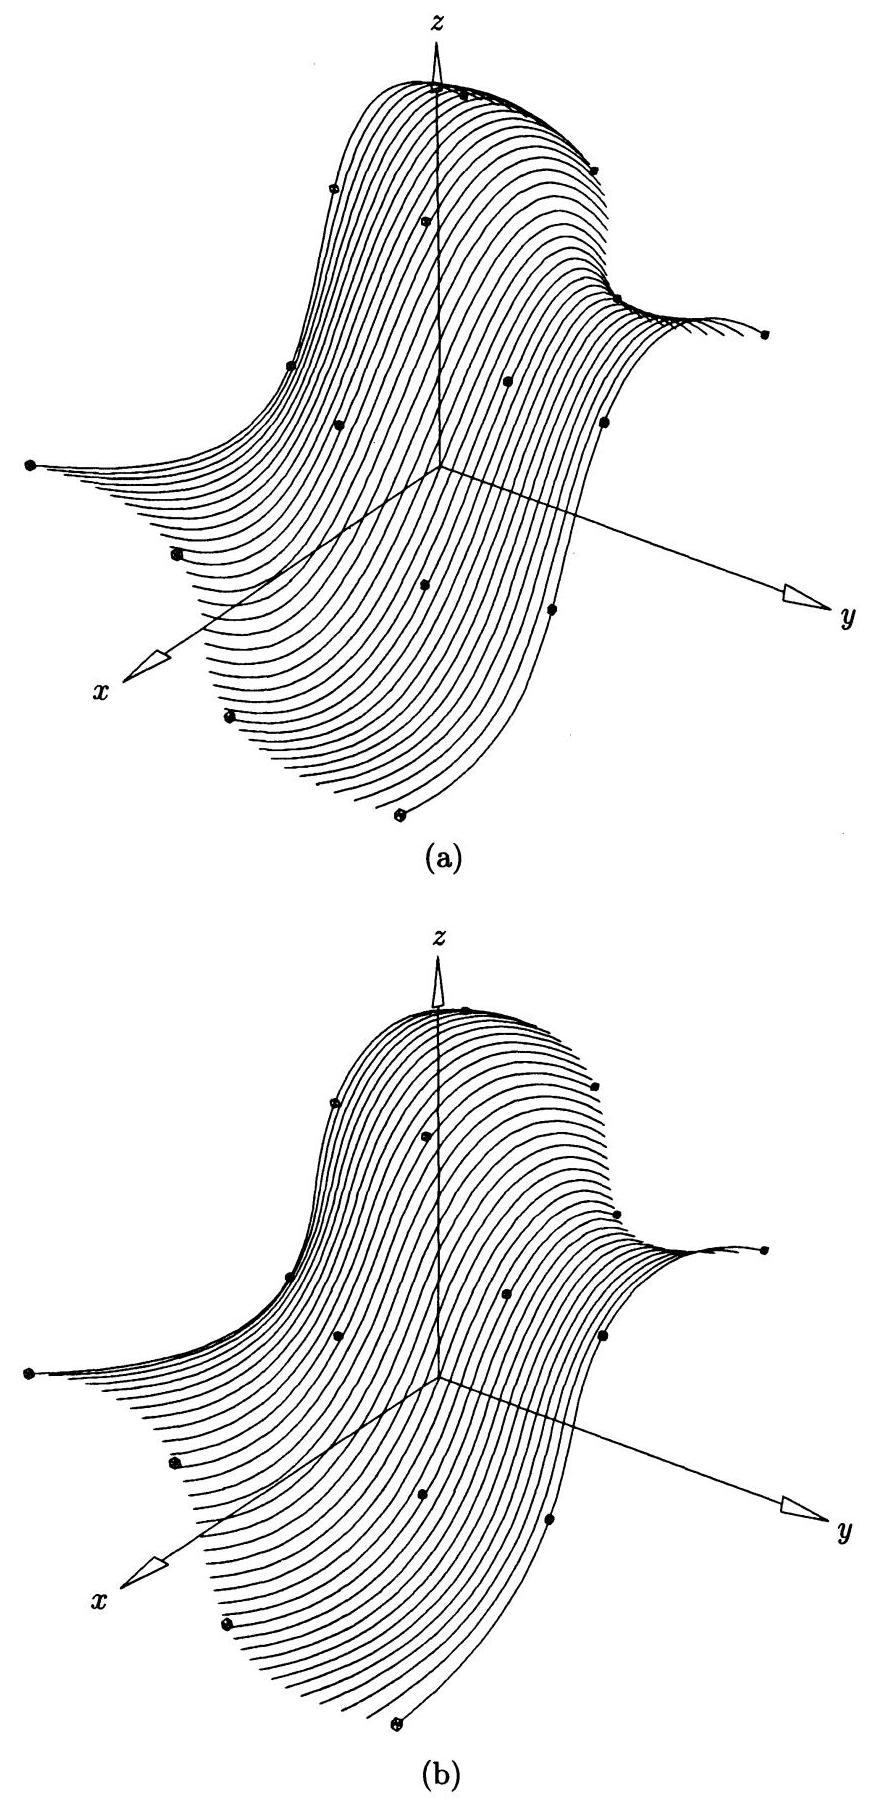
\includegraphics[max width=0.8\textwidth]{images/0193ba0d-ab19-7138-9798-cb281ce60de0_392_332_242_881_1802_0.jpg}
\end{center}
\hspace*{3em} 

图 9.17. 使用不同次数的表面插值；参数化是弦长，节点向量通过平均获得。

\begin{center}
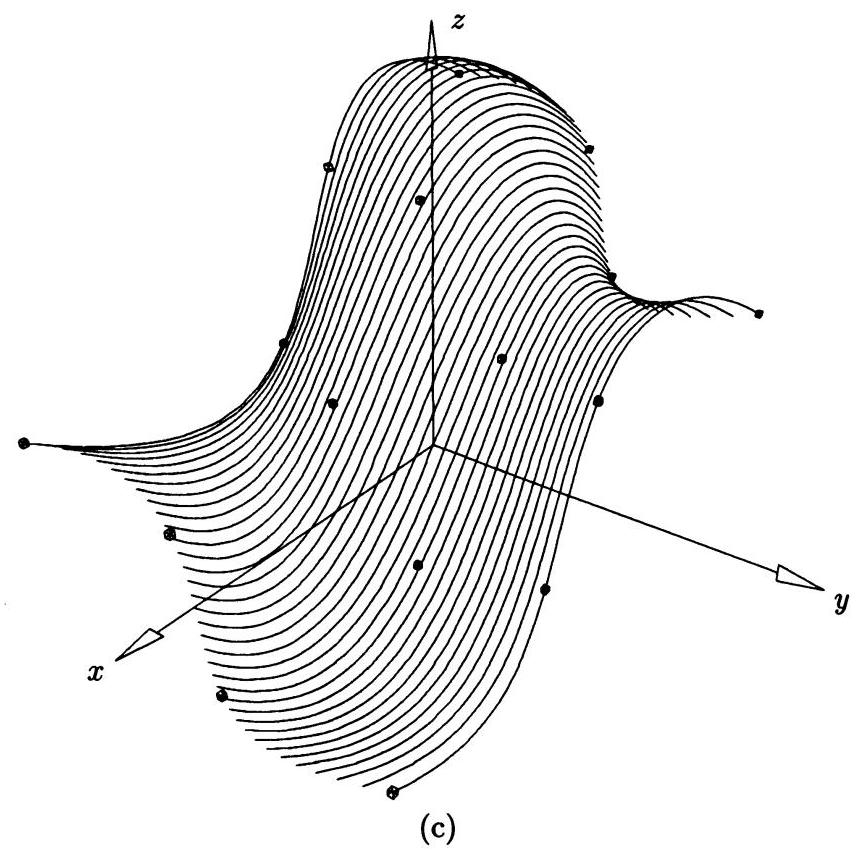
\includegraphics[max width=0.7\textwidth]{images/0193ba0d-ab19-7138-9798-cb281ce60de0_393_340_255_861_852_0.jpg}
\end{center}
\hspace*{3em} 

图 9.17. (续)

方程 (9.29) 不使用参数 \({\bar{u}}_{k}\) ，因此得到的向量应仅视为切向方向。幅度和参数的分配必须相互结合进行；它们不是独立的。还要注意，我们严格使用符号 \(\mathbf{T}\) 来表示单位长度的切向量。方程 (9.28) 和 (9.29) 是线性插值。各种方案在计算插值参数 \({\alpha }_{k}\) 的方式上有所不同；它通常依赖于三个或五个邻近点。例如，贝塞尔方法 [DeBo78] 是一种三点法，使用

\[
{\alpha }_{k} = \frac{\Delta {\bar{u}}_{k}}{\Delta {\bar{u}}_{k} + \Delta {\bar{u}}_{k + 1}}\;k = 1,\ldots ,n - 1 \tag{9.30}
\]

结合方程 (9.28)。设定

\[
{\alpha }_{k} = \frac{\left| {\mathbf{q}}_{k - 1} \times  {\mathbf{q}}_{k}\right| }{\left| {{\mathbf{q}}_{k - 1} \times  {\mathbf{q}}_{k}}\right|  + \left| {{\mathbf{q}}_{k + 1} \times  {\mathbf{q}}_{k + 2}}\right| }\;k = 2,\ldots ,n - 2 \tag{9.31}
\]

与方程 (9.29) 一起得出一种五点法来获得 \({\mathbf{T}}_{k}\) [Akim70; Renn82; Pieg87d]。它的优点在于三个共线点 \({\mathbf{Q}}_{k - 1},{\mathbf{Q}}_{k}\) 、 \({\mathbf{Q}}_{k + 1}\) 产生一个与线段平行的 \({\mathbf{T}}_{k}\) 。如果 \({\mathbf{Q}}_{k - 2},{\mathbf{Q}}_{k - 1},{\mathbf{Q}}_{k}\) 共线且 \({\mathbf{Q}}_{k},{\mathbf{Q}}_{k + 1},{\mathbf{Q}}_{k + 2}\) 共线，则方程 (9.31) 的分母消失。这意味着在 \({\mathbf{Q}}_{k}\) 处要么是一个拐角，要么是从 \({\mathbf{Q}}_{k - 2}\) 到 \({\mathbf{Q}}_{k + 2}\) 的一条直线段。在这些情况下， \({\alpha }_{k}\) 可以通过多种方式定义；我们选择

\begin{center}
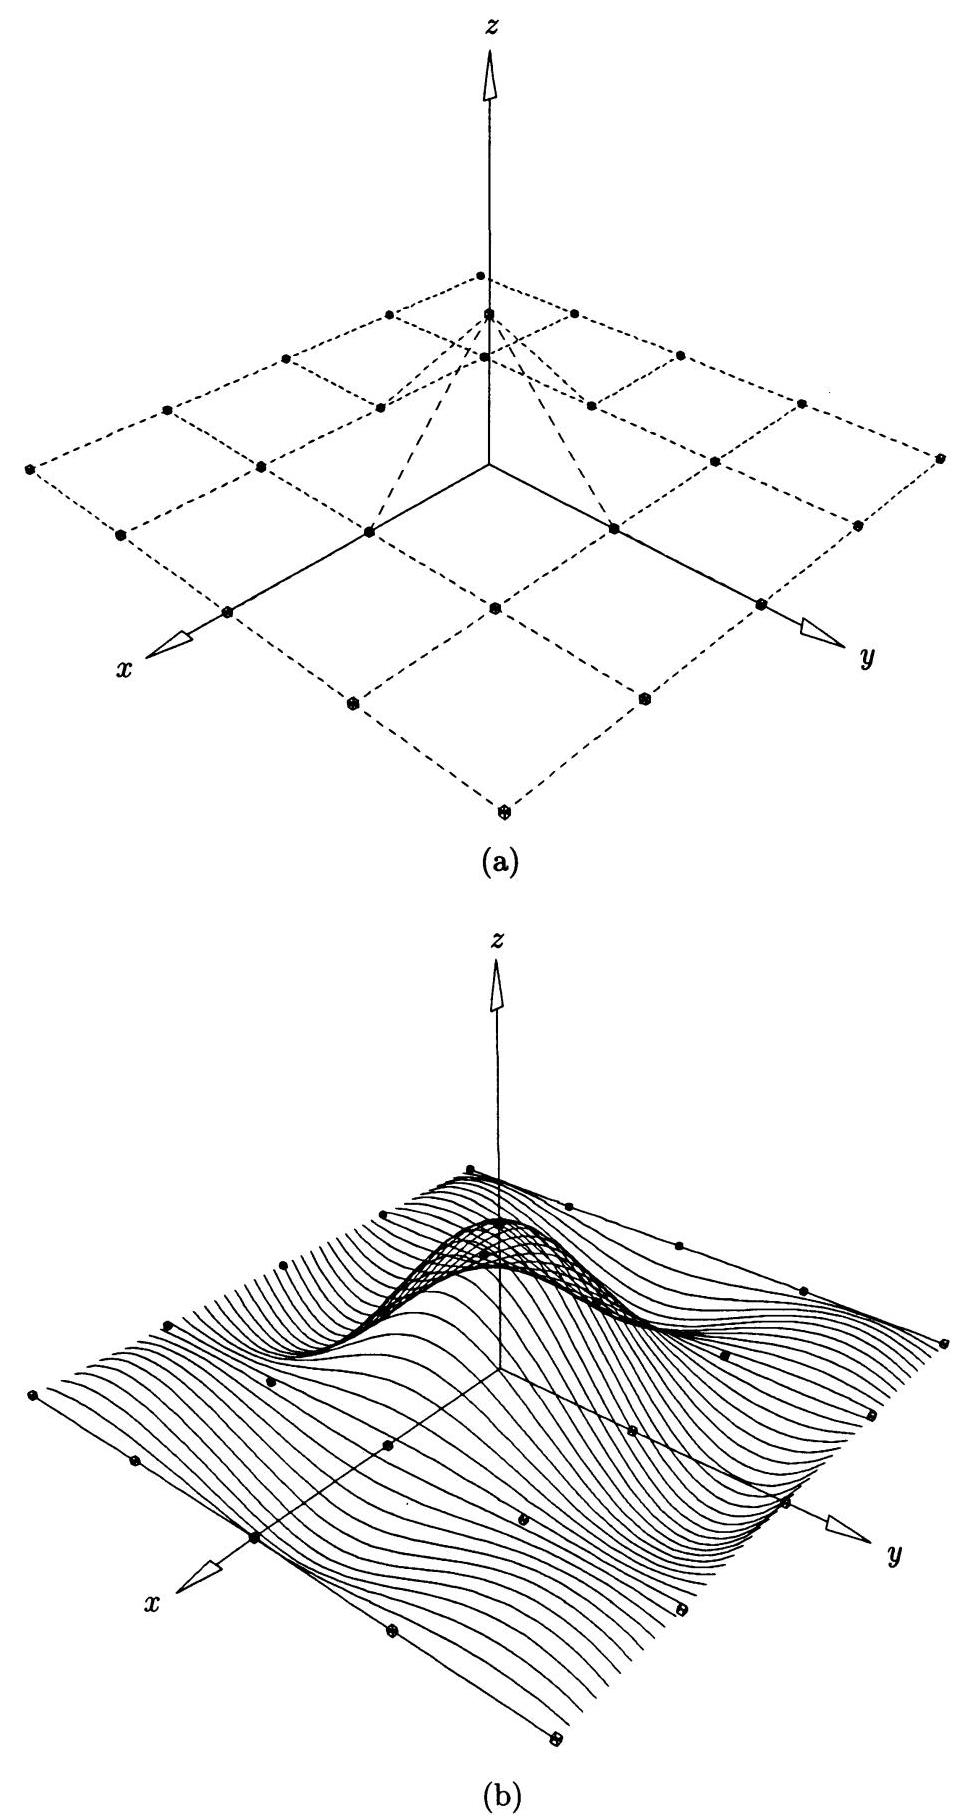
\includegraphics[max width=0.8\textwidth]{images/0193ba0d-ab19-7138-9798-cb281ce60de0_394_273_246_975_1816_0.jpg}
\end{center}
\hspace*{3em} 

图 9.18. 全局表面插值示例。(a) 包含共面的数据点；(b) 插值表面。

\begin{center}
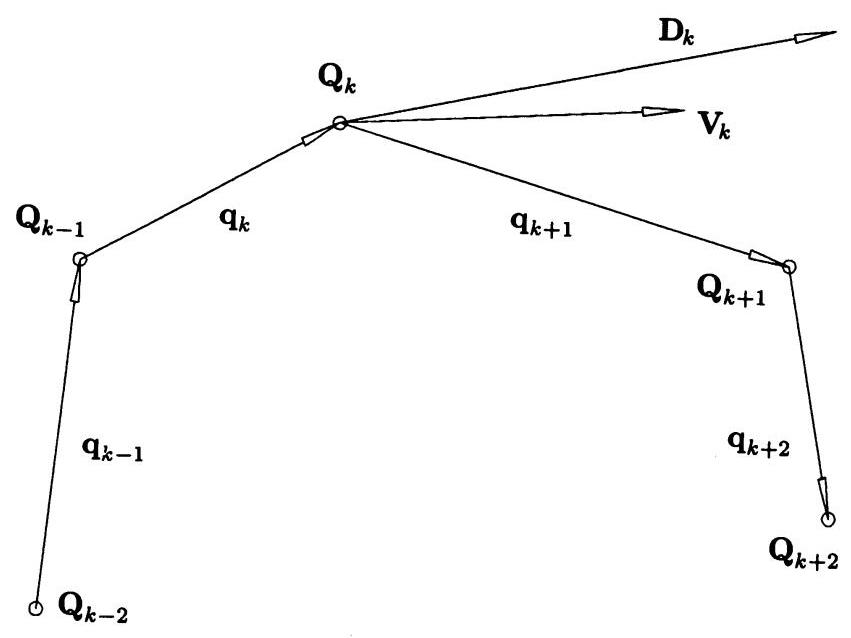
\includegraphics[max width=0.7\textwidth]{images/0193ba0d-ab19-7138-9798-cb281ce60de0_395_344_270_851_638_0.jpg}
\end{center}
\hspace*{3em} 

图 9.19. 局部曲线插值的切线 \(\left( {\mathbf{V}}_{k}\right)\) 和导数 \(\left( {\mathbf{D}}_{k}\right)\) 向量的计算。

\begin{itemize}
\item \({\alpha }_{k} = 1\) ，这意味着 \({\mathbf{V}}_{k} = {\mathbf{q}}_{k + 1}\) ；如果数据暗示，则在 \({\mathbf{Q}}_{k}\) 处产生一个拐角；
\end{itemize}

\begin{itemize}
\item \({\alpha }_{k} = 1/2\) ，这意味着 \({\mathbf{V}}_{k} = 1/2\left( {{\mathbf{q}}_{k} + {\mathbf{q}}_{k + 1}}\right)\) ；这个选择在暗示有拐角的情况下使拐角平滑。
\end{itemize}

基于这些选择，局部曲线插值例程可以接受一个输入标志，指示是否保留拐角。所有方法在端点处都需要特殊处理。对于三点方案，我们可以设置

\[
{\mathbf{D}}_{0} = 2{\mathbf{d}}_{1} - {\mathbf{D}}_{1}\;{\mathbf{D}}_{n} = 2{\mathbf{d}}_{n} - {\mathbf{D}}_{n - 1} \tag{9.32}
\]

对于五点方案，我们可以使用

\[
{\mathbf{q}}_{0} = 2{\mathbf{q}}_{1} - {\mathbf{q}}_{2}\;{\mathbf{q}}_{-1} = 2{\mathbf{q}}_{0} - {\mathbf{q}}_{1}
\]

\[
{\mathbf{q}}_{n + 1} = 2{\mathbf{q}}_{n} - {\mathbf{q}}_{n - 1}\;{\mathbf{q}}_{n + 2} = 2{\mathbf{q}}_{n + 1} - {\mathbf{q}}_{n} \tag{9.33}
\]

以替代方程 (9.31) 和 (9.29)，以获得 \({\mathbf{T}}_{0},{\mathbf{T}}_{1}\) 和 \({\mathbf{T}}_{n - 1},{\mathbf{T}}_{n}\) 。我们现在准备介绍几种局部插值方法。



\subsection{局部抛物线曲线插值}

我们从一个简单的二维非理性二次方案开始。设 \(\left\{  {\mathbf{Q}}_{k}\right\}  ,k = 0,\ldots ,n\) 为 \({xy}\) 平面中的点。使用某种切线估计方案来计算相应的 \(\left\{  {\mathbf{T}}_{k}\right\}\) ，例如，方程 (9.29)、(9.31) 和 (9.33)。设 \({L}_{k}\) 表示由 \(\left( {{\mathbf{Q}}_{k},{\mathbf{T}}_{k}}\right)\) 定义的有向线， \({\mathbf{R}}_{k}\) 为 \({L}_{k - 1}\) 和 \({L}_{k}\) 的交点。暂时假设交点存在，

并且

\[
{\gamma }_{k - 1} > 0\;{\gamma }_{k} < 0 \tag{9.34}
\]

其中

\[
{\mathbf{R}}_{k} = {\mathbf{Q}}_{k - 1} + {\gamma }_{k - 1}{\mathbf{T}}_{k - 1}\;{\mathbf{R}}_{k} = {\mathbf{Q}}_{k} + {\gamma }_{k}{\mathbf{T}}_{k}
\]

(我们稍后会去掉这个限制)。然后我们选择作为控制点

\[
{\mathbf{Q}}_{0},{\mathbf{R}}_{1},{\mathbf{Q}}_{1},{\mathbf{R}}_{2},\ldots ,{\mathbf{R}}_{n},{\mathbf{Q}}_{n} \tag{9.35}
\]

设 \({\bar{u}}_{0} = 0\) 和 \({\bar{u}}_{n} = 1\) 。如果 \(\left\{  {\bar{u}}_{i}\right\}  ,i = 1,\ldots ,n - 1\) 是满足 \({\bar{u}}_{i - 1} < {\bar{u}}_{i} < {\bar{u}}_{i + 1}\) 的任意数列，则方程 (9.35) 的控制点以及节点向量

\[
U = \left\{  {0,0,0,{\bar{u}}_{1},{\bar{u}}_{1},{\bar{u}}_{2},{\bar{u}}_{2},\ldots ,{\bar{u}}_{n - 1},{\bar{u}}_{n - 1},1,1,1}\right\}   \tag{9.36}
\]

定义了一个非理性、 \({G}^{1}\) 连续的二次 B 样条曲线，插值 \(\left\{  {\mathbf{Q}}_{k}\right\}\) (见图 9.20)。内部节点的选择不会影响曲线的形状，仅影响参数化。可以选择节点，使得得到的曲线是 \({C}^{1}\) 连续的；在这样做时，我们可以去掉控制点 \({\mathbf{Q}}_{1},\ldots ,{\mathbf{Q}}_{n - 1}\) 和每个内部节点的一个出现。我们简单地在 \({\mathbf{Q}}_{k - 1}\) 处使起始和结束导数相等(使用方程 [3.7] 转换到区间 \(\left\lbrack  {{\bar{u}}_{k - 2},{\bar{u}}_{k - 1}}\right\rbrack\) 和 \(\left. \left\lbrack  {{\bar{u}}_{k - 1},{\bar{u}}_{k}}\right\rbrack  \right)\) )，并得到公式

\[
{\bar{u}}_{0} = 0\;{\bar{u}}_{1} = 1
\]

\[
{\bar{u}}_{k} = {\bar{u}}_{k - 1} + \left( {{\bar{u}}_{k - 1} - {\bar{u}}_{k - 2}}\right) \frac{\left| {\mathbf{R}}_{k} - {\mathbf{Q}}_{k - 1}\right| }{\left| {\mathbf{Q}}_{k - 1} - {\mathbf{R}}_{k - 1}\right| }\;k = 2,\ldots ,n \tag{9.37}
\]

插值 \(\left\{  {\mathbf{Q}}_{k}\right\}\) 的 \({C}^{1}\) 连续曲线由控制点定义

\[
{\mathbf{Q}}_{0},{\mathbf{R}}_{1},{\mathbf{R}}_{2},\ldots ,{\mathbf{R}}_{n - 1},{\mathbf{R}}_{n},{\mathbf{Q}}_{n} \tag{9.38}
\]

\begin{center}
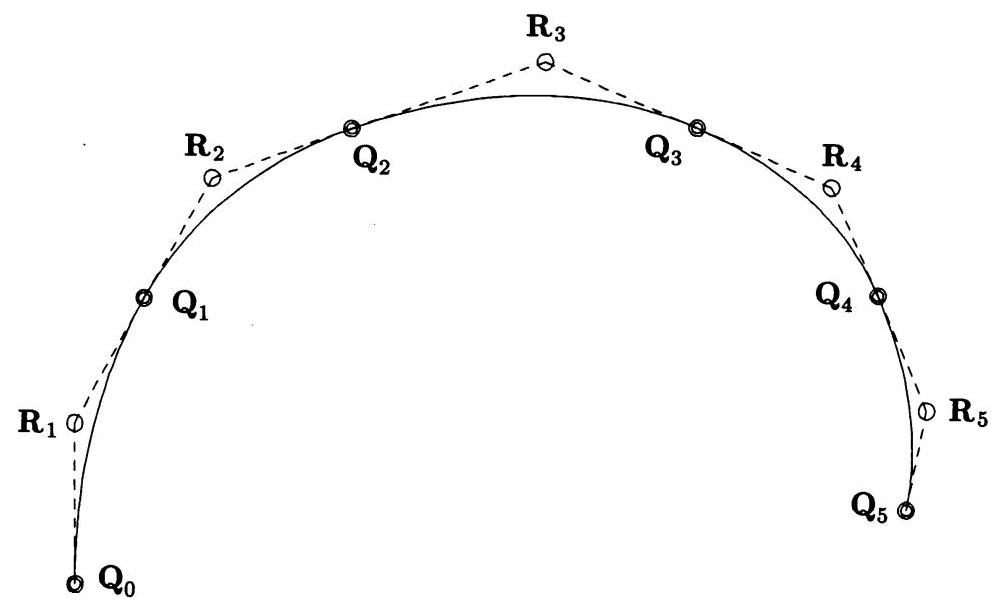
\includegraphics[max width=0.9\textwidth]{images/0193ba0d-ab19-7138-9798-cb281ce60de0_396_263_1474_1001_611_0.jpg}
\end{center}
\hspace*{3em} 

图 9.20. \({G}^{1}\) 连续二次曲线插值。

和节点

\[
U = \left\{  {0,0,0,\frac{{\bar{u}}_{1}}{{\bar{u}}_{n}},\frac{{\bar{u}}_{2}}{{\bar{u}}_{n}},\ldots ,\frac{{\bar{u}}_{n - 2}}{{\bar{u}}_{n}},\frac{{\bar{u}}_{n - 1}}{{\bar{u}}_{n}},1,1,1}\right\}   \tag{9.39}
\]

为了实现 \({C}^{1}\) 的连续性和控制点数量的减少，必须付出代价，即在参数化方面；图 9.21a 和 9.21b 显示了这一点。这些图中的曲线在等间距的参数值处标记。在图 9.21a 中，节点是使用公式 (9.37) 计算的，而在图 9.21b 中则使用了弦长参数化 (公式 [9.5])。请注意 \({\mathbf{Q}}_{k}\) 的间距。

现在我们去掉公式 (9.34) 中给出的限制，并详细说明在计算 \({\mathbf{R}}_{k}\) 时出现的两个特殊情况:

\begin{itemize}
\item \({\mathbf{T}}_{k - 1}\) 和 \({\mathbf{T}}_{k}\) 是平行的，因此 \({\mathbf{R}}_{k}\) 不能通过交点计算；这可能表示共线段、拐点或曲线中的 \({180}^{ \circ  }\) 转弯；
\end{itemize}

\begin{itemize}
\item \({\mathbf{R}}_{k}\) 可以计算，但 \({\gamma }_{k - 1}\) 和 \({\gamma }_{k}\) 不满足公式 (9.34)；这表明要么是拐点，要么是超过 \({180}^{ \circ  }\) 的转弯。
\end{itemize}

如果 \({\mathbf{T}}_{k - 1}\) 和 \({\mathbf{T}}_{k}\) 都平行于弦 \({\mathbf{Q}}_{\mathbf{k} - \mathbf{1}}{\mathbf{Q}}_{\mathbf{k}}\) ，则适用共线段情况。我们通过设置简单地处理此情况

\begin{center}
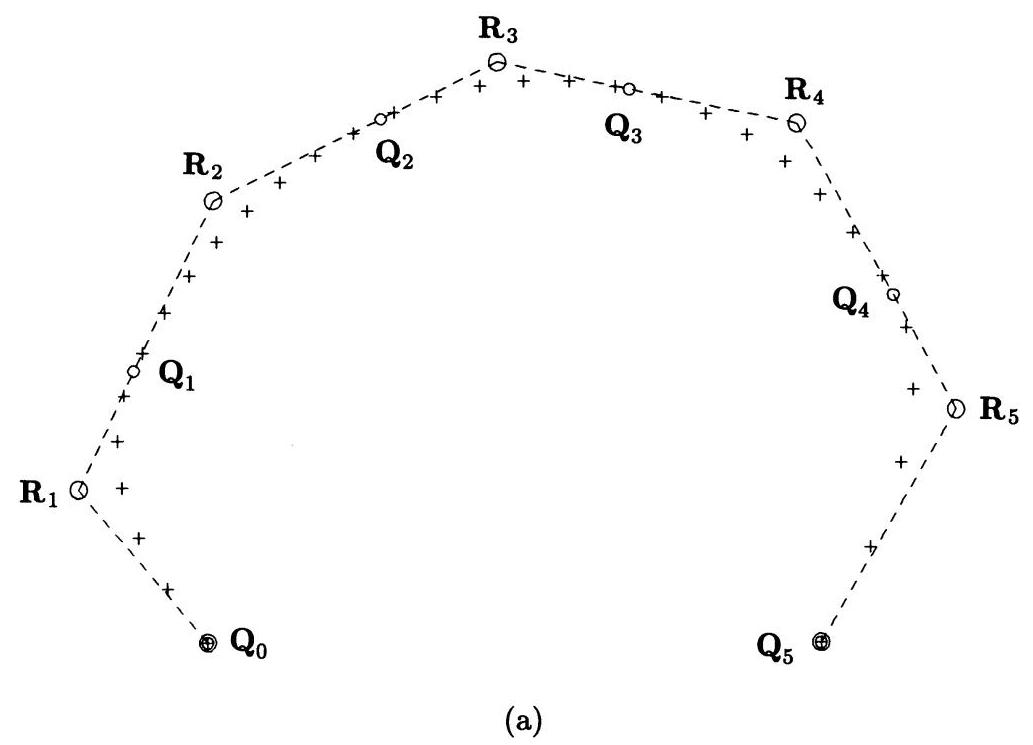
\includegraphics[max width=0.9\textwidth]{images/0193ba0d-ab19-7138-9798-cb281ce60de0_397_252_1317_1033_745_0.jpg}
\end{center}
\hspace*{3em} 

图 9.21. 图 9.20 中曲线插值的参数化。(a) \({C}^{1}\) 参数化 (公式 [9.39]-[9.41])；(b) 使用弦长参数的 \({G}^{1}\) 参数化。

\begin{center}
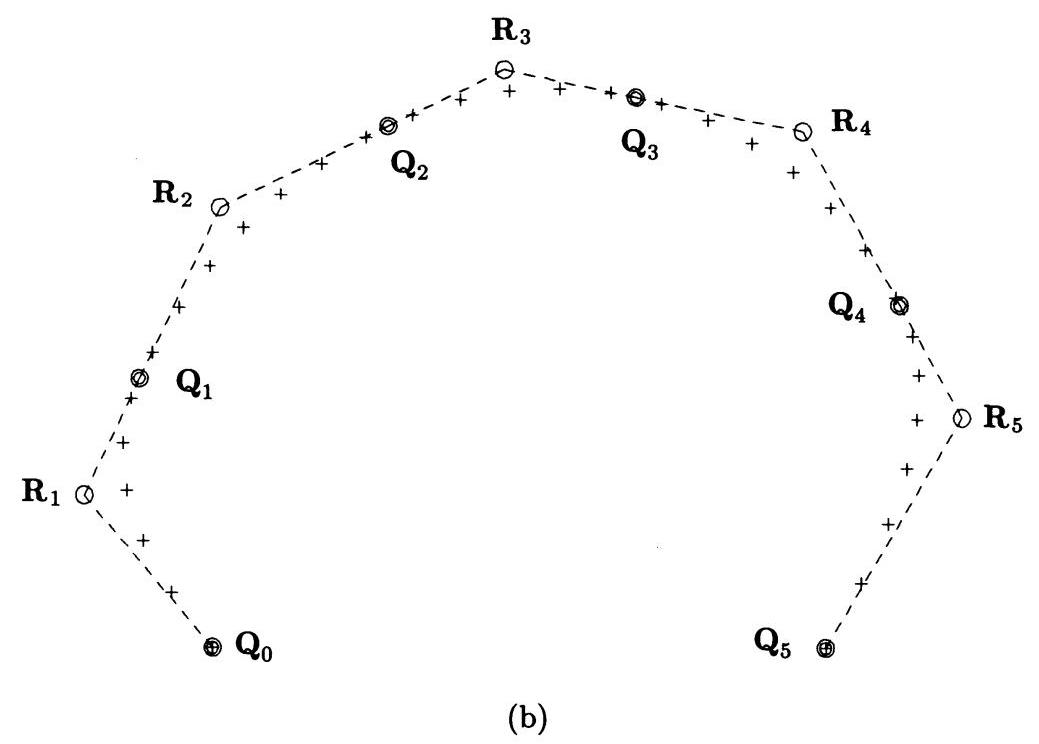
\includegraphics[max width=0.9\textwidth]{images/0193ba0d-ab19-7138-9798-cb281ce60de0_398_248_250_1039_744_0.jpg}
\end{center}
\hspace*{3em} 

图 9.21. (续)

\[
{\mathbf{R}}_{k} = \frac{1}{2}\left( {{\mathbf{Q}}_{k - 1} + {\mathbf{Q}}_{k}}\right)  \tag{9.40}
\]

所有其他特殊情况通过在 \({\mathbf{Q}}_{\mathbf{k} - \mathbf{1}}\) 和 \({\mathbf{Q}}_{k}\) 之间创建两个抛物线段而不是一个来处理。因此，我们必须计算三个额外的点， \({\mathbf{R}}_{k}^{\prime },{\mathbf{Q}}_{k}^{\prime }\) 和 \({\mathbf{R}}_{k + 1}^{\prime }\) (见图 9.22a 和 9.22b)。设置

\[
{\mathbf{R}}_{k}^{\prime } = {\mathbf{Q}}_{k - 1} + {\gamma }_{k}{\mathbf{T}}_{k - 1}\;{\mathbf{R}}_{k + 1}^{\prime } = {\mathbf{Q}}_{k} - {\gamma }_{k + 1}{\mathbf{T}}_{k} \tag{9.41}
\]

和

\[
{\mathbf{Q}}_{k}^{\prime } = \frac{{\gamma }_{k}{\mathbf{R}}_{k + 1}^{\prime } + {\gamma }_{k + 1}{\mathbf{R}}_{k}^{\prime }}{{\gamma }_{k} + {\gamma }_{k + 1}} \tag{9.42}
\]

仍需确定 \({\gamma }_{k}\) 和 \({\gamma }_{k + 1}\) 的合理选择。如果 \({\mathbf{T}}_{k - 1}\) 和 \({\mathbf{T}}_{k}\) 是平行的(但不与 \({\mathbf{Q}}_{k - 1}{\mathbf{Q}}_{k}\) 平行)，则设置

\[
{\gamma }_{k} = {\gamma }_{k + 1} = \frac{1}{2}\left| {{\mathbf{Q}}_{k - 1}{\mathbf{Q}}_{k}}\right|  \tag{9.43}
\]

这一点在图 9.22a 中得到了说明，针对 \({180}^{ \circ  }\) 转弯的情况。现在考虑 \({\mathbf{T}}_{k - 1}\) 和 \({\mathbf{T}}_{k}\) 不平行的情况，但方程 (9.34) 不成立(见图 9.22b)。直观上， \({\gamma }_{k}\) 和 \({\gamma }_{k + 1}\) 应该依赖于弦 \({\mathbf{Q}}_{k - 1}{\mathbf{Q}}_{k}\) 和切线 \({\mathbf{T}}_{k - 1}\) 和 \({\mathbf{T}}_{k}\) 所夹的角度 \({\theta }_{k - 1}\) 和 \({\theta }_{k}\) ，分别 \(\left( {0 \leq  {\theta }_{k - 1},{\theta }_{k} \leq  {90}^{ \circ  }}\right)\) 。图 \({9.22}\mathrm{c}\) 显示了由等腰三角形定义的抛物线。对于这个图，可以很容易推导出

\[
{\gamma }_{k} = {\gamma }_{k + 1} = \frac{1}{4}\frac{\left| {\mathbf{Q}}_{k - 1}{\mathbf{Q}}_{k}\right| }{\cos \theta }
\]

这暗示着设置

\[
{\gamma }_{k} = \frac{1}{4}\frac{\left| {\mathbf{Q}}_{k - 1}{\mathbf{Q}}_{k}\right| }{\alpha \cos {\theta }_{k} + \left( {1 - \alpha }\right) \cos {\theta }_{k - 1}}
\]

\begin{center}
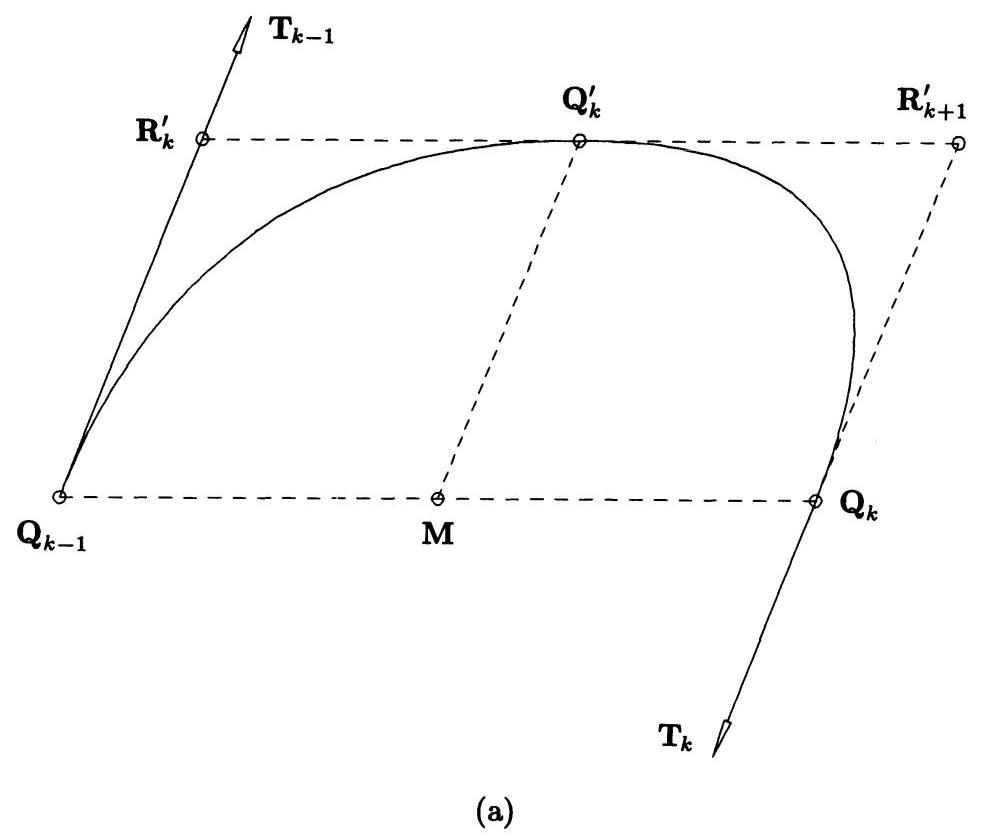
\includegraphics[max width=0.9\textwidth]{images/0193ba0d-ab19-7138-9798-cb281ce60de0_399_280_253_984_836_0.jpg}
\end{center}
\hspace*{3em} 

图 9.22. 计算在邻近数据点处切线的分段抛物线弧。(a) 平行的端切线；(b) 切线 \({\mathbf{T}}_{k - 1}\) 和 \({\mathbf{T}}_{k}\) 所暗示的转折点；(c) 由等腰控制三角形定义的抛物线。

\[
{\gamma }_{k + 1} = \frac{1}{4}\frac{\left| {\mathbf{Q}}_{k - 1}{\mathbf{Q}}_{k}\right| }{\alpha \cos {\theta }_{k - 1} + \left( {1 - \alpha }\right) \cos {\theta }_{k}} \tag{9.44}
\]

其中 \(\alpha\) 是介于 0 和 1 之间的某个常数。基于实验观察，我们选择 \(\alpha  = 2/3\) 。图 \({9.22}\mathrm{\;b}\) 的两个曲线段是使用方程 (9.41)、(9.42) 和 (9.44) 得到的。

图 9.23-9.25 显示了几个示例。在图 9.23a 中，切线是通过贝塞尔方法 [DeBo78] 计算的，而在图 9.23b 中使用了 Akima 方法 [Akim70]。注意图 9.23b 中如何保持共线性。在图 9.24a 中选择了“无拐角”选项，导致每个段之间产生了(可能不希望的)平滑连接。图 9.24b 显示了保持拐角的情况，使用相同的算法，仅更改了标志设置。图 9.25 显示了使用该插值方法获得的鞋底轮廓。


\subsection{局部有理二次曲线插值}

前述方法可以修改为生成有理二次曲线。所有在 \({\mathbf{Q}}_{k}\) 的权重设置为 1；在 \({\mathbf{R}}_{k}\) 的权重可以自由选择。例如，一些应用可能希望段更“圆形”而不是抛物线形。更具体地，对于 \(k = 1,\ldots ,n\) ，定义了一个圆锥弧

\begin{center}
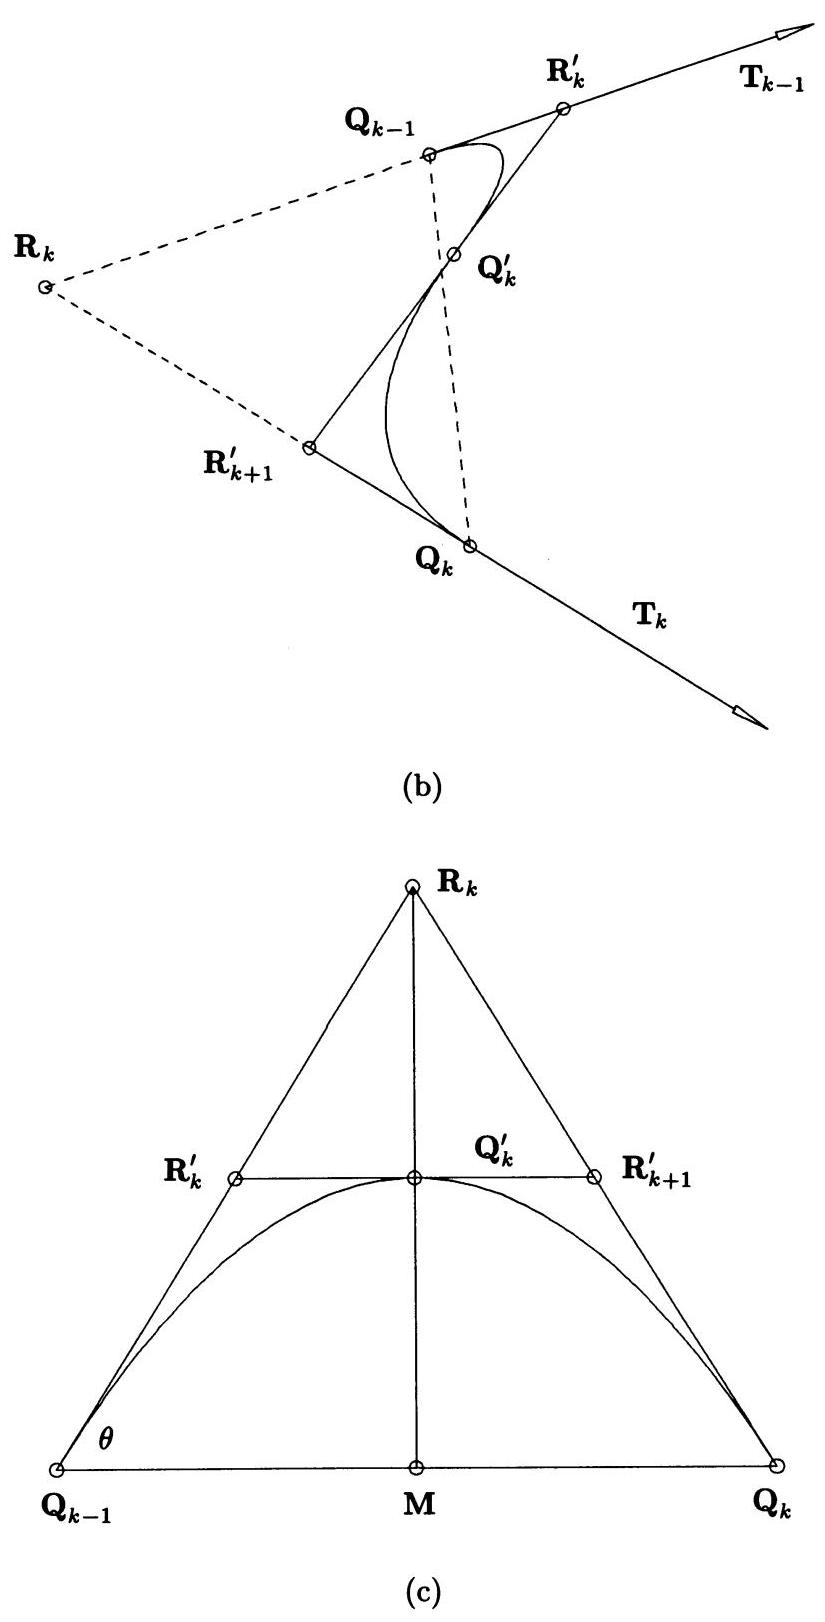
\includegraphics[max width=0.7\textwidth]{images/0193ba0d-ab19-7138-9798-cb281ce60de0_400_353_236_825_1622_0.jpg}
\end{center}
\hspace*{3em} 

图 9.22. (续。)

由 \({\mathbf{Q}}_{k - 1},{\mathbf{R}}_{k},{\mathbf{Q}}_{k}\) 定义，权重 \({w}_{k}\) 在 \({\mathbf{R}}_{k}\) 处。可以按如下方式设置 \({w}_{k}\) :

1. 如果 \({\mathbf{Q}}_{k - 1},{\mathbf{R}}_{k}\) 和 \({\mathbf{Q}}_{k}\) 共线，则设置 \({w}_{k} = 1\) ；

2. 如果三角形是等腰三角形 \(\left( {\left| {{\mathbf{Q}}_{k - 1}{\mathbf{R}}_{k}}\right|  = \left| {{\mathbf{Q}}_{k}{\mathbf{R}}_{k}}\right| }\right)\) ，则根据方程 (7.33) 设置 \({w}_{k}\) (一个精确的圆弧)；

\begin{center}
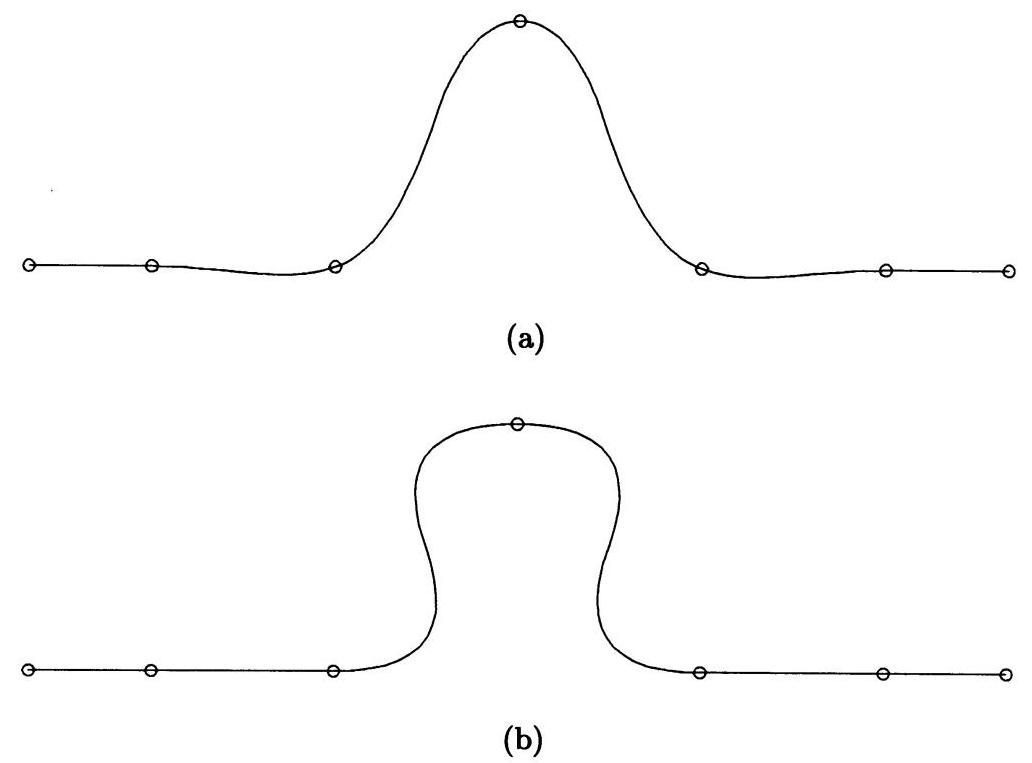
\includegraphics[max width=0.9\textwidth]{images/0193ba0d-ab19-7138-9798-cb281ce60de0_401_254_254_1032_763_0.jpg}
\end{center}
\hspace*{3em} 

图 9.23. 局部二次曲线插值。 (a) 通过贝塞尔方法计算的切线；(b) 通过 Akima 方法计算的切线。

3. 如果三角形不是等腰的，则按如下方式设置 \({w}_{k}\) (见图 9.26):

a. 让 \(\mathbf{M} = 1/2\left( {{\mathbf{Q}}_{k - 1} + {\mathbf{Q}}_{k}}\right)\) ;

b. 设定 \({\mathbf{S}}_{1}\) 为 \({\mathbf{{MR}}}_{k}\) 的交点，与角的平分线 \(\angle {\mathbf{R}}_{k}{\mathbf{Q}}_{k - 1}{\mathbf{Q}}_{k}\) 。

c. 设定 \({\mathbf{S}}_{2}\) 为 \({\mathbf{{MR}}}_{k}\) 的交点，与角的平分线 \(\angle {\mathbf{Q}}_{k - 1}{\mathbf{Q}}_{k}{\mathbf{R}}_{k}\) 。

d. 设定 \(\mathbf{S} = 1/2\left( {{\mathbf{S}}_{1} + {\mathbf{S}}_{2}}\right)\) ;

e. 以 \(\mathbf{S}\) 作为肩点，使用方程 (7.30) 和 (7.31) 计算 \({w}_{k}\) 。

在计算 \({\mathbf{R}}_{k}\) 的特殊情况下的识别正如所详细描述的；然而，计算 \({\mathbf{R}}_{k}^{\prime }\) 和 \({\mathbf{R}}_{k + 1}^{\prime }\) 略有不同。再次参考图 \({9.22}\mathrm{c}\) ，但假设等腰三角形定义了一个圆弧，由方程 (7.31)-(7.33) 可得

\[
{\gamma }_{k} = \frac{1}{2}\frac{\left| {\mathbf{Q}}_{k - 1}{\mathbf{Q}}_{k}\right| }{1 + \cos \theta }
\]

因此，我们设定

\[
{\gamma }_{k} = \frac{1}{2}\frac{\left| {\mathbf{Q}}_{k - 1}{\mathbf{Q}}_{k}\right| }{1 + \alpha \cos {\theta }_{k} + \left( {1 - \alpha }\right) \cos {\theta }_{k - 1}}
\]

\[
{\gamma }_{k + 1} = \frac{1}{2}\frac{\left| {\mathbf{Q}}_{k - 1}{\mathbf{Q}}_{k}\right| }{1 + \alpha \cos {\theta }_{k - 1} + \left( {1 - \alpha }\right) \cos {\theta }_{k}} \tag{9.45}
\]

其中 \(\alpha\) 是与方程 (9.44) 中相同的常数。

\begin{center}
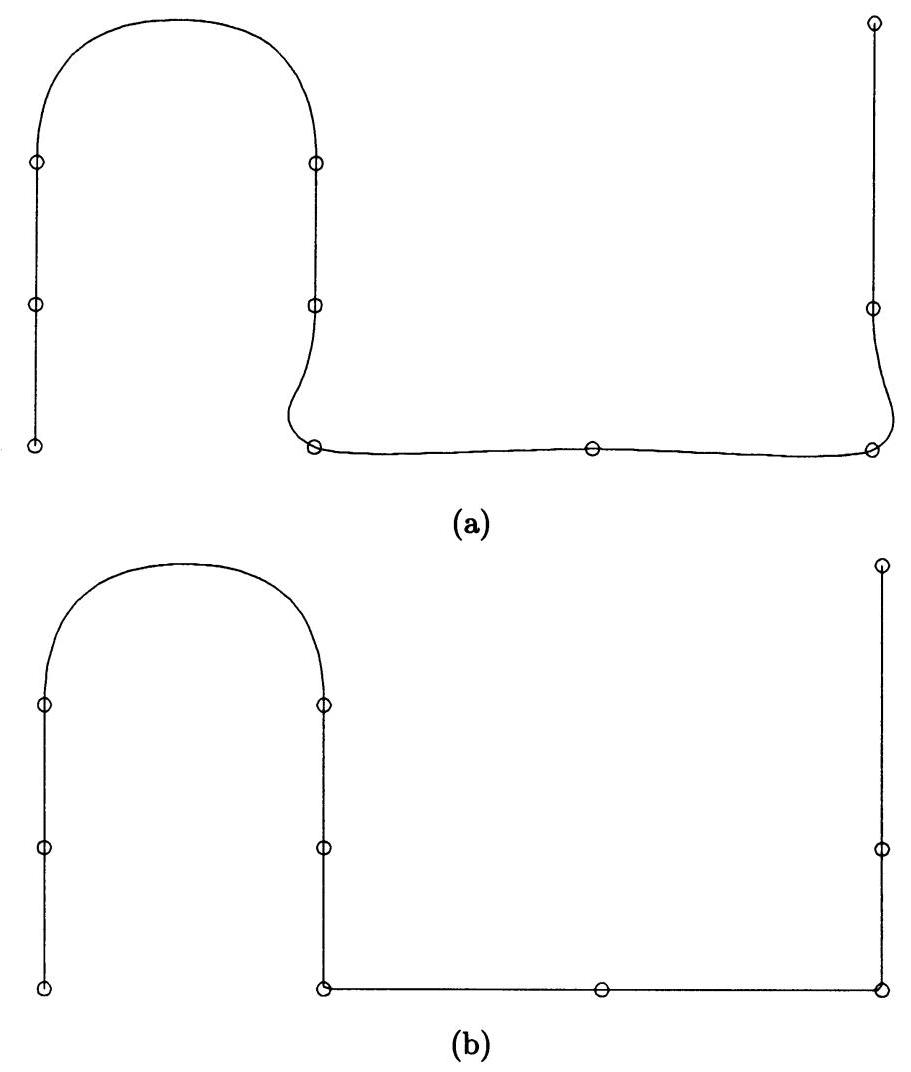
\includegraphics[max width=0.8\textwidth]{images/0193ba0d-ab19-7138-9798-cb281ce60de0_402_305_264_911_1072_0.jpg}
\end{center}
\hspace*{3em} 

图 9.24. 局部二次曲线插值。 (a) 不允许有角；(b) 保持角。

图 9.27 显示了有理二次曲线插值的一个例子。注意，从四个点精确重现了圆形，并且通过设置角标志保留了两个角。


\subsection{局部三次曲线插值}
三次曲线能够轻松处理三维数据和拐点，而无需特殊处理。我们首先推导出关于三次贝塞尔曲线的一般事实，这本身就是一个有趣的主题。设 \({\mathbf{P}}_{0}\) 和 \({\mathbf{P}}_{3}\) 为两个端点， \({\mathbf{T}}_{0}\) 和 \({\mathbf{T}}_{3}\) 为对应的单位长度切线方向。可以构造一条三次贝塞尔曲线 \(\mathbf{C}\left( u\right) ,u \in  \left\lbrack  {0,1}\right\rbrack\) ，其端点和切线方向满足

\[
\alpha  = \left| {{\mathbf{C}}^{\prime }\left( 0\right) }\right|  = \left| {{\mathbf{C}}^{\prime }\left( \frac{1}{2}\right) }\right|  = \left| {{\mathbf{C}}^{\prime }\left( 1\right) }\right|  \tag{9.46}
\]

\begin{center}
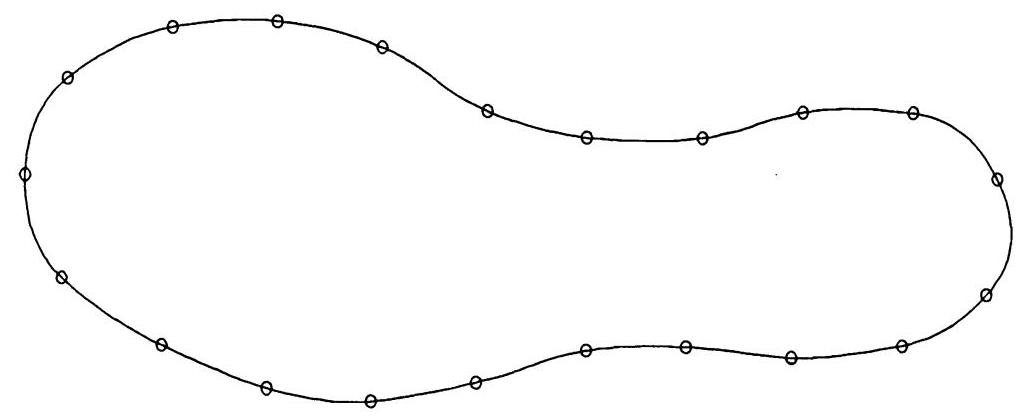
\includegraphics[max width=0.9\textwidth]{images/0193ba0d-ab19-7138-9798-cb281ce60de0_403_249_252_1026_420_0.jpg}
\end{center}
\hspace*{3em} 

图 9.25. 一段分段 \({G}^{1}\) 抛物线曲线插值。

(见图 9.28)，即速度在曲线的起点、中点和终点处是相等的。方程 (9.46) 和 (1.10) 暗示

\[
{\mathbf{P}}_{1} = {\mathbf{P}}_{0} + \frac{1}{3}\alpha {\mathbf{T}}_{0}\;{\mathbf{P}}_{2} = {\mathbf{P}}_{3} - \frac{1}{3}\alpha {\mathbf{T}}_{3} \tag{9.47}
\]

我们在 \(u = 1/2\) 处应用第一章的 deCasteljau 算法，并回忆该算法中使用的符号(见图 1.17)，我们写出 \({\mathbf{P}}_{0}^{3} = \mathbf{C}\left( {1/2}\right)\) 。通过反推 deCasteljau 算法，可以推导出

\[
{\mathbf{P}}_{1}^{2} - {\mathbf{P}}_{0}^{3} = \frac{1}{8}\left( {{\mathbf{P}}_{3} + {\mathbf{P}}_{2} - {\mathbf{P}}_{1} - {\mathbf{P}}_{0}}\right)  \tag{9.48}
\]

\begin{center}
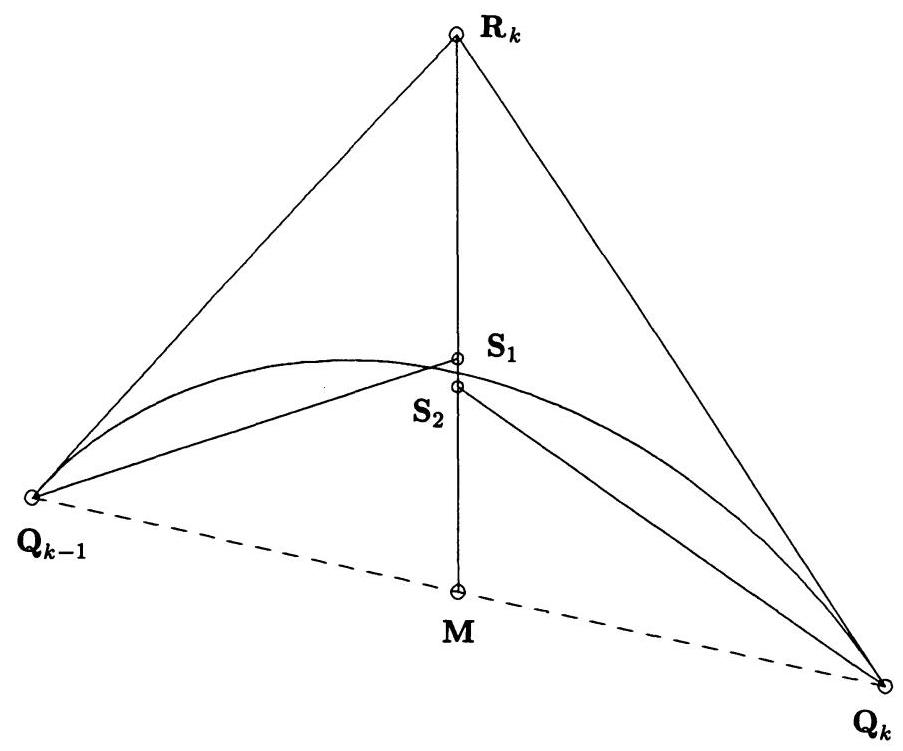
\includegraphics[max width=0.8\textwidth]{images/0193ba0d-ab19-7138-9798-cb281ce60de0_403_313_1318_903_751_0.jpg}
\end{center}
\hspace*{3em} 

图 9.26. 为有理二次插值选择权重(肩点)。

\begin{center}
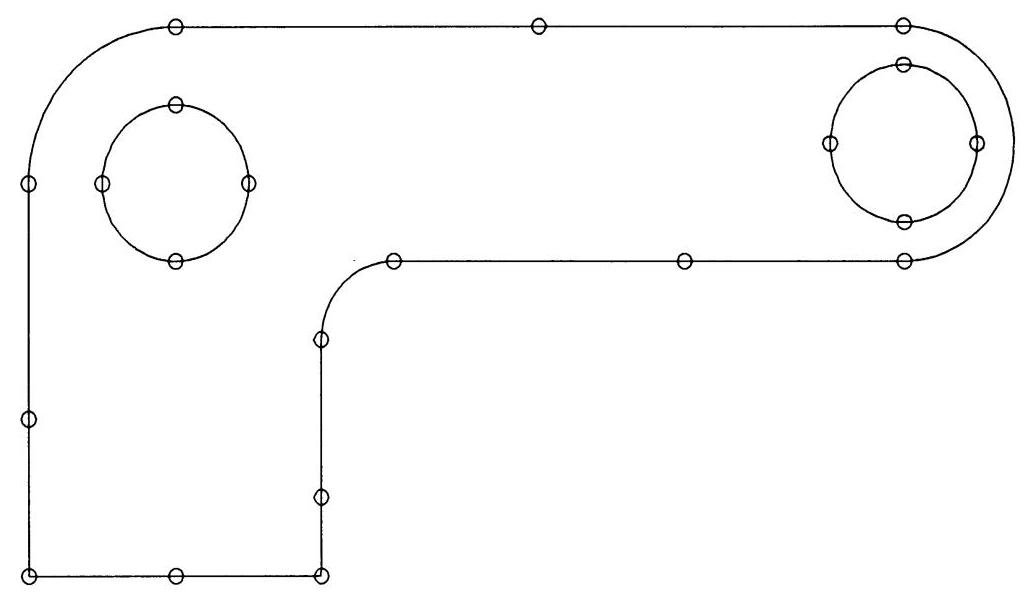
\includegraphics[max width=0.9\textwidth]{images/0193ba0d-ab19-7138-9798-cb281ce60de0_404_252_274_1033_597_0.jpg}
\end{center}
\hspace*{3em} 

图 9.27. 有理二次曲线插值；圆形被精确再现，角落保持不变。

应用方程 (1.10) 并考虑参数范围的二分法，它

得出

\[
{\mathbf{C}}^{\prime }\left( \frac{1}{2}\right)  = 6\left( {{\mathbf{P}}_{1}^{2} - {\mathbf{P}}_{0}^{3}}\right)  \tag{9.49}
\]

将速度设为 \(\alpha\) ，将方程 (9.48) 代入方程 (9.49)，并使用方程 (9.47)，我们得到

\[
\frac{8}{6}\alpha  = \left| {{\mathbf{P}}_{3} + {\mathbf{P}}_{2} - {\mathbf{P}}_{1} - {\mathbf{P}}_{0}}\right|
\]

\[
= \left| {{\mathbf{P}}_{3} + \left( {{\mathbf{P}}_{3} - \frac{1}{3}\alpha {\mathbf{T}}_{3}}\right)  - \left( {{\mathbf{P}}_{0} + \frac{1}{3}\alpha {\mathbf{T}}_{0}}\right)  - {\mathbf{P}}_{0}}\right|
\]

这导致

\[
{16}{\alpha }^{2} = {\alpha }^{2}{\left| {\mathbf{T}}_{0} + {\mathbf{T}}_{3}\right| }^{2} - {12\alpha }\left( {{\mathbf{P}}_{3} - {\mathbf{P}}_{0}}\right)  \cdot  \left( {{\mathbf{T}}_{0} + {\mathbf{T}}_{3}}\right)  + {36}{\left| {\mathbf{P}}_{3} - {\mathbf{P}}_{0}\right| }^{2}
\]

最终

\[
a{\alpha }^{2} + {b\alpha } + c = 0 \tag{9.50}
\]

在哪里

\[
a = {16} - {\left| {\mathbf{T}}_{0} + {\mathbf{T}}_{3}\right| }^{2}\;b = {12}\left( {{\mathbf{P}}_{3} - {\mathbf{P}}_{0}}\right)  \cdot  \left( {{\mathbf{T}}_{0} + {\mathbf{T}}_{3}}\right) \;c =  - {36}{\left| {\mathbf{P}}_{3} - {\mathbf{P}}_{0}\right| }^{2}
\]

方程 (9.50) 有两个实数解 \(\alpha\) ，一个是正数，一个是负数。将正数解代入方程 (9.47) 得到所需的 \({\mathbf{P}}_{1}\) 和 \({\mathbf{P}}_{2}\) 。

现在我们回到立方插值问题。设 \(\left\{  {\mathbf{Q}}_{k}\right\}  ,k = 0,\ldots ,n\) 为一组三维数据点。如果没有给出切向量，则计算它们(方程 [9.29]、[9.31] 和 [9.33])。我们必须构造一个立方 Bézier 曲线。

\begin{center}
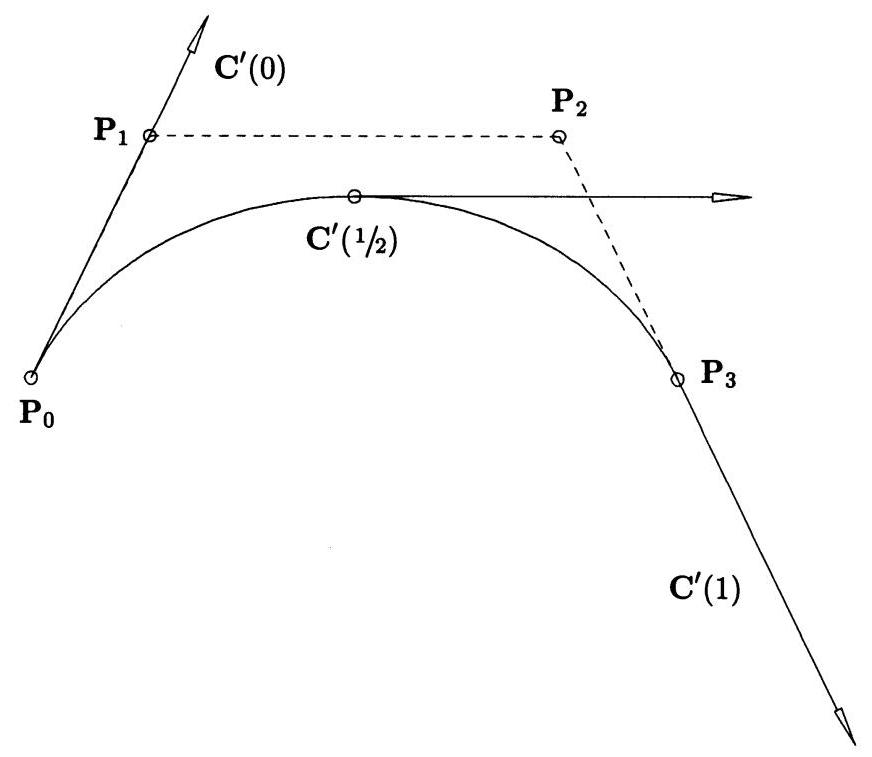
\includegraphics[max width=0.8\textwidth]{images/0193ba0d-ab19-7138-9798-cb281ce60de0_405_330_256_872_757_0.jpg}
\end{center}
\hspace*{3em} 

图 9.28。一个在参数 \(0,1/2\) 和 1 处具有相等切向量大小的立方 Bézier 曲线。

曲线段 \({\mathbf{C}}_{k}\left( u\right)\) 在每对 \({\mathbf{Q}}_{k},{\mathbf{Q}}_{k + 1}\) 之间。用 Bézier 控制点表示为

\[
{\mathbf{P}}_{k,0} = {\mathbf{Q}}_{k}\;{\mathbf{P}}_{k,1}\;{\mathbf{P}}_{k,2}\;{\mathbf{P}}_{k,3} = {\mathbf{Q}}_{k + 1} \tag{9.51}
\]

我们必须确定 \({\mathbf{P}}_{k,1}\) 和 \({\mathbf{P}}_{k,2}\) 在 \({\mathbf{T}}_{k}\) 和 \({\mathbf{T}}_{k + 1}\) 上的合适位置。可以获得一个 \({C}^{1}\) 连续立方体，并实现对均匀参数化的良好近似。该方法源于 Renner [Renn82]。真正的均匀参数化意味着在整个参数范围内的恒定速度。我们构造一条在每个 \({\mathbf{Q}}_{k}\) 及每个 Bézier 段的中点处速度相等的曲线。设定 \({\bar{u}}_{0} = 0\) 。现在，对于 \(k = 0,\ldots ,n - 1\) ， \({\bar{u}}_{k + 1}\) 和两个内控制点 \({\mathbf{C}}_{k}\left( u\right)\) 的计算如下:

1. 使用公式 (9.50) 计算 \(\alpha\) ，使用公式 (9.47) 计算 \({\mathbf{P}}_{k,1}\) 和 \({\mathbf{P}}_{k,2}\) ；

2. 设定

\[
{\bar{u}}_{k + 1} = {\bar{u}}_{k} + 3\left| {{\mathbf{P}}_{k,1} - {\mathbf{P}}_{k,0}}\right|  \tag{9.52}
\]

该算法产生 \(n\) Bézier 段，每个段在其参数范围的端点和中点处的速度均为 1， \(\left\lbrack  {{\bar{u}}_{k},{\bar{u}}_{k + 1}}\right\rbrack\) 。因此，一个 \({C}^{1}\) 连续的三次 B 样条曲线通过控制点定义，以插值 \({\mathbf{Q}}_{k}\) (见图 9.29)。

\[
{\mathbf{Q}}_{0},{\mathbf{P}}_{0,1},{\mathbf{P}}_{0,2},{\mathbf{P}}_{1,1},{\mathbf{P}}_{1,2},\ldots ,{\mathbf{P}}_{n - 2,2,,}{\mathbf{P}}_{n - 1,1},{\mathbf{P}}_{n - 1,2,,}{\mathbf{Q}}_{n} \tag{9.53}
\]

和节点

\[
U = \left\{  {0,0,0,0,\frac{{\bar{u}}_{1}}{{\bar{u}}_{n}},\frac{{\bar{u}}_{1}}{{\bar{u}}_{n}},\frac{{\bar{u}}_{2}}{{\bar{u}}_{n}},\frac{{\bar{u}}_{2}}{{\bar{u}}_{n}},\ldots ,\frac{{\bar{u}}_{n - 1}}{{\bar{u}}_{n}},\frac{{\bar{u}}_{n - 1}}{{\bar{u}}_{n}},1,1,1,1}\right\}   \tag{9.54}
\]

\begin{center}
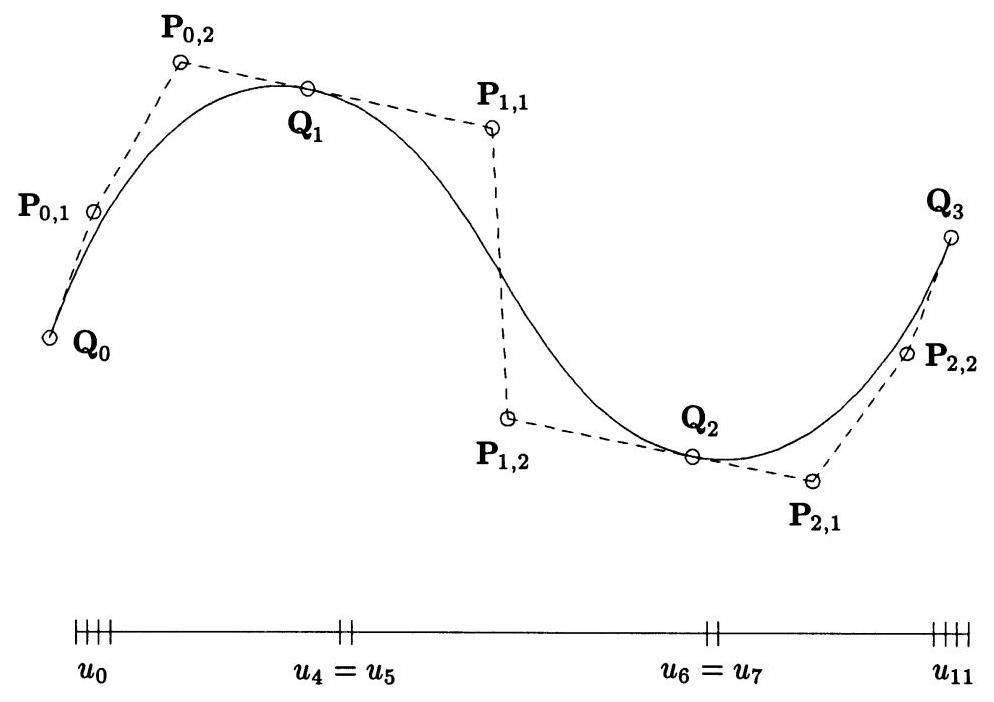
\includegraphics[max width=0.9\textwidth]{images/0193ba0d-ab19-7138-9798-cb281ce60de0_406_271_250_994_702_0.jpg}
\end{center}
\hspace*{3em} 

图 9.29. \({C}^{1}\) 局部三次曲线插值。

图 9.30 显示了使用该方法进行三次曲线插值的一个示例。曲线在对应于等间隔参数值的点上标记。图 9.31 是另一个使用与图 9.7 相同数据集的插值示例。注意共线点是如何通过直线三次段拟合的。


\subsection{局部双三次曲面插值}

也可以实现一个 \({C}^{\left( 1,1\right) }\) 连续的双三次局部曲面插值方案( \({C}^{1}\) 在 \(u\) 和 \(v\) 方向上均连续)。设 \(\left\{  {\mathbf{Q}}_{k,\ell }\right\}  ,k = 0,\ldots ,n\) 和 \(\ell  = 0,\ldots ,m\) 为一组数据点，设 \(\left\{  \left( {{\bar{u}}_{k},{\bar{v}}_{\ell }}\right) \right\}\) 为通过弦长平均计算的对应参数对(如算法 A9.3 所示)。以下方法生成满足条件的双三次曲面 \(\mathbf{S}\left( {u,v}\right)\) 。

\[
\mathbf{S}\left( {{\bar{u}}_{k},{\bar{v}}_{\ell }}\right)  = \mathop{\sum }\limits_{{i = 0}}^{{{2n} + 1}}\mathop{\sum }\limits_{{j = 0}}^{{{2m} + 1}}{N}_{i,3}\left( {\bar{u}}_{k}\right) {N}_{j,3}\left( {\bar{v}}_{\ell }\right) {\mathbf{P}}_{i,j} \tag{9.55}
\]

\begin{center}
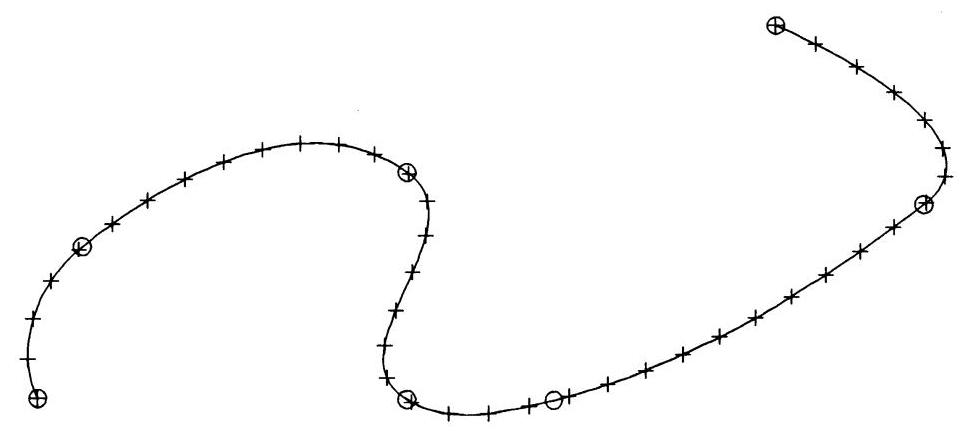
\includegraphics[max width=0.8\textwidth]{images/0193ba0d-ab19-7138-9798-cb281ce60de0_406_281_1597_966_432_0.jpg}
\end{center}
\hspace*{3em} 

图 9.30. 局部三次曲线插值的参数化；这些点是在等间隔参数值下计算的。

\begin{center}
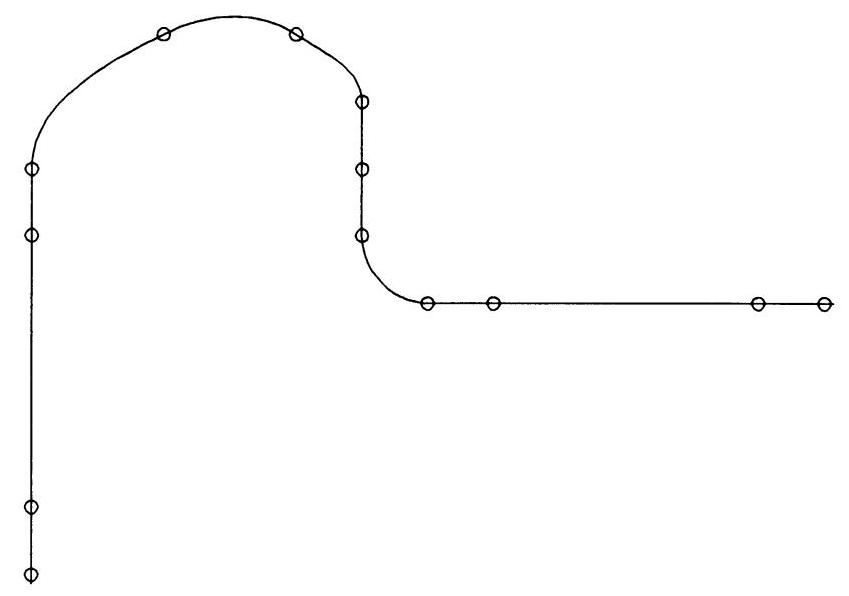
\includegraphics[max width=0.7\textwidth]{images/0193ba0d-ab19-7138-9798-cb281ce60de0_407_343_250_849_596_0.jpg}
\end{center}
\hspace*{3em} 

图 9.31. 对图 9.7 中数据的三次曲线插值；注意共线性是如何被保持的。

我们通过构造 \({nm}\) 双三次 Bézier 补丁来获得表面， \(\left\{  {{\mathbf{B}}_{k,\ell }\left( {u,v}\right) }\right\}\) ， \(k = 0,\ldots ,n - 1,\ell  = 0,\ldots ,m - 1\) ，其中 \({\mathbf{Q}}_{k,\ell },{\mathbf{Q}}_{k + 1,\ell },{\mathbf{Q}}_{k,\ell  + 1},{\mathbf{Q}}_{k + 1,\ell  + 1}\) 是补丁的角点，补丁在其边界处以 \({C}^{\left( 1,1\right) }\) 连续性连接。除了表面边界外，所有包含原始 \(\left\{  {\mathbf{Q}}_{k,\ell }\right\}\) 的控制点的行和列都被移除(见图 9.32b 和 9.32c)，最终的 B-spline 表面留下 \(\left( {{2n} + 2}\right) \left( {{2m} + 2}\right)\) 个控制点。节点向量为

\[
U = \left\{  {0,0,0,0,{\bar{u}}_{1},{\bar{u}}_{1},{\bar{u}}_{2},{\bar{u}}_{2},\ldots ,{\bar{u}}_{n - 1},{\bar{u}}_{n - 1},1,1,1,1}\right\}
\]

\[
V = \left\{  {0,0,0,0,{\bar{v}}_{1},{\bar{v}}_{1},{\bar{v}}_{2},{\bar{v}}_{2},\ldots ,{\bar{v}}_{m - 1},{\bar{v}}_{m - 1},1,1,1,1}\right\}   \tag{9.56}
\]

一个双三次 Bézier 补丁有 16 个控制点。12 个边界控制点是通过最初遍历 \(m + 1\) 行和 \(n + 1\) 列的数据并使用三次曲线插值方案获得的。该方案与之前详细描述的方案略有不同，因为我们已经有了参数 \(\left\{  \left( {{\bar{u}}_{k},{\bar{v}}_{\ell }}\right) \right\}\) 。请注意，这些参数必须提前计算，因为在张量积表面中，所有行(列)必须具有相同的参数化。因此，我们仍然可以在段的端点强制 \({C}^{1}\) 连续性，但无法在 Bézier 曲线段的中点强制相等的速度。更具体地说，设 \(\ell  = {\ell }_{0}\) 为固定，并考虑插值这些点的三次曲线

\begin{center}
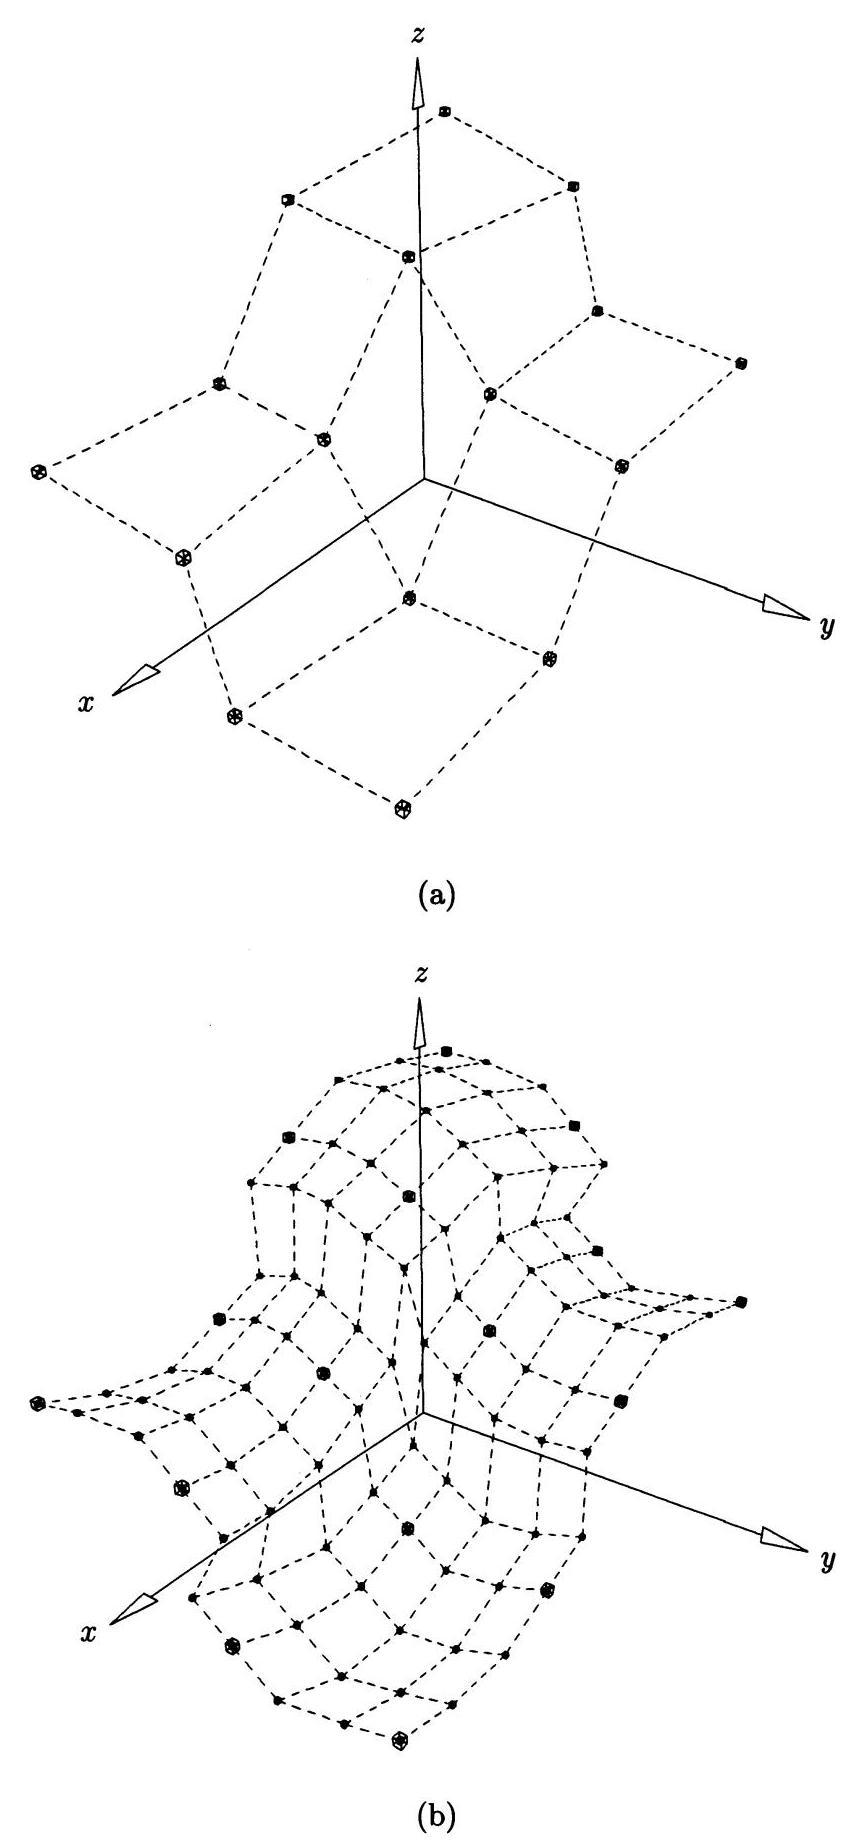
\includegraphics[max width=0.7\textwidth]{images/0193ba0d-ab19-7138-9798-cb281ce60de0_408_340_235_861_1841_0.jpg}
\end{center}
\hspace*{3em} 

图 9.32. \({C}^{\left( 1,1\right) }\) 局部双三次表面插值。(a) 数据集；(b) 插值的 Bézier 网格。

402 曲线和表面拟合 \({\mathbf{Q}}_{0,{\ell }_{0}},\ldots ,{\mathbf{Q}}_{n,{\ell }_{0}}\) 。设 \({r}_{{\ell }_{0}}\) 表示第 \({\ell }_{0}\) 行的总弦长。在每个点 \({\mathbf{Q}}_{k,{\ell }_{0}}\) 处，计算 \({\mathbf{T}}_{k,{\ell }_{0}}^{u}\) (在 \(u\) 方向上的单位切线)，如前所述(方程 [9.29]、[9.31] 和 [9.33])。然后，通过以下方式计算该行的内部 Bézier 点

\[
{\mathbf{P}}_{1,0}^{k,{\ell }_{0}} = {\mathbf{Q}}_{k,{\ell }_{0}} + a{\mathbf{T}}_{k,{\ell }_{0}}^{u}\;{\mathbf{P}}_{2,0}^{k,{\ell }_{0}} = {\mathbf{Q}}_{k + 1,{\ell }_{0}} - a{\mathbf{T}}_{k + 1,{\ell }_{0}}^{u} \tag{9.57}
\]

\begin{center}
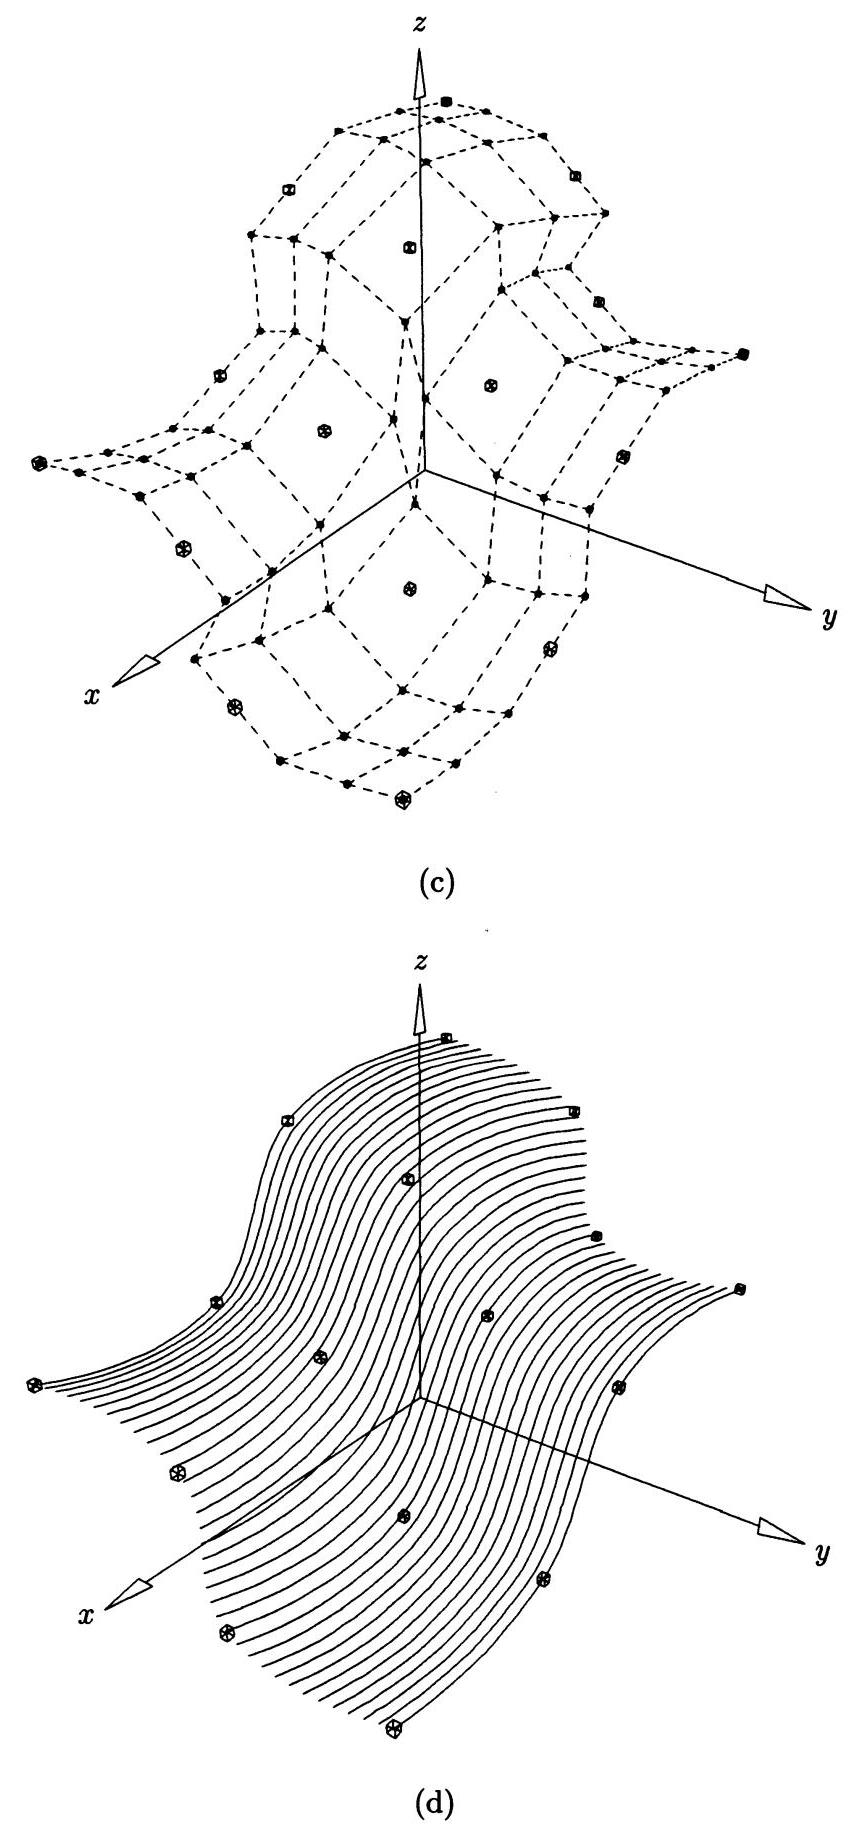
\includegraphics[max width=0.7\textwidth]{images/0193ba0d-ab19-7138-9798-cb281ce60de0_409_340_248_861_1824_0.jpg}
\end{center}
\hspace*{3em} 

图 9.32.(续)(c) 一个 B-spline 网(大立方体标记数据点，小立方体是 B-spline 控制点)；(d) 表面插值函数。

在哪里

\[
a = \frac{{r}_{{\ell }_{0}}\left( {{\bar{u}}_{k + 1} - {\bar{u}}_{k}}\right) }{3} = \frac{{r}_{{\ell }_{0}}\Delta {\bar{u}}_{k + 1}}{3}
\]

结果曲线是 \({C}^{1}\) 连续的，导数的大小在所有 \({\mathbf{Q}}_{k,{\ell }_{0}}\) 处等于 \({r}_{{\ell }_{0}}\) 。同样的技术应用于 \(n + 1\) 数据列。

现在需要计算每个 Bézier 补丁的四个内部控制点。这需要在每个 \({\mathbf{Q}}_{k,\ell }\) 处对混合偏导数 \({\mathbf{D}}_{k,\ell }^{uv}\) 的估计，以及方程 (3.24)(和其他三个角的类似公式)。我们基于三点贝塞尔方法(方程 [9.28]、[9.30] 和 [9.32])推导出 \({\mathbf{D}}_{k,\ell }^{uv}\) 的公式。设 \({r}_{\ell }\) 和 \({s}_{k}\) 表示第 \(\ell\) 行(第 k 列)的总弦长。那么

\[
{\mathbf{D}}_{k,\ell }^{u} = {r}_{\ell }{\mathbf{T}}_{k,\ell }^{u}\;{\mathbf{D}}_{k,\ell }^{v} = {s}_{k}{\mathbf{T}}_{k,\ell }^{v} \tag{9.58}
\]

然后设置

\[
{\mathbf{d}}_{k,\ell }^{vu} = \left( {1 - {\alpha }_{k}}\right) \frac{{\mathbf{D}}_{k,\ell }^{v} - {\mathbf{D}}_{k - 1,\ell }^{v}}{\Delta {\bar{u}}_{k}} + {\alpha }_{k}\frac{{\mathbf{D}}_{k + 1,\ell }^{v} - {\mathbf{D}}_{k,\ell }^{v}}{\Delta {\bar{u}}_{k + 1}}
\]

和

\[
{\mathbf{d}}_{k,\ell }^{uv} = \left( {1 - {\beta }_{\ell }}\right) \frac{{\mathbf{D}}_{k,\ell }^{u} - {\mathbf{D}}_{k,\ell  - 1}^{u}}{\Delta {\bar{v}}_{\ell }} + {\beta }_{\ell }\frac{{\mathbf{D}}_{k,\ell  + 1}^{u} - {\mathbf{D}}_{k,\ell }^{u}}{\Delta {\bar{v}}_{\ell  + 1}}
\]

与

\[
{\alpha }_{k} = \frac{\Delta {\bar{u}}_{k}}{\Delta {\bar{u}}_{k} + \Delta {\bar{u}}_{k + 1}}\;{\beta }_{\ell } = \frac{\Delta {\bar{v}}_{\ell }}{\Delta {\bar{v}}_{\ell } + \Delta {\bar{v}}_{\ell  + 1}}
\]

最后

\[
{\mathbf{D}}_{k,\ell }^{uv} = \frac{{\alpha }_{k}{\mathbf{d}}_{k,\ell }^{uv} + {\beta }_{\ell }{\mathbf{d}}_{k,\ell }^{vu}}{{\alpha }_{k} + {\beta }_{\ell }} \tag{9.59}
\]

在边界上必须使用适当的结束公式(方程 [9.32])。现在使用方程 (9.59) 和 (3.24) 计算 \(\left( {k,\ell }\right)\) 补丁的四个内部控制点。

\[
{\mathbf{P}}_{1,1}^{k,\ell } = \gamma {\mathbf{D}}_{k,\ell }^{uv} + {\mathbf{P}}_{0,1}^{k,\ell } + {\mathbf{P}}_{1,0}^{k,\ell } - {\mathbf{P}}_{0,0}^{k,\ell }
\]

\[
{\mathbf{P}}_{2,1}^{k,\ell } =  - \gamma {\mathbf{D}}_{k + 1,\ell }^{uv} + {\mathbf{P}}_{3,1}^{k,\ell } - {\mathbf{P}}_{3,0}^{k,\ell } + {\mathbf{P}}_{2,0}^{k,\ell }
\]

\[
{\mathbf{P}}_{1,2}^{k,\ell } =  - \gamma {\mathbf{D}}_{k,\ell  + 1}^{uv} + {\mathbf{P}}_{1,3}^{k,\ell } - {\mathbf{P}}_{0,3}^{k,\ell } + {\mathbf{P}}_{0,2}^{k,\ell }
\]

\[
{\mathbf{P}}_{2,2}^{k,\ell } = \gamma {\mathbf{D}}_{k + 1,\ell  + 1}^{uv} + {\mathbf{P}}_{2,3}^{k,\ell } + {\mathbf{P}}_{3,2}^{k,\ell } - {\mathbf{P}}_{3,3}^{k,\ell }
\]

在哪里

\[
\gamma  = \frac{\Delta {\bar{u}}_{k + 1}\Delta {\bar{v}}_{\ell  + 1}}{9}
\]

现在我们用一个算法进行总结。为了提高效率，事件的顺序与此处详细描述的略有不同。该算法需要局部数组: \({td}\left\lbrack  {n + 1}\right\rbrack  \left\lbrack  {m + 1}\right\rbrack  \left\lbrack  3\right\rbrack\) ，包含 \({\mathbf{T}}_{k,\ell }^{u},{\mathbf{T}}_{k,\ell }^{v}\) 和 \({\mathbf{D}}_{k,\ell }^{uv}\) ；ub \(\left\lbrack  {n + 1}\right\rbrack\) 和 \({vb}\left\lbrack  {m + 1}\right\rbrack\) ，包含参数值；以及 \(r\left\lbrack  {m + 1}\right\rbrack\) 和 \(s\left\lbrack  {n + 1}\right\rbrack\) ，分别存储行和列的总弦长。

\HRule

ALGORITHM A9.5

\hspace*{2em} LocalSurfInterp(n, m, Q, U, V, P)

\hspace*{4em} \{ /* Local surface interpolation */

\hspace*{4em} \{ /* through \(\left( {n + 1}\right) \left( {m + 1}\right)\) points */

\hspace*{7em} /* Input: n, m, Q */

\hspace*{7em} /* Output: U, V, P */

\hspace*{4em} total \(= {0.0}\) ; /* get ub[], \(r\) [] and u direction tangents \(*\) /

\hspace*{4em} for (k=0; k<=n; k++) ub[k] = 0.0;

\hspace*{4em} for (l=0; l<=m; l++)

\hspace*{6em} \{

\hspace*{6em} Compute and load \({\mathbf{T}}_{0,\ell }^{u}\) into td[0][1][0];

\hspace*{6em} r[1] = 0.0 ;

\hspace*{6em} for (k=1; k<=n; k++)

\hspace*{8em} \{

\hspace*{8em} Compute and load \({\mathbf{T}}_{k,\ell }^{u}\) into \({td}\left\lbrack  k\right\rbrack  \left\lbrack  1\right\rbrack  \left\lbrack  0\right\rbrack\)

\hspace*{13em} /* Eqs. (9.31) and (9.33) */

\hspace*{8em} \(\mathrm{d} = \left| {{\mathbf{Q}}_{k,\ell } - {\mathbf{Q}}_{k - 1,\ell }}\right| ;\)

\hspace*{8em} \({ub}\left\lbrack  k\right\rbrack   = {ub}\left\lbrack  k\right\rbrack   + d\) ;

\hspace*{8em} r[l] = r[l]+d;

\hspace*{8em} \}

\hspace*{6em} total = total + r[l];

\hspace*{6em} \}

\hspace*{4em} for \(\left( {k = 1;k < n;k +  + }\right) \;{ub}\left\lbrack  k\right\rbrack   = {ub}\left\lbrack  {k - 1}\right\rbrack   + {ub}\left\lbrack  k\right\rbrack  /\) total;

\hspace*{4em} ub[n] = 1.0;

\hspace*{4em} total \(= {0.0}\) ; /* get vb[], \(s\) [] and \(v\) direction tangents \(*\) /

\hspace*{4em} for (l=0; l<=m; l++) vb[l] = 0.0;

\hspace*{4em} for (k=0; k<=n; k++)

\hspace*{6em} \{

\hspace*{6em} Compute and load \({\mathbf{T}}_{k,0}^{v}\) into \(\operatorname{td}\left\lbrack  \mathrm{k}\right\rbrack  \left\lbrack  0\right\rbrack  \left\lbrack  1\right\rbrack\) ;

\hspace*{6em} s[k] = 0.0 ;

\hspace*{6em} for (l=1; l<=m; l++)

\hspace*{8em} \{

\hspace*{8em} Compute and load \({\mathbf{T}}_{k,\ell }^{v}\) into \({td}\left\lbrack  k\right\rbrack  \left\lbrack  1\right\rbrack  \left\lbrack  1\right\rbrack\)

\hspace*{13em} /* Eqs. (9.31) and (9.33) */

\hspace*{8em} \(\mathrm{d} = \left| {{\mathbf{Q}}_{k,\ell } - {\mathbf{Q}}_{k,\ell  - 1}}\right| ;\)

\hspace*{8em} vb[l] = vb[l]+d;

\hspace*{8em} \(s\left\lbrack  k\right\rbrack   = s\left\lbrack  k\right\rbrack   + d;\)

\hspace*{8em} \}

\hspace*{6em} total = total + s[k];

\hspace*{6em} \}

for \(\left( {l = 1;l < m;l +  + }\right) \;{vb}\left\lbrack  l\right\rbrack   = {vb}\left\lbrack  {l - 1}\right\rbrack   + {vb}\left\lbrack  l\right\rbrack  /\) total;

vb[m] = 1.0;

Load the U knot vector;

Load the V knot vector;

Compute all Bézier control points along each row and

\hspace*{3em} column of data points.

for \(\left( {k = 0;k <  = n;k +  + }\right)\)

\hspace*{2em} for (l=0; l<=m; l++)

\hspace*{3em} \{

\hspace*{3em} Compute the \({\mathbf{D}}_{k,\ell }^{uv}\) by Eq. (9.59) and load into \({td}\left\lbrack  k\right\rbrack  \left\lbrack  1\right\rbrack  \left\lbrack  2\right\rbrack\) .

\hspace*{3em} \}

for \(\left( {k = 0;k < n;k +  + }\right)\)

\hspace*{1em} for (l=0; l<m; l++)

\hspace*{3em} \{

\hspace*{3em} Compute the four inner control points of the(k, l)th

\hspace*{5em} Bezier patch and load them into \(P\) .

\hspace*{3em} \}

Load the NURBS control points by discarding Bézier points

\hspace*{3em} along inner rows and columns. /* Figure 9.32c */

\}

\HRule

图 9.32 显示了表面构造过程。在图 9.32a 中，数据点用小立方体标记。图 9.32b 说明了 Bézier 补丁的控制点。沿内行和内列消除 Bézier 点会产生图 9.32c 所示的 NURBS 表面控制网。表面在图 9.32d 中显示。

该插值方案可以轻松生成闭合的 \({C}^{\left( 1,1\right) }\) 连续表面。图 9.33a 和 \({9.33}\mathrm{\;b}\) 显示了一个表面插值的示例，其中数据指示在一个方向上是闭合的表面。在图 9.34a 和 \({9.34}\mathrm{\;b}\) 中，表面在两个方向上都是闭合的(类似于环形插值)。该方法的一个优良特性是，当数据点指示平面性时，会生成平坦(平面)补丁。图 9.35a 和 9.35b 显示了这一点的一个示例。

当数据不均匀分布时，获得令人满意的表面比获得曲线更为困难。图 \({9.36}\mathrm{a}\) 和 \({9.36}\mathrm{\;b}\) 显示了对非常不均匀分布数据的插值。尽管表面并不特别令人满意，但使用前一节的全局方法得到的结果并没有太大不同。



\section{全局逼近}

逼近比插值更为困难。在插值中，控制点的数量由所选的次数和数据项的数量自动确定，节点放置也很简单，并且没有需要检查的曲线或表面误差。在逼近中，曲线/表面误差界限 \(E\) 与要拟合的数据一起输入。通常事先并不知道需要多少个控制点才能获得所需的精度 \(E\) ，并且 406 曲线和表面拟合

\begin{center}
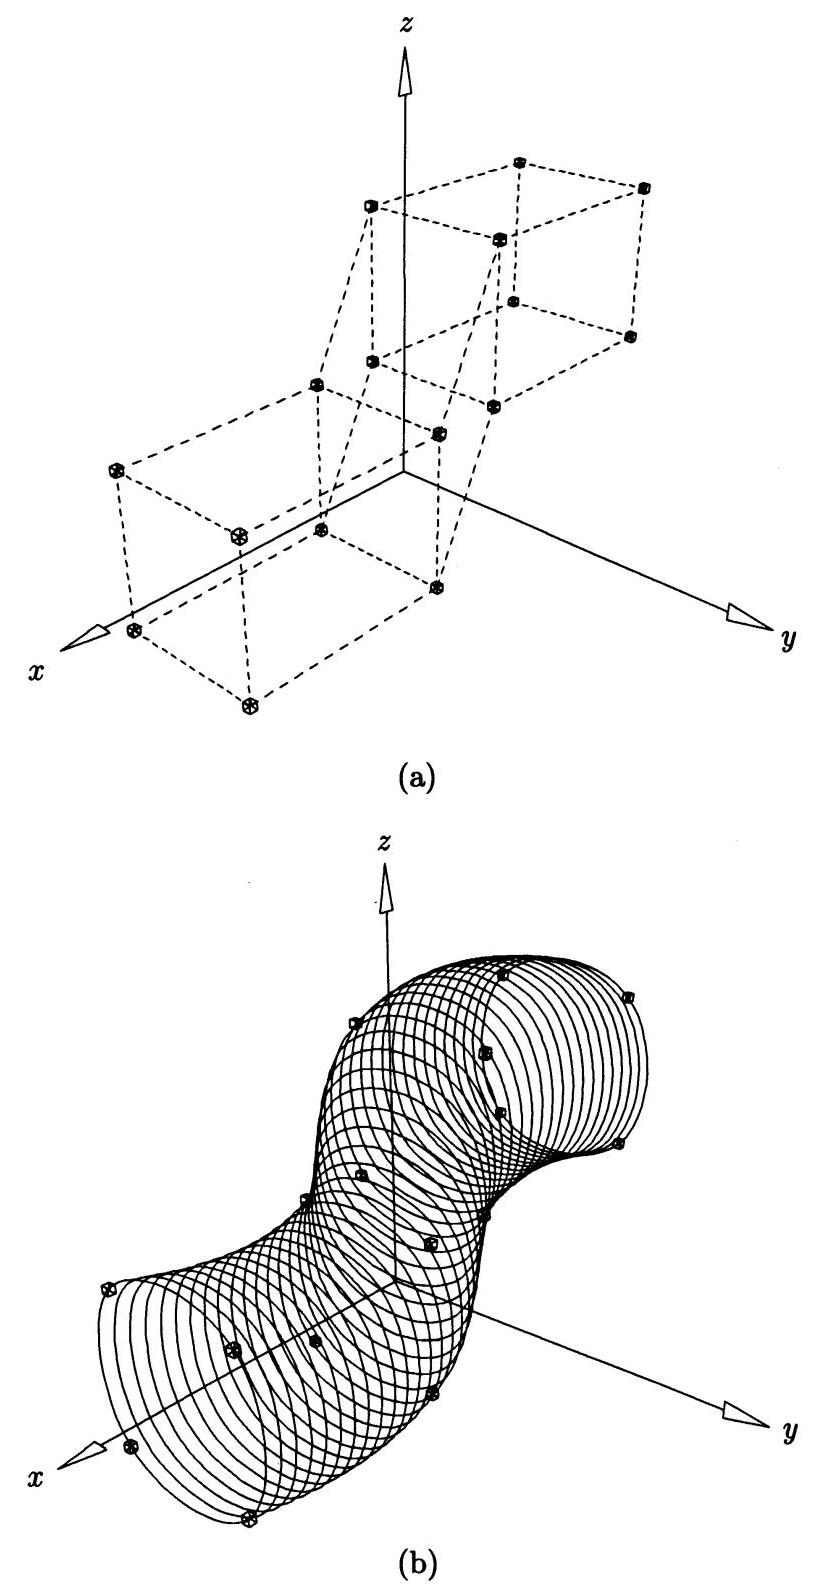
\includegraphics[max width=0.7\textwidth]{images/0193ba0d-ab19-7138-9798-cb281ce60de0_413_358_241_824_1589_0.jpg}
\end{center}
\hspace*{3em} 

图 9.33. 使用局部双三次曲面插值的表面插值示例。 (a) 数据点; (b) 插值表面。

因此，近似方法通常是迭代的。粗略来说，全局方法有两种进行方式:

1a. 从最小或少量控制点开始；

b. 使用全局拟合方法将近似曲线或表面拟合到数据上；

\begin{center}
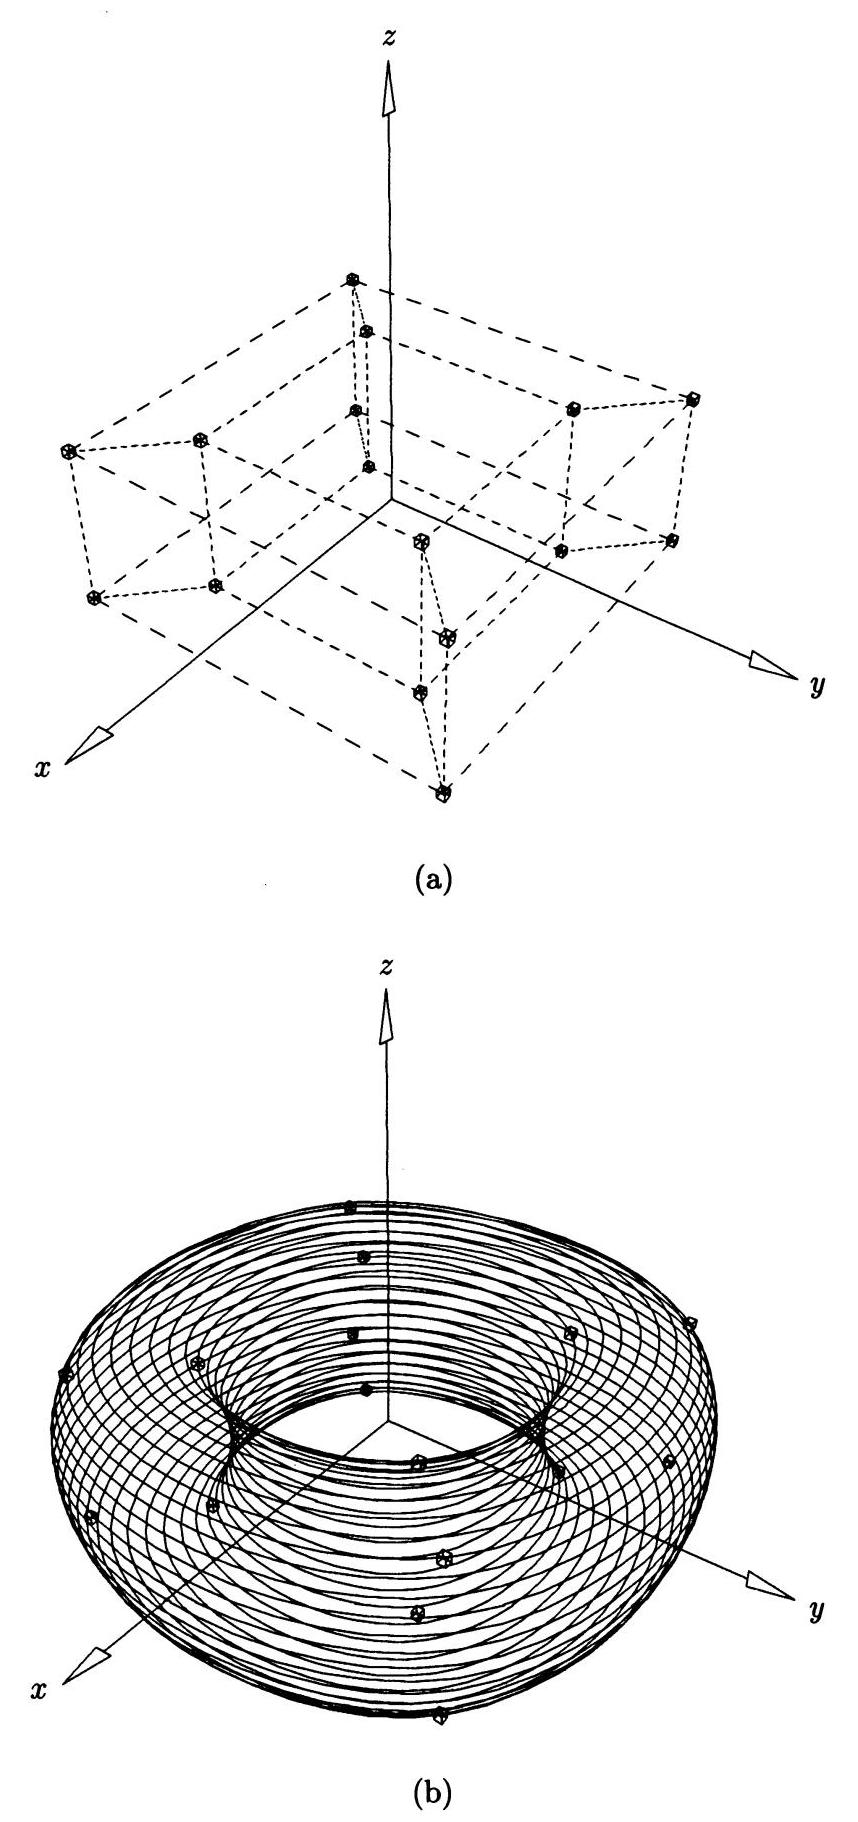
\includegraphics[max width=0.7\textwidth]{images/0193ba0d-ab19-7138-9798-cb281ce60de0_414_341_238_858_1822_0.jpg}
\end{center}
\hspace*{3em} 

图 9.34. 使用局部双三次曲面插值的表面插值示例。 (a) 数据点; (b) 插值表面。

408 曲线和表面拟合

\begin{center}
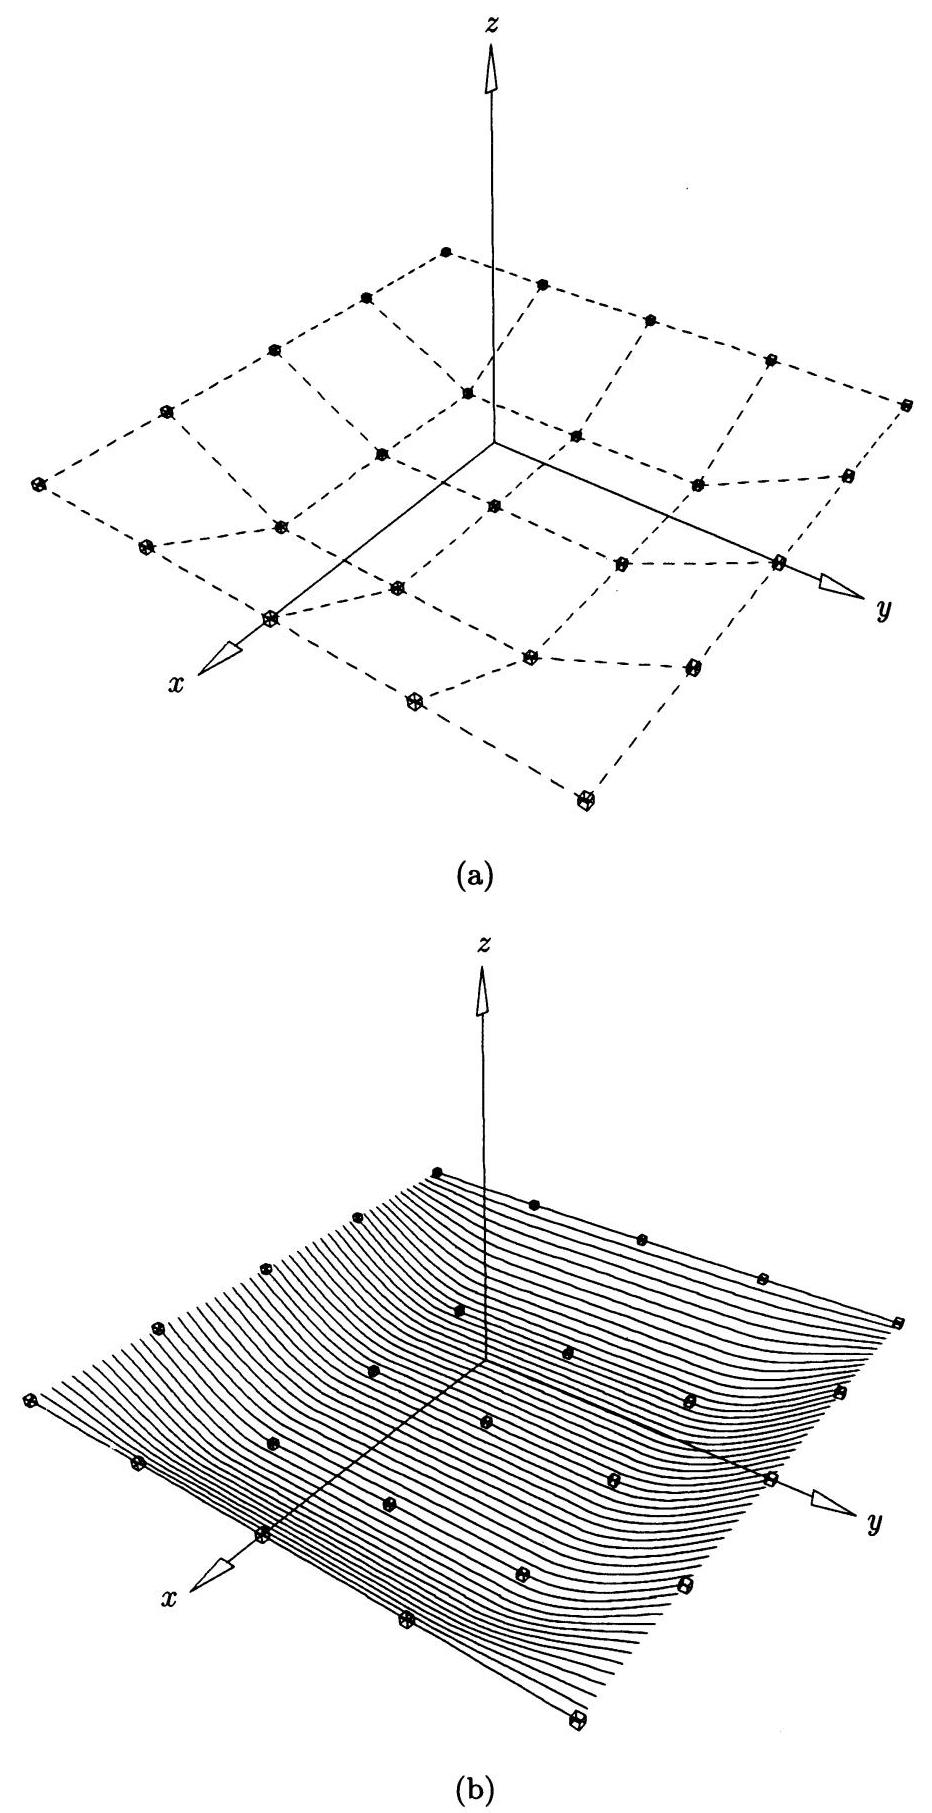
\includegraphics[max width=0.8\textwidth]{images/0193ba0d-ab19-7138-9798-cb281ce60de0_415_301_242_932_1813_0.jpg}
\end{center}
\hspace*{3em} 

图 9.35. 使用局部双三次曲面插值的表面插值示例。 (a) 数据点; (b) 插值表面。

\begin{center}
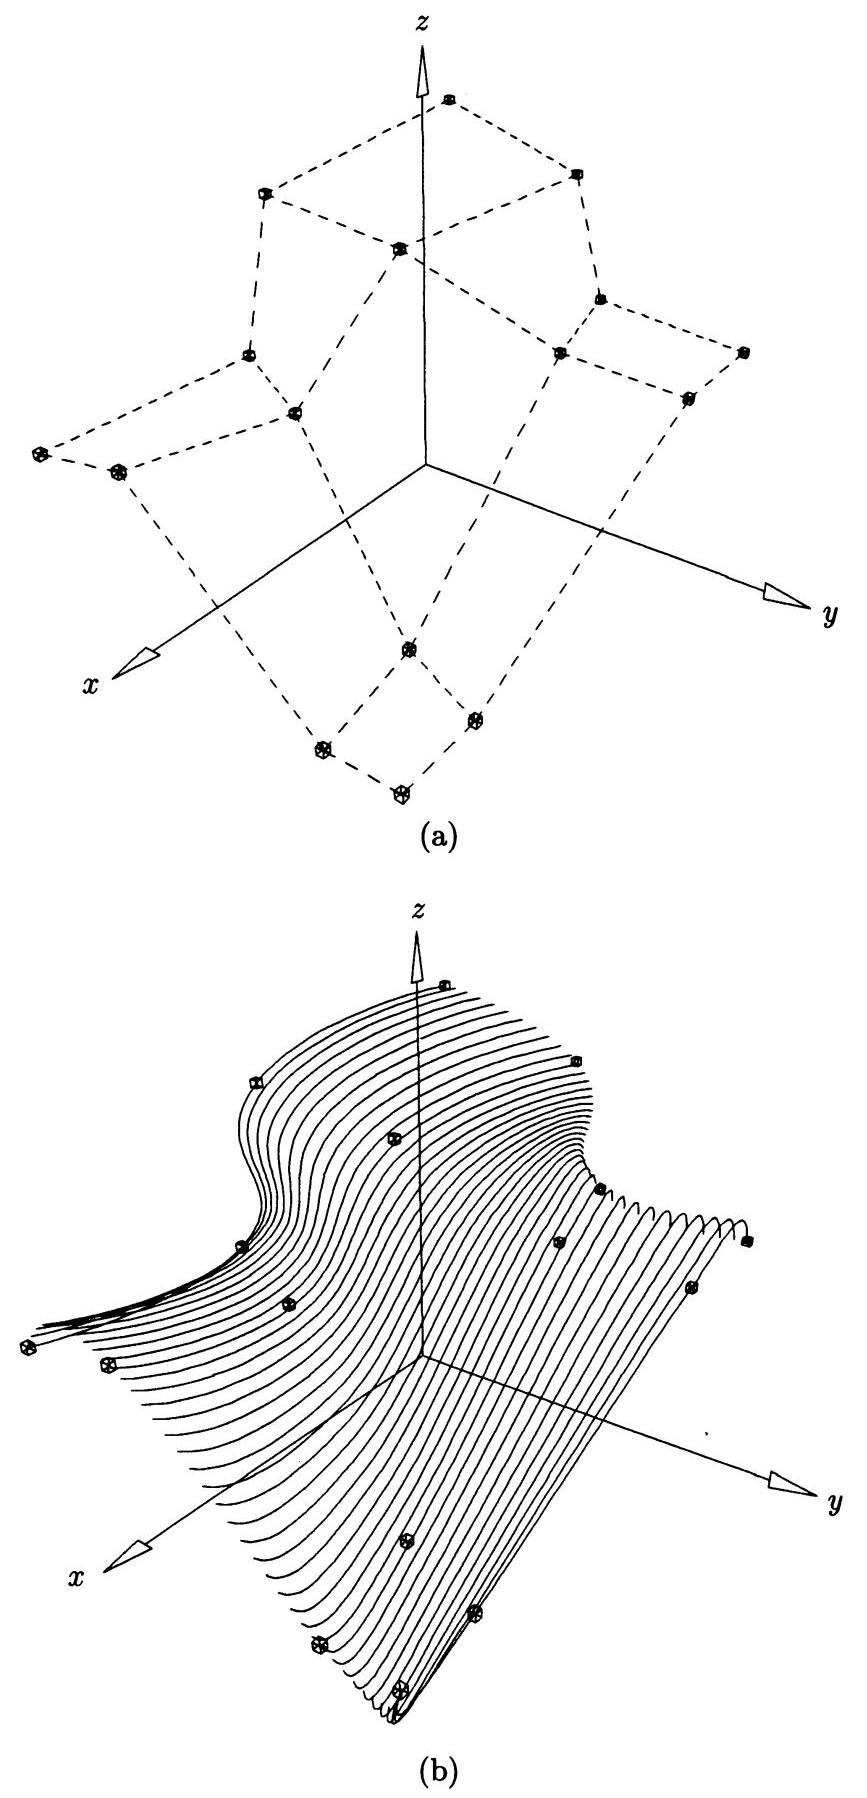
\includegraphics[max width=0.7\textwidth]{images/0193ba0d-ab19-7138-9798-cb281ce60de0_416_336_243_867_1798_0.jpg}
\end{center}
\hspace*{3em} 

图 9.36. 使用局部双三次曲面插值的表面插值示例。 (a) 数据点; (b) 插值表面。

c. 检查曲线/表面与数据的偏差；

d. 如果偏差处处小于 \(E\) ，则返回；否则增加控制点的数量并返回到步骤 1(b)。

2a. 从最大或“多个”控制点开始，足够使得第一次近似满足 \(E\) ；

b. 使用全局方法将曲线/表面拟合到数据上；

c. 检查偏差 \(E\) 是否在所有地方都满足；

d. 如果 \(E\) 不再满足，返回之前的曲线或表面，否则减少控制点的数量并返回到步骤 2(b)。

我们在第 9.4.4 节中回到这两种方法，特别是我们给出第二种类型的示例。显然，近似的成本也高于插值。需要多次拟合，并且偏差检查可能会很昂贵。

这两种方法的一个核心要素是，给定固定数量的控制点，例如 \(n\) ，我们将一个近似曲线(表面)拟合到数据上。有很多方法可以做到这一点。例如，可以建立一个非线性优化问题，其中控制点、参数 \(\left( {\bar{u}}_{k}\right)\) 、节点，甚至权重都是未知数。需要最小化的目标函数必须以某种方式衡量误差，例如，最小二乘法或最大偏差(例如，见 [Laur93])。在第 9.4.1-9.4.3 节中，我们介绍了曲线和表面拟合方法，其中固定数量的控制点是唯一的未知数，并使用线性最小二乘技术进行求解。



\subsection{最小二乘曲线逼近}

为了避免非线性问题，我们将权重设置为 1，并预计算参数和节点的值。然后我们建立并求解未知控制点的(唯一)线性最小二乘问题。我们从对点数据的简单曲线拟合开始。假设 \(p \geq  1,n \geq  p\) 和 \({\mathbf{Q}}_{0},\ldots ,{\mathbf{Q}}_{m}\left( {m > n}\right)\) 已知。我们寻求一个 \(p\) 次非有理曲线

\[
\mathbf{C}\left( u\right)  = \mathop{\sum }\limits_{{i = 0}}^{n}{N}_{i,p}\left( u\right) {\mathbf{P}}_{i}\;u \in  \left\lbrack  {0,1}\right\rbrack   \tag{9.61}
\]

满足以下条件:

\begin{itemize}
\item \({\mathbf{Q}}_{0} = \mathbf{C}\left( 0\right)\) 和 \({\mathbf{Q}}_{m} = \mathbf{C}\left( 1\right)\) ；
\end{itemize}

\begin{itemize}
\item 剩余的 \({\mathbf{Q}}_{k}\) 在最小二乘意义下被近似，即。
\end{itemize}

\[
\mathop{\sum }\limits_{{k = 1}}^{{m - 1}}{\left| {\mathbf{Q}}_{k} - \mathbf{C}\left( {\bar{u}}_{k}\right) \right| }^{2} \tag{9.62}
\]

是相对于 \(n + 1\) 变量的最小值， \({\mathbf{P}}_{i}\) ； \(\left\{  {\bar{u}}_{k}\right\}\) 是预计算的参数值。

我们强调，结果曲线通常并不精确地通过 \({\mathbf{Q}}_{k}\) ，而且 \(\mathbf{C}\left( {\bar{u}}_{k}\right)\) 不是 \(\mathbf{C}\left( u\right)\) 上离 \({\mathbf{Q}}_{k}\) 最近的点。设

\[
{\mathbf{R}}_{k} = {\mathbf{Q}}_{k} - {N}_{0,p}\left( {\bar{u}}_{k}\right) {\mathbf{Q}}_{0} - {N}_{n,p}\left( {\bar{u}}_{k}\right) {\mathbf{Q}}_{m}\;k = 1,\ldots ,m - 1 \tag{9.63}
\]

然后设定

\[
f = \mathop{\sum }\limits_{{k = 1}}^{{m - 1}}{\left| {\mathbf{Q}}_{k} - \mathbf{C}\left( {\bar{u}}_{k}\right) \right| }^{2} = \mathop{\sum }\limits_{{k = 1}}^{{m - 1}}{\left| {\mathbf{R}}_{k} - \mathop{\sum }\limits_{{i = 1}}^{{n - 1}}{N}_{i,p}\left( {\bar{u}}_{k}\right) {\mathbf{P}}_{i}\right| }^{2}
\]

\[
= \mathop{\sum }\limits_{{k = 1}}^{{m - 1}}\left( {{\mathbf{R}}_{k} - \mathop{\sum }\limits_{{i = 1}}^{{n - 1}}{N}_{i,p}\left( {\bar{u}}_{k}\right) {\mathbf{P}}_{i}}\right)  \cdot  \left( {{\mathbf{R}}_{k} - \mathop{\sum }\limits_{{i = 1}}^{{n - 1}}{N}_{i,p}\left( {\bar{u}}_{k}\right) {\mathbf{P}}_{i}}\right)
\]

\[
= \mathop{\sum }\limits_{{k = 1}}^{{m - 1}}\left\lbrack  {{\mathbf{R}}_{k} \cdot  {\mathbf{R}}_{k} - 2\mathop{\sum }\limits_{{i = 1}}^{{n - 1}}{N}_{i,p}\left( {\bar{u}}_{k}\right) \left( {{\mathbf{R}}_{k} \cdot  {\mathbf{P}}_{i}}\right) }\right.
\]

\[
\left. {+\left( {\mathop{\sum }\limits_{{i = 1}}^{{n - 1}}{N}_{i,p}\left( {\bar{u}}_{k}\right) {\mathbf{P}}_{i}}\right)  \cdot  \left( {\mathop{\sum }\limits_{{i = 1}}^{{n - 1}}{N}_{i,p}\left( {\bar{u}}_{k}\right) {\mathbf{P}}_{i}}\right) }\right\rbrack
\]

\(f\) 是 \(n - 1\) 变量的标量值函数， \({\mathbf{P}}_{1},\ldots ,{\mathbf{P}}_{n - 1}\) 。现在我们应用线性最小二乘拟合的标准技术 [DeBo78; Vand83; Lanc86]；为了最小化 \(f\) ，我们将 \(f\) 关于 \(n - 1\) 点的导数， \({\mathbf{P}}_{\ell }\) ，设为零。 \(\ell\) 阶导数是

\[
\frac{\partial f}{\partial {\mathbf{P}}_{\ell }} = \mathop{\sum }\limits_{{k = 1}}^{{m - 1}}\left( {-2{N}_{\ell ,p}\left( {\bar{u}}_{k}\right) {\mathbf{R}}_{k} + 2{N}_{\ell ,p}\left( {\bar{u}}_{k}\right) \mathop{\sum }\limits_{{i = 1}}^{{n - 1}}{N}_{i,p}\left( {\bar{u}}_{k}\right) {\mathbf{P}}_{i}}\right)
\]

这意味着

\[
- \mathop{\sum }\limits_{{k = 1}}^{{m - 1}}{N}_{\ell ,p}\left( {\bar{u}}_{k}\right) {\mathbf{R}}_{k} + \mathop{\sum }\limits_{{k = 1}}^{{m - 1}}\mathop{\sum }\limits_{{i = 1}}^{{n - 1}}{N}_{\ell ,p}\left( {\bar{u}}_{k}\right) {N}_{i,p}\left( {\bar{u}}_{k}\right) {\mathbf{P}}_{i} = 0
\]

由此可得

\[
\mathop{\sum }\limits_{{i = 1}}^{{n - 1}}\left( {\mathop{\sum }\limits_{{k = 1}}^{{m - 1}}{N}_{\ell ,p}\left( {\bar{u}}_{k}\right) {N}_{i,p}\left( {\bar{u}}_{k}\right) }\right) {\mathbf{P}}_{i} = \mathop{\sum }\limits_{{k = 1}}^{{m - 1}}{N}_{\ell ,p}\left( {\bar{u}}_{k}\right) {\mathbf{R}}_{k} \tag{9.64}
\]

方程 (9.64) 是一个关于未知数 \({\mathbf{P}}_{1},\ldots ,{\mathbf{P}}_{n - 1}\) 的线性方程。令 \(\ell  = 1,\ldots ,n - 1\) 得到 \(n - 1\) 个方程的系统，其中有 \(n - 1\) 个未知数

\[
\left( {{N}^{T}N}\right) \mathbf{P} = \mathbf{R} \tag{9.65}
\]

其中 \(N\) 是标量的 \(\left( {m - 1}\right)  \times  \left( {n - 1}\right)\) 矩阵

\[
N = \left\lbrack  \begin{matrix} {N}_{1,p}\left( {\bar{u}}_{1}\right) & \cdots & {N}_{n - 1,p}\left( {\bar{u}}_{1}\right) \\  \vdots &  \ddots  & \vdots \\  {N}_{1,p}\left( {\bar{u}}_{m - 1}\right) & \cdots & {N}_{n - 1,p}\left( {\bar{u}}_{m - 1}\right)  \end{matrix}\right\rbrack   \tag{9.66}
\]

\(\mathbf{R}\) 是 \(n - 1\) 点的向量

\[
\mathbf{R} = \left\lbrack  \begin{matrix} {N}_{1,p}\left( {\bar{u}}_{1}\right) {\mathbf{R}}_{1} + \cdots  + {N}_{1,p}\left( {\bar{u}}_{m - 1}\right) {\mathbf{R}}_{m - 1} \\  \vdots \\  {N}_{n - 1,p}\left( {\bar{u}}_{1}\right) {\mathbf{R}}_{1} + \cdots  + {N}_{n - 1,p}\left( {\bar{u}}_{m - 1}\right) {\mathbf{R}}_{m - 1} \end{matrix}\right\rbrack   \tag{9.67}
\]

和

\[
\mathbf{P} = \left\lbrack  \begin{matrix} {\mathbf{P}}_{1} \\  \vdots \\  {\mathbf{P}}_{n - 1} \end{matrix}\right\rbrack
\]

请注意，方程(9.65)是一个系数矩阵，具有三个右侧和三组未知数(x，y，z坐标)。为了建立方程(9.66)和(9.67)，需要一个节点向量 \(U = \left\{  {{u}_{0},\ldots ,{u}_{r}}\right\}\) 和参数 \(\left\{  {\bar{u}}_{k}\right\}\) 。可以使用方程(9.5)计算 \(\left\{  {\bar{u}}_{k}\right\}\) 。节点的放置应反映 \(\left\{  {\bar{u}}_{k}\right\}\) 的分布。如果 \(d\) 是一个正实数，则用 \(i = \operatorname{int}\left( d\right)\) 表示最大的整数，使得 \(i \leq  d\) 。我们需要总共 \(n + p + 2\) 个节点；其中有 \(n - p\) 个内部节点，以及 \(n - p + 1\) 个内部节点跨度。让

\[
d = \frac{m + 1}{n - p + 1} \tag{9.68}
\]

然后通过以下方式定义内部节点

\[
i = \operatorname{int}\left( {jd}\right) \;\alpha  = {jd} - i
\]

\[
{u}_{p + j} = \left( {1 - \alpha }\right) {\bar{u}}_{i - 1} + \alpha {\bar{u}}_{i}\;j = 1,\ldots ,n - p \tag{9.69}
\]

方程 (9.69) 保证每个节点区间至少包含一个 \({\bar{u}}_{k}\) ，在此条件下，deBoor [DeBo78] 表明方程 (9.65) 中的矩阵 \(\left( {{N}^{T}N}\right)\) 是正定且良好条件的。它可以通过高斯消元法解决，无需主元选择。此外， \(\left( {{N}^{T}N}\right)\) 的半带宽小于 \(p + 1\) (如果 \({N}_{i,j}\) 是第 \(i\) 行、第 \(j\) 列的元素，则 \({N}_{i,j} = 0\) 如果 \(\left| {i - j}\right|  > p\) )。最后，关于实现，注意矩阵 \(N\) (方程 [9.66])可能非常大，并且大多数元素为零；在某些应用中， \(m = {1000}\) 和 \(n = {100}\) 并不少见。因此，实现者可能希望开发一种存储方案，仅存储 \(N\) 的非零元素。一旦计算出 \(\left( {{N}^{T}N}\right)\) 和 \(\mathbf{R}\) (方程 [9.67])，可以释放 \(N\) 。类似地，仅应存储 \(\left( {{N}^{T}N}\right)\) 的非零带。

图 \({9.37}\mathrm{a} - {9.37}\mathrm{c}\) 显示了简单最小二乘曲线拟合的示例。在图 9.37a 中指定了七个控制点。图 9.37b 显示了九个控制点的拟合，而图 9.37c 描绘了十一个控制点的拟合。注意，从距离的角度来看，随着控制点数量的增加，近似效果有所改善。然而，当控制点的数量接近数据点的数量时，如果数据存在噪声或不必要的波动，可能会出现不理想的形状。

\begin{center}
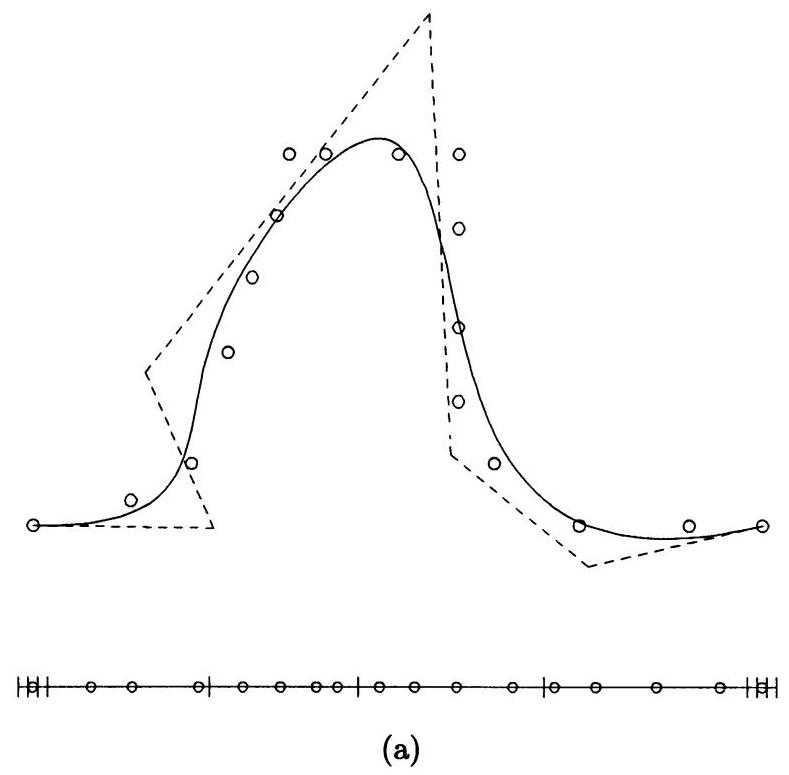
\includegraphics[max width=0.7\textwidth]{images/0193ba0d-ab19-7138-9798-cb281ce60de0_420_374_267_789_775_0.jpg}
\end{center}
\hspace*{3em} 

图 9.37. 全局曲线拟合。(a) 七个控制点；(b) 九个控制点；(c) 十一个控制点。


\subsection{加权和约束最小二乘曲线拟合}

现在我们提出一种非常通用的加权约束最小二乘曲线拟合方法。这是对Smith等人算法的NURBS适应 [Smit74]。设 \(\left\{  {\mathbf{Q}}_{i}\right\}  ,i = 0,\ldots ,r\) 为要近似的点。可选地，可以指定任意 \({\mathbf{Q}}_{i}\) 处的第一导数 \({\mathbf{D}}_{i}\) 。设 \(\left\{  {\mathbf{D}}_{i\left( j\right) }\right\}  ,j = 0,\ldots ,s\) 为导数集合； \(- 1 \leq  s \leq  r\) ，其中 \(s =  - 1\) 表示未指定导数。此外，任何 \({\mathbf{Q}}_{i}\) 或 \({\mathbf{D}}_{i\left( j\right) }\) 都可以被约束(精确插值)。我们将 \(\left\{  {\mathbf{Q}}_{i}\right\}\) 和 \(\left\{  {\mathbf{D}}_{i\left( j\right) }\right\}\) 分为无约束和有约束集合。用 \({\mathbf{Q}}_{i\left( 0\right) }^{u},\ldots ,{\mathbf{Q}}_{i\left( {r}_{u}\right) }^{u}\) 和 \({\mathbf{D}}_{i\left( 0\right) }^{u},\ldots ,{\mathbf{D}}_{i\left( {s}_{u}\right) }^{u}\) 表示无约束项，用 \({\mathbf{Q}}_{i\left( 0\right) }^{c},\ldots ,{\mathbf{Q}}_{i\left( {r}_{c}\right) }^{c}\) 和 \({\mathbf{D}}_{i\left( 0\right) }^{c},\ldots ,{\mathbf{D}}_{i\left( {s}_{c}\right) }^{c}\) 表示有约束项 \(\left( {{s}_{u},{s}_{c}}\right.\) ，或 \({r}_{c}\) 等于-1表示没有与此索引对应的数据。注意 \(r = {r}_{u} + {r}_{c} + 1\) 和 \(s = {s}_{u} + {s}_{c} + 1\) 。我们还允许为每个无约束项分配一个正权重，因此我们有 \({w}_{i\left( 0\right) }^{q},\ldots ,{w}_{i\left( {r}_{u}\right) }^{q}\) 和 \({w}_{i\left( 0\right) }^{d},\ldots ,{w}_{i\left( {s}_{u}\right) }^{d}\)  \(\left( {{w}_{i}^{q},{w}_{i}^{d} > 0}\right) .\) 。这些权重允许对每个数据项相对于其邻居的“紧密度”施加额外影响。 \({w}_{i}^{q},{w}_{i}^{d} = 1\) 是默认值。增加权重会增加对该项的近似紧密度，而减少权重则会放松对该项的近似。请注意，这些权重与NURBS意义上的权重无关。

现在设 \({m}_{u} = {r}_{u} + {s}_{u} + 1\) 和 \({m}_{c} = {r}_{c} + {s}_{c} + 1\) 。我们希望在最小二乘意义上近似无约束数据，并插值有约束数据

414 曲线和曲面拟合数据与一个 \(p\) 次非理性曲线 \(\mathbf{C}\left( u\right)\) ，具有 \(n + 1\) 个控制点。下一个算法要求

\[
{m}_{c} < n\;{m}_{c} + n < {m}_{u} + 1 \tag{9.70}
\]

\begin{center}
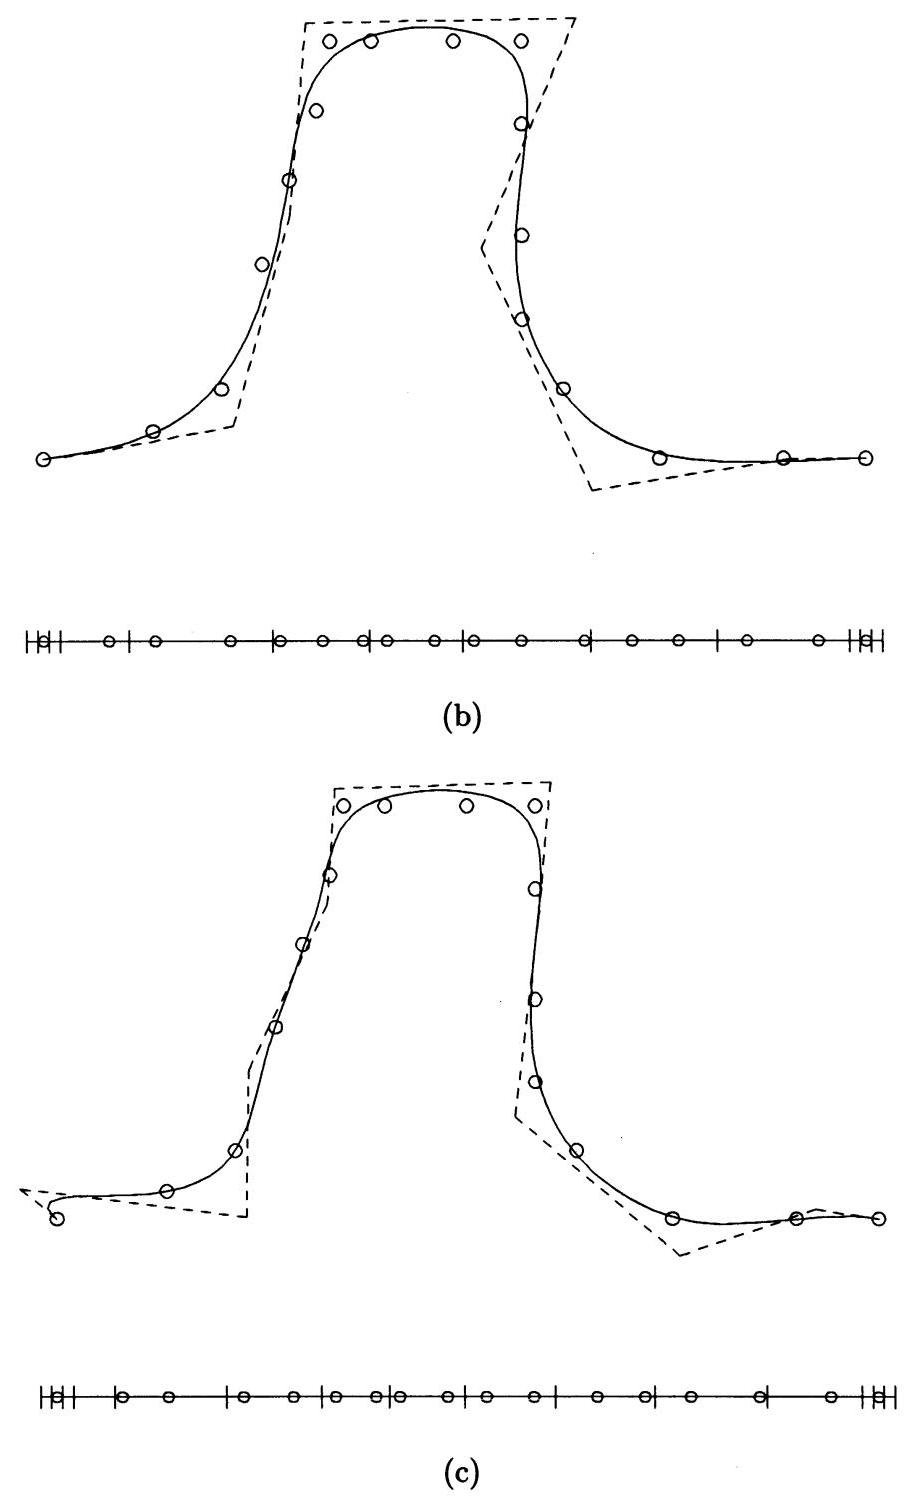
\includegraphics[max width=0.8\textwidth]{images/0193ba0d-ab19-7138-9798-cb281ce60de0_421_313_248_906_1505_0.jpg}
\end{center}
\hspace*{3em} 

图9.37。(续。)

现在设:

\({\mathbf{S}}_{k},k = 0,\ldots ,{m}_{u}\) ,是第 \(k\) 个不受约束的数据项(一个 \({\mathbf{Q}}^{u}\) 或一个 \({\mathbf{D}}^{u}\) );

\({\mathbf{T}}_{k},k = 0,\ldots ,{m}_{c}\) ,是第 \(k\) 个受约束的数据项(一个 \({\mathbf{Q}}^{c}\) 或一个 \({\mathbf{D}}^{c}\) );

\({w}_{k},k = 0,\ldots ,{m}_{u}\) ,是第 \(k\) 个权重(一个 \({w}^{q}\) 或一个 \({w}^{d}\) ).

定义向量/矩阵:

\(\mathbf{S} = \left\lbrack  {\mathbf{S}}_{k}\right\rbrack\) (一个包含 \({m}_{u} + 1\) 个元素的向量);

\(\mathbf{T} = \left\lbrack  {\mathbf{T}}_{k}\right\rbrack\) (一个包含 \({m}_{c} + 1\) 个元素的向量);

\(W = \left\lbrack  {w}_{k}\right\rbrack\) (一个 \(\left( {{m}_{u} + 1}\right)  \times  \left( {{m}_{u} + 1}\right)\) 对角矩阵，主对角线上为 \({w}_{k}\) );

\(\mathbf{P} = \left\lbrack  {\mathbf{P}}_{k}\right\rbrack\) (包含 \(n + 1\) 个未知控制点的向量);

\(N = \left\lbrack  {N{D}_{i,p}\left( {\bar{u}}_{k}\right) }\right\rbrack\) ,其中 \(N{D}_{i,p}\left( {\bar{u}}_{k}\right)\) 是第 \(i\) 个基函数或其一阶导数，在 \({\bar{u}}_{k}\) 处求值，这是一个与不受约束数据项对应的参数值；这是一个 \(\left( {{m}_{u} + 1}\right)  \times  \left( {n + 1}\right)\) 标量矩阵;

\(M = \left\lbrack  {M{D}_{i,p}\left( {\bar{u}}_{k}\right) }\right\rbrack\) ,其中 \(M{D}_{i,p}\left( {\bar{u}}_{k}\right)\) 是第 \(i\) 个基函数或其一阶导数，在 \({\bar{u}}_{k}\) 处求值，这是一个与受约束数据项对应的参数值；这是一个 \(\left( {{m}_{c} + 1}\right)  \times  \left( {n + 1}\right)\) 标量矩阵.

\({\bar{u}}_{k}\) 可以使用公式 (9.5) 计算，节点 \({u}_{j}\) 根据公式 (9.68) 和公式 (9.69) 计算(在公式 [9.68] 中将 \(m\) 替换为 \(r\) ).

确定曲线基本上是一个约束最小化问题，涉及 \(n + 1\) 个未知数( \({\mathbf{P}}_{i}\) )和 \({m}_{c} + 1\) 个约束。标准的解决方法是使用拉格朗日乘数(见 [Kapl52])。其思想是引入 \({m}_{c} + 1\) 个额外的未知数 \({\lambda }_{k}\) (拉格朗日乘数)，从而获得一个分区 \(\left( {n + {m}_{c} + 2}\right)  \times  \left( {n + {m}_{c} + 2}\right)\) 方程组。从这个方程组中，首先为 \({m}_{c} + 1{\lambda }_{k}\) 得到一个解，随后为 \(n + 1{\mathbf{P}}_{i}\) 得到解。设

\[
\mathbf{A} = \left\lbrack  {\lambda }_{k}\right\rbrack
\]

为拉格朗日乘数的向量；注意每个 \({\lambda }_{k}\) 是一个与 \(\left\{  {\mathbf{Q}}_{i}\right\}\) 和 \(\left\{  {\mathbf{D}}_{i\left( j\right) }\right\}\) 具有相同维度的向量。

无约束方程为

\[
N\mathbf{P} = \mathbf{S}
\]

而约束方程为

\[
M\mathbf{P} = \mathbf{T}
\]

无约束方程中的误差为 \(\mathbf{S} - N\mathbf{P}\) ，我们希望在 \(M\mathbf{P} = \mathbf{T}\) 的约束下最小化该误差的加权平方和。因此，使用拉格朗日乘数，我们希望最小化表达式

\[
\left( {{\mathbf{S}}^{T} - {\mathbf{P}}^{T}{N}^{T}}\right) W\left( {\mathbf{S} - N\mathbf{P}}\right)  + {\mathbf{A}}^{T}\left( {M\mathbf{P} - \mathbf{T}}\right)
\]

关于未知数 \(\mathbf{A}\) 和 \(\mathbf{P}\) 。对其进行微分并设其等于零，得到

\[
- 2\left( {{\mathbf{S}}^{T}{WN} - {\mathbf{P}}^{T}{N}^{T}{WN}}\right)  + {\mathbf{A}}^{T}M = 0
\]

\[
M\mathbf{P} - \mathbf{T} = 0
\]

转置并从 \(\mathbf{A}\) 中提取 2，得到

\[
{N}^{T}{WN}\mathbf{P} + {M}^{T}\mathbf{A} = {N}^{T}W\mathbf{S} \tag{9.71}
\]

\[
M\mathbf{P} = \mathbf{T} \tag{9.72}
\]

或以分区矩阵形式表示

\[
\left\lbrack  \begin{matrix} {N}^{T}{WN} & {M}^{T} \\  M & 0 \end{matrix}\right\rbrack  \left\lbrack  \begin{array}{l} \mathbf{P} \\  \mathbf{A} \end{array}\right\rbrack   = \left\lbrack  \begin{matrix} {N}^{T}W\mathbf{S} \\  \mathbf{T} \end{matrix}\right\rbrack   \tag{9.73}
\]

我们必须解方程 (9.73) 以求得 \(\mathbf{A}\) 和 \(\mathbf{P}\) 。如果 \({N}^{T}{WN}\) 和 \(M{\left( {N}^{T}WN\right) }^{-1}{M}^{T}\) 都是可逆的，则存在唯一解。这可以通过解方程 (9.71) 来看出，得到 \(\mathbf{P}\) ，即

\[
\mathbf{P} = {\left( {N}^{T}WN\right) }^{-1}{N}^{T}W\mathbf{S} - {\left( {N}^{T}WN\right) }^{-1}{M}^{T}\mathbf{A} \tag{9.74}
\]

乘以 \(M\) 得到

\[
M\mathbf{P} = M{\left( {N}^{T}WN\right) }^{-1}{N}^{T}W\mathbf{S} - M{\left( {N}^{T}WN\right) }^{-1}{M}^{T}\mathbf{A}
\]

最后，从方程 (9.72) 中我们发现

\[
M{\left( {N}^{T}WN\right) }^{-1}{M}^{T}\mathbf{A} = M{\left( {N}^{T}WN\right) }^{-1}{N}^{T}W\mathbf{S} - \mathbf{T} \tag{9.75}
\]

或

\[
\mathbf{A} = {\left( M{\left( {N}^{T}WN\right) }^{-1}{M}^{T}\right) }^{-1}\left( {M{\left( {N}^{T}WN\right) }^{-1}{N}^{T}W\mathbf{S} - \mathbf{T}}\right)  \tag{9.76}
\]

因此，我们首先求解 \(\mathbf{A}\) ，然后通过将 \(\mathbf{A}\) 代入方程 (9.74) 来求解 \(\mathbf{P}\) 。

算法 A9.6 实现了加权和约束最小二乘曲线拟合。输入为:

\(\mathrm{Q}\left\lbrack  {\mathrm{r} + 1}\right\rbrack\) : 一个包含待拟合点的数组(包括约束和非约束点)；

r: \(Q\left\lbrack  \right\rbrack\) 的上标；

\(\mathrm{{Wq}}\left\lbrack  {\mathrm{r} + 1}\right\rbrack   : \mathrm{{Wq}}\left\lbrack  i\right\rbrack   > 0\) 表示 \({\mathbf{Q}}_{i}\) 是非约束的，而 \(\mathrm{{Wq}}\left\lbrack  i\right\rbrack\) 是权重 \({w}_{i}^{q};\mathrm{{Wq}}\left\lbrack  i\right\rbrack   < 0\) 表示 \({\mathbf{Q}}_{i}\) 是要约束的；

\(\mathrm{D}\left\lbrack  {\mathrm{s} + 1}\right\rbrack\) : 一个包含导数的数组； \(\mathrm{s} =  - 1\) 表示未指定导数；

s: 在 \(\mathrm{D}\left\lbrack  \right\rbrack\) 中有 \(s + 1\) 个导数；

I [s+1]: 一个整数数组；I [j] 给出与 \(D\left\lbrack  j\right\rbrack\) 中导数对应的点在 Q[] 中的索引(即 \(D\left\lbrack  j\right\rbrack   = {D}_{i\left( j\right) }\) )；

Wd \(\left\lbrack  {s + 1}\right\rbrack   :\) Wd \(\left\lbrack  j\right\rbrack   > 0\) 表示 \(D\left\lbrack  j\right\rbrack\) 是非约束的，而 Wd \(\left\lbrack  j\right\rbrack\) 是权重 \({w}_{i\left( j\right) }^{d};\texttt{Wd[j]} < 0\) 表示 \(\mathtt{D\left\lbrack  j\right\rbrack  }\) 是要约束的；

n: 一个具有 \(n + 1\) 个控制点的拟合；

p: 与度数 \(p\) 曲线的拟合。

输出节点 \(\mathrm{U}\) 和控制点 \(\mathrm{P}\) 。该算法使用 LU 分解(   )和前向后向(   )来反转矩阵 \(\left( {{N}^{T}{WN}}\right)\) 并求解拉格朗日乘子 A。由于算法构造 \(N\) 的方式， \(\left( {{N}^{T}{WN}}\right)\) 的半带宽小于 \(p + 1\) 。一般来说， \(\mathbf{A}\) 可以具有全带宽，但通常是一个小矩阵。使用第 2 章中的适当算法来确定节点跨度并计算基函数及其导数。以下局部数组是必需的:

ub \(\left\lbrack  {r + 1}\right\rbrack\) : 参数；

N[mu+1][n+1], M[mc+1][n+1], S[mu+1], T[mc+1], A[mc+1]: 与之前定义的矩阵对应的数组(除了 S[]，它是 \(W\mathbf{S}\) )；

\(\mathrm{W}\left\lbrack  {\mathrm{{mu}} + 1}\right\rbrack\) : 权重；由于矩阵 \(W\) 是对角的，仅需要长度为 \({m}_{u} + 1\) 的向量；

funs [2] [p+1]: 包含基函数及其指定的导数(见算法 A2.2 和 A2.3)。

此外，还需要几个局部数组用于临时存储在方程 (9.71)-(9.76) 中计算的矩阵。

\HRule

ALGORITHM A9.6

\hspace*{2em} WCLeastSquaresCurve(Q, r, Wq, D, s, I, Wd, n, p, U, P)

\hspace*{5em} \{ /* Weighted \& constrained least squares curve fit */

\hspace*{8em} /* Input: Q, r, Wq, D, s, I, Wd, n, p */

\hspace*{8em} /* Output: U, P */

\hspace*{5em} ru = -1; rc = -1;

\hspace*{5em} for (i=0; i<=r; i++)

\hspace*{7em} if (Wq[i] > 0.0) ru = ru+1 ;

\hspace*{9em} else \(\;\mathrm{{rc}} = \mathrm{{rc}} + 1\) ;

\hspace*{5em} su = -1; sc = -1;

\hspace*{5em} for (j=0; j<=s; j++)

\hspace*{7em} if (Wd[j] > 0.0) su = su+1 ;

\hspace*{9em} else sc = sc+1;

\hspace*{5em} \(\mathrm{{mu}} = \mathrm{{ru}} + \mathrm{{su}} + 1;\;\mathrm{{mc}} = \mathrm{{rc}} + \mathrm{{sc}} + 1\) ;

\hspace*{5em} if (mc >= n || mc+n >= mu+1) return(error);

\hspace*{5em} Compute and load parameters \({\bar{u}}_{k}\) into ub[] (Eq.[9.5]);

\hspace*{5em} Compute and load the knots into U[] (Eqs.[9.68],[9.69]);

\hspace*{12em} /* Now set up arrays \(N,W,\mathbf{S},\mathbf{T},M *\) /

\hspace*{5em} j = 0; /* current index into I[] */

\hspace*{5em} mu2 = 0; mc2 = 0; /* counters up to mu and mc */

\hspace*{5em} for (i = 0; i<=r; i++)

\hspace*{7em} \{

\hspace*{7em} span = FindSpan(n, p, ub[i], U);

\hspace*{7em} dflag = 0 ;

\hspace*{7em} if (j <= s)

\hspace*{9em} if (i == I[j]) dflag = 1 ;

\hspace*{2em} if \(\left( {\text{ dflag } =  = 0}\right) \;\) BasisFuns \(\left( {\text{ span },{ub}\left\lbrack  i\right\rbrack  ,p,U,\text{ funs }}\right)\) ;

\hspace*{3em} else DersBasisFuns(span, ub[i], p,1, U, funs);

\hspace*{2em} if (Wq[i] > 0.0 )

\hspace*{3em} \{ /* Unconstrained point */

\hspace*{3em} W[mu2] = Wq[i];

\hspace*{3em} Load the mu2th row of N[][] from funs[0][];

\hspace*{3em} S[mu2] = W[mu2]*Q[i];

\hspace*{3em} mu2 = mu2+1;

\hspace*{3em} \}

\hspace*{3em} else

\hspace*{3em} \{ /* Constrained point */

\hspace*{3em} Load the mc2th row of M[][] from funs[0][];

\hspace*{3em} T[mc2] = Q[i];

\hspace*{3em} mc2 = mc2+1;

\hspace*{3em} \}

\hspace*{2em} if (dflag == 1)

\hspace*{3em} \{ /* Derivative at this point */

\hspace*{3em} if (Wd[j] > 0.0 )

\hspace*{4em} \{ /* Unconstrained derivative */

\hspace*{4em} W[mu2] = Wd[j];

\hspace*{4em} Load the mu2th row of N[][] from funs[1][];

\hspace*{4em} \(S\left\lbrack  {mu2}\right\rbrack   = W\left\lbrack  {mu2}\right\rbrack   * D\left\lbrack  j\right\rbrack  ;\)

\hspace*{4em} mu2 = mu2+1;

\hspace*{4em} \}

\hspace*{4em} else

\hspace*{4em} \{ /* Constrained derivative */

\hspace*{4em} Load the mc2th row of M[][] from funs[1][];

\hspace*{4em} T[mc2] = D[j];

\hspace*{4em} mc2 = mc2+1;

\hspace*{4em} \}

\hspace*{3em} j = j+1;

\hspace*{3em} \}

\hspace*{1em} \} /* End of for-loop i=0,..., r */

Compute the matrices \({N}^{T}{WN}\) and \({N}^{T}W\mathbf{S}\) ;

LUDecomposition \(\left( {{N}^{T}{WN},\mathrm{n} + 1,\mathrm{p}}\right)\) ;

if (mc < 0 )

\hspace*{1em} \{ /* No constraints */

\hspace*{1em} Use ForwardBackward(   ) to solve for the control points \(P\left\lbrack  \right\rbrack\) .

\hspace*{4em} Eq. (9.71) reduces to \(\left( {{N}^{T}{WN}}\right) \mathbf{P} = {N}^{T}W\mathbf{S}\) .

\hspace*{1em} return;

\hspace*{1em} \}

Compute the inverse \({\left( {N}^{T}WN\right) }^{-1}\) , using ForwardBackward(   ).

Do matrix operations to get: \(M{\left( {N}^{T}WN\right) }^{-1}{M}^{T}\) and

\hspace*{3em} \(M{\left( {N}^{T}WN\right) }^{-1}\left( {{N}^{T}W\mathbf{S}}\right)  - \mathbf{T};\)

Solve Eq.(9.75) for the Lagrange multipliers, load into A[];

\HRule

然后 \(\mathbf{P} = {\left( {N}^{T}WN\right) }^{-1}\left( {\left( {{N}^{T}W\mathbf{S}}\right)  - {M}^{T}\mathbf{A}}\right)\) ，方程 (9.74)；

\}

图 9.38-9.43 显示了加权和约束曲线拟合的几个示例。图 9.38 显示了一个无约束的拟合，所有权重均设置为 1。在图 9.39 中，权重 \({w}_{4}^{q},{w}_{5}^{q},{w}_{6}^{q}\) 和 \({w}_{7}^{q}\) 各增加到 100，从而导致曲线向数据点 \({\mathbf{Q}}_{4},\ldots ,{\mathbf{Q}}_{7}\) 拉动。请注意，尽管图形具有误导性，但曲线并未通过端点。图 9.40 显示了一个约束拟合，其中点(用方块标记)以及导数(箭头向量)作为约束。曲线通过方块标记的点，并在这些点上与指定的向量相切。在图 9.41 中引入了两个额外的权重 \({w}_{5}^{q} = {100}\) 和 \({w}_{15}^{q} = {100}\) 。图 9.42 显示了与图 9.40 相同的曲线，只是使用了两个新的内部导数。类似地，图 9.43 与图 9.42 相同，只是添加了权重 \({w}_{4}^{q} = {50}\) 和 \({w}_{16}^{q} = {20}\) 。



\subsection{最小二乘曲面逼近}

现在我们转向具有固定数量控制点的曲面逼近。设 \(\left\{  {\mathbf{Q}}_{k,\ell }\right\}  ,k = 0,\ldots ,r\) 和 \(\ell  = 0,\ldots ,s\) 为要被逼近的 \(\left( {r + 1}\right)  \times  \left( {s + 1}\right)\) 点集，采用 a(p, q) 次非理性曲面，具有 \(\left( {n + 1}\right)  \times  \left( {m + 1}\right)\) 个控制点。尽管可以建立并解决一般的最小二乘曲面拟合问题，无论是线性还是非线性，且有无权重和约束，但这项任务比曲线的情况复杂得多。我们在这里提出了一种曲面逼近方案，该方案基于我们的最小二乘曲线方案。

\begin{center}
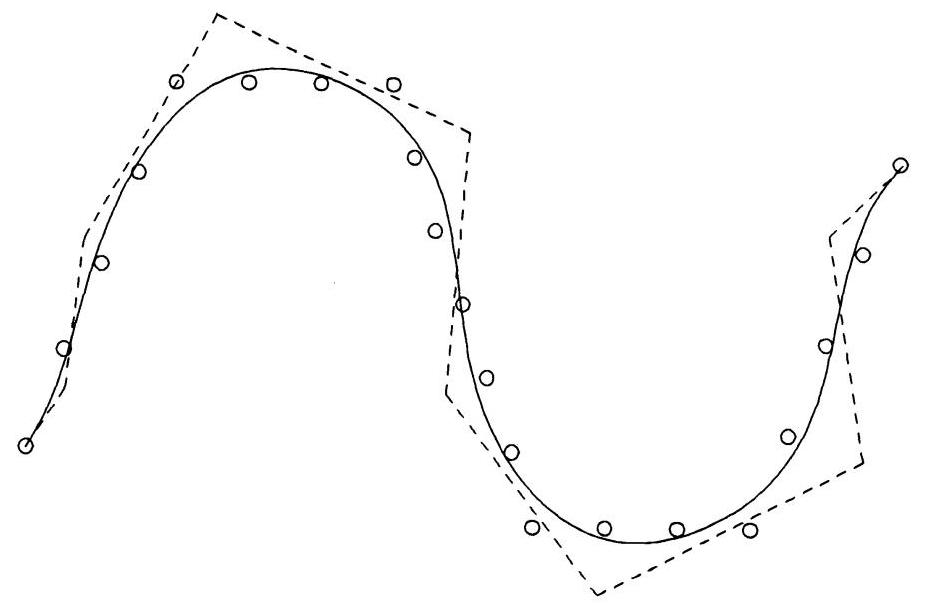
\includegraphics[max width=0.8\textwidth]{images/0193ba0d-ab19-7138-9798-cb281ce60de0_426_297_1414_926_606_0.jpg}
\end{center}
\hspace*{3em} 

图 9.38。所有权重均等于一的无约束拟合；注意曲线并未通过端点。

420 曲线和曲面拟合

\begin{center}
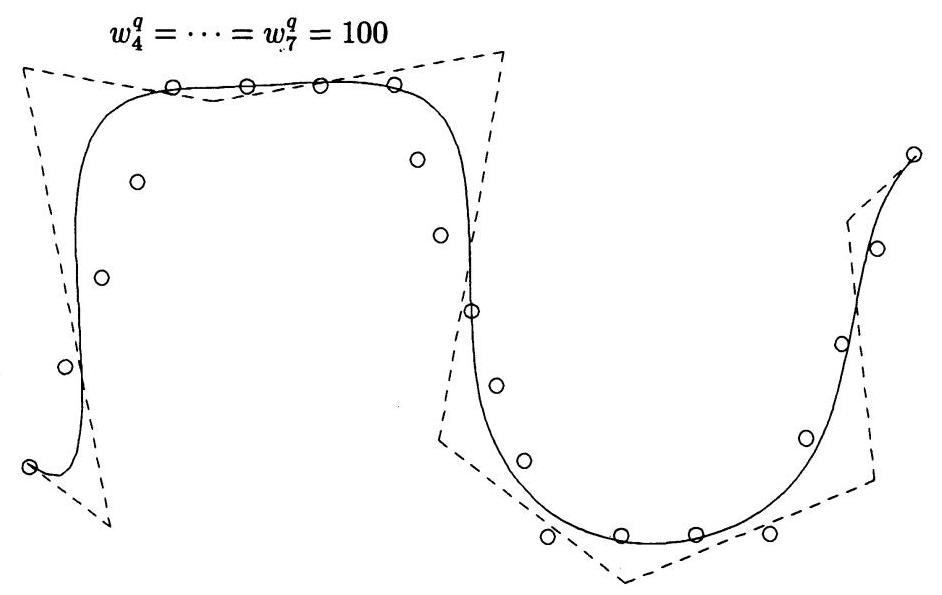
\includegraphics[max width=0.8\textwidth]{images/0193ba0d-ab19-7138-9798-cb281ce60de0_427_294_262_942_595_0.jpg}
\end{center}
\hspace*{3em} 

图 9.39. 不受约束的加权拟合 \({w}_{4}^{q} = {w}_{5}^{q} = {w}_{6}^{q} = {w}_{7}^{q} = {100}\) ；曲线不通过端点。

非常简单，并且对于大多数应用来说相当足够。与全局表面插值相同，我们只需在一个方向上拟合数据中的曲线，然后在另一个方向上通过得到的控制点拟合曲线。

\begin{center}
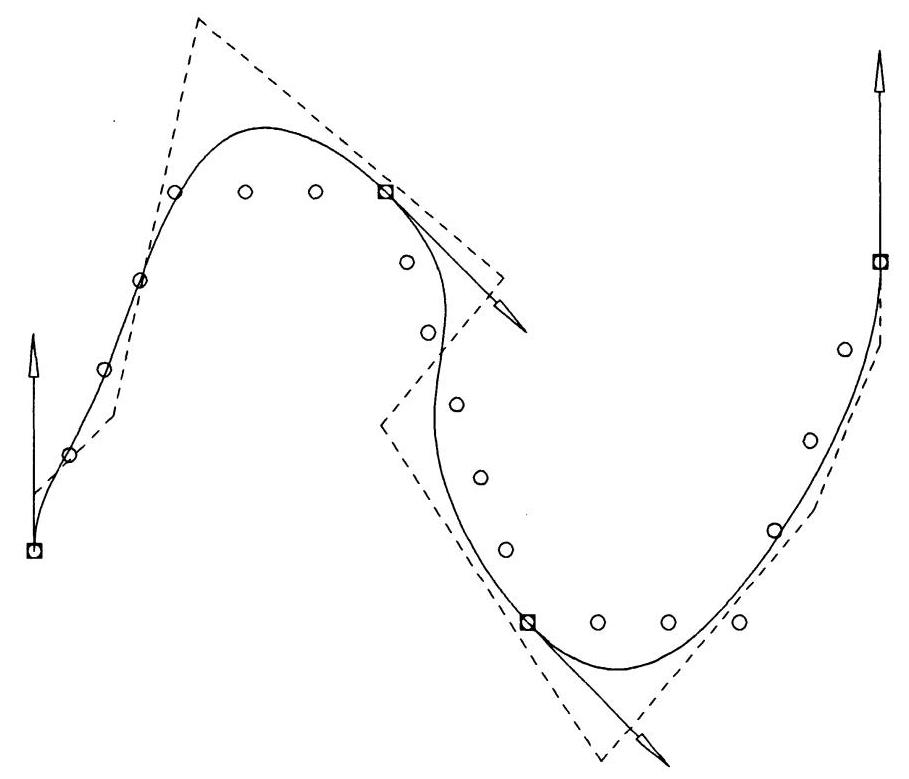
\includegraphics[max width=0.8\textwidth]{images/0193ba0d-ab19-7138-9798-cb281ce60de0_427_306_1268_909_779_0.jpg}
\end{center}
\hspace*{3em} 

图 9.40. 受约束的曲线拟合；点约束用方框标记，切线约束用箭头表示，所有权重均为一。

\begin{center}
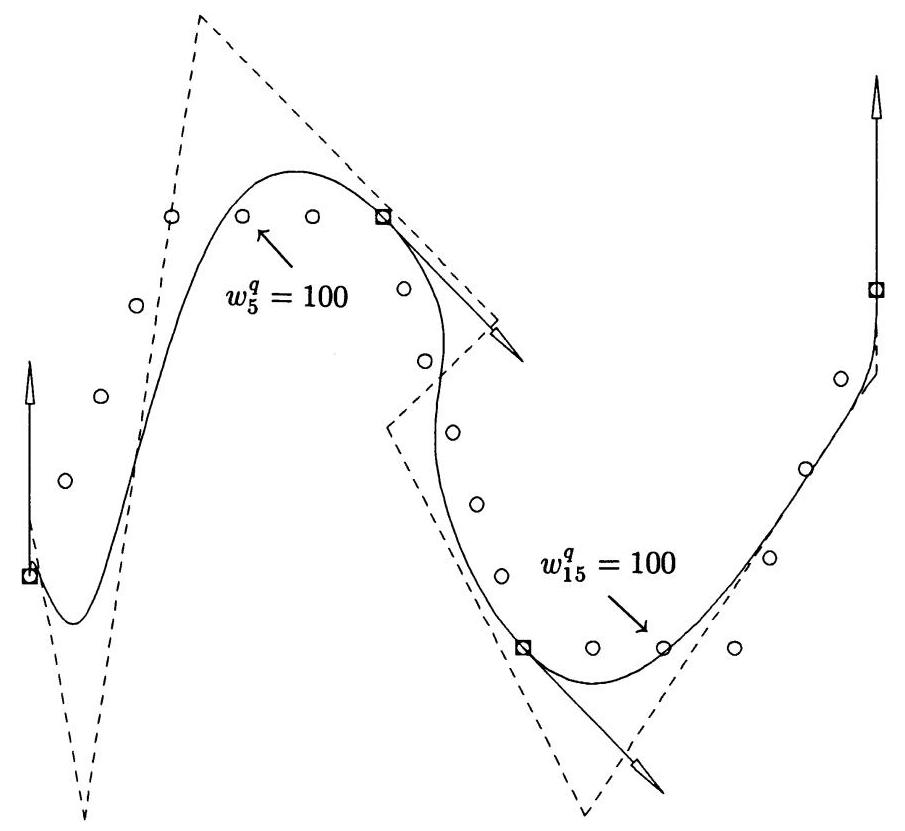
\includegraphics[max width=0.8\textwidth]{images/0193ba0d-ab19-7138-9798-cb281ce60de0_428_315_252_905_831_0.jpg}
\end{center}
\hspace*{3em} 

图 9.41. 来自图 9.40 的曲线，权重为 \({w}_{5}^{q} = {w}_{15}^{q} = {100}\) 。

算法 A9.7 精确插值角点 \({\mathbf{Q}}_{0,0},{\mathbf{Q}}_{r,0},{\mathbf{Q}}_{0,s}\) 和 \({\mathbf{Q}}_{r,s}\) ，并近似剩余的 \(\left\{  {\mathbf{Q}}_{k,l}\right\}\) 。它使用由方程 (9.63) 和 (9.65)-(9.67) 给出的重复最小二乘曲线拟合。它拟合 \(s + 1\) 行数据。

\begin{center}
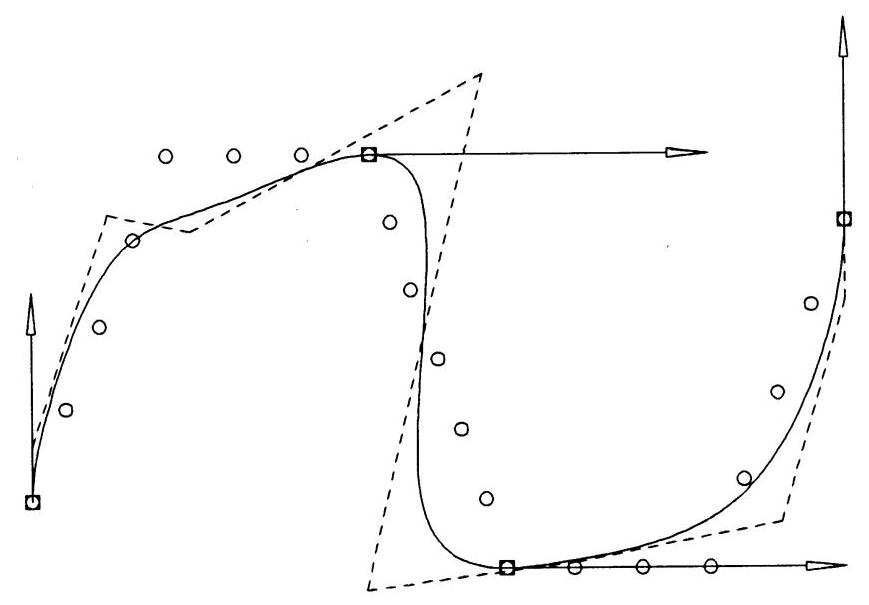
\includegraphics[max width=0.7\textwidth]{images/0193ba0d-ab19-7138-9798-cb281ce60de0_428_329_1460_869_605_0.jpg}
\end{center}
\hspace*{3em} 

图 9.42. 来自图 9.40 的曲线，但使用两个新的切线约束。

\begin{center}
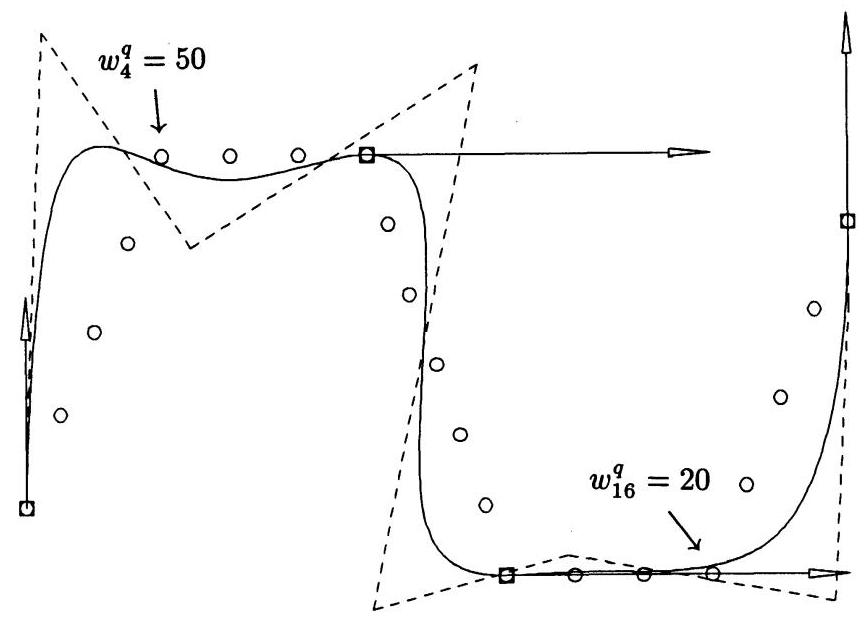
\includegraphics[max width=0.7\textwidth]{images/0193ba0d-ab19-7138-9798-cb281ce60de0_429_334_268_868_624_0.jpg}
\end{center}
\hspace*{3em} 

图 9.43. 来自图 9.42 的曲线，但权重为 \({w}_{4}^{q} = {50}\) 和 \({w}_{16}^{q} = {20}\) 。

首先，将得到的控制点存储在局部数组 Temp[n+1][s+1] 中。然后，它在这些控制点上拟合，以生成 \(\left( {n + 1}\right)  \times  \left( {m + 1}\right)\) 表面控制点。注意，矩阵 \(N\) 和 \({N}^{T}N\) 只需在每个方向上计算一次，而 \({N}^{T}N\) 的 LU 分解也只需在每个方向上进行一次。我们需要局部数组 Nu[r-1][n-1] 和 NTNu[n-1][n-1] 用于 \(u\) 方向的拟合，以及 \(\mathrm{{Nv}}\left\lbrack  {\mathrm{s} - 1}\right\rbrack  \left\lbrack  {\mathrm{m} - 1}\right\rbrack\) 和 \(\mathrm{{NTNv}}\left\lbrack  {\mathrm{m} - 1}\right\rbrack  \left\lbrack  {\mathrm{m} - 1}\right\rbrack\) 用于 \(v\) 方向的拟合。方程 (9.68) 的向量 \(\mathbf{R}\) 存储在 Ru[n-1] 和 Rv[m-1] 中。

\HRule

ALGORITHM A9.7

\hspace*{1em} GlobalSurfApproxFixednm(r, s, Q, p, q, n, m, U, V, P)

\hspace*{3em} \{ /* Global surface approx with fixed num of ctrl pts */

\hspace*{5em} /* Input: r, s, Q, p, q, n, m */

\hspace*{5em} /* Output: U, V, P */

\hspace*{3em} SurfMeshParams(r, s, Q, ub, vb);

\hspace*{3em} Compute knots U by Eqs. (9.68), (9.69);

\hspace*{3em} Compute knots V by Eqs. (9.68), (9.69);

\hspace*{3em} Compute Nu[][] and NTNu[][] using Eq.(9.66);

\hspace*{3em} LUDecomposition(NTNu, n-1, p);

\hspace*{3em} for (j=0; j<=s; j++)

\hspace*{4em} \{ /* u direction fits */

\hspace*{4em} \(\operatorname{Temp}\left\lbrack  0\right\rbrack  \left\lbrack  j\right\rbrack   = {\mathbf{Q}}_{0,j};\;\operatorname{Temp}\left\lbrack  n\right\rbrack  \left\lbrack  j\right\rbrack   = {\mathbf{Q}}_{r,j};\)

\hspace*{4em} Compute and load Ru[] (Eqs.[9.63],[9.67]);

\hspace*{4em} Call ForwardBackward(   ) to get the control points

\hspace*{7em} Temp[1][j],..., Temp[n-1][j];

\hspace*{4em} \}

\hspace*{3em} Compute Nv[][] and NTNv[][] using Eq.(9.66);

\hspace*{3em} LUDecomposition(NTNv, m-1, q);

for (i = 0 ; i<=n ; i++)

\hspace*{1em} \{ /* v direction fits */

\hspace*{1em} \(P\left\lbrack  i\right\rbrack  \left\lbrack  0\right\rbrack   = \operatorname{Temp}\left\lbrack  i\right\rbrack  \left\lbrack  0\right\rbrack  ;\;P\left\lbrack  i\right\rbrack  \left\lbrack  m\right\rbrack   = \operatorname{Temp}\left\lbrack  i\right\rbrack  \left\lbrack  s\right\rbrack  ;\)

\hspace*{1em} Compute and load Rv[] (Eqs.[9.63],[9.67]);

\hspace*{1em} Call ForwardBackward(   ) to get the control points

\hspace*{4em} \(P\left\lbrack  i\right\rbrack  \left\lbrack  1\right\rbrack  ,\ldots ,P\left\lbrack  i\right\rbrack  \left\lbrack  {m - 1}\right\rbrack\) ;

\hspace*{1em} \}

\}

\HRule

图 9.44-9.47 说明了表面拟合。图 9.44 显示了通过直线连接的原始数据。图 9.45a 描绘了使用 \(\left( {5 \times  6}\right)\) 控制网的度数(2,3)最小二乘表面拟合。近似误差显示在图 9.45b 中。图 9.46a 显示了使用 \(\left( {8 \times  8}\right)\) 网的近似。其近似质量要好得多，如图 9.46b 所示。为了比较，图 9.47 显示了对图 9.44 中数据的度数(2,3)全局插值(使用弦长参数)。

当然，可以先拟合 \(r + 1\) 列，然后再拟合结果 \(m + 1\) 控制点的行。一般来说，结果并不相同。我们不知道有什么标准可以提前决定哪种方法会为特定数据集提供“最佳”拟合。显然，这种技术可以很容易地扩展以适应边界上的点和导数约束以及加权。内部约束则更为复杂。假设 \({\mathbf{Q}}_{{k}_{0},{\ell }_{0}},0 < {k}_{0} < r\) 和 \(0 <\)  \({\ell }_{0} < s\) 需要被约束。该点在 \(u\) 方向上受到约束。

\begin{center}
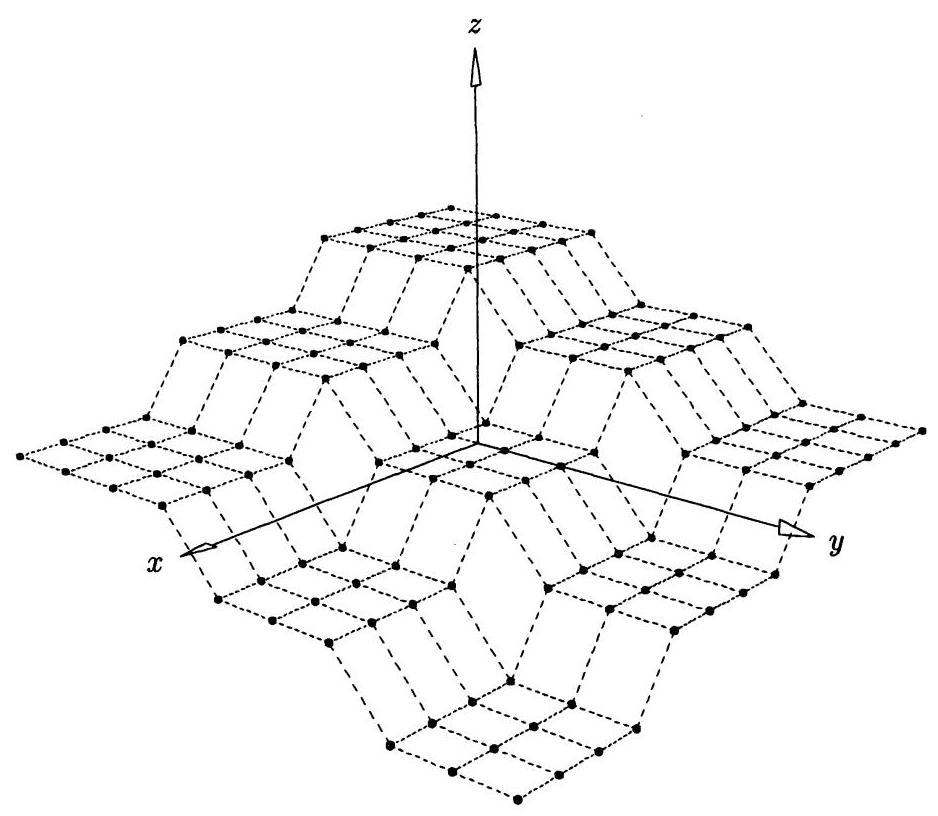
\includegraphics[max width=0.8\textwidth]{images/0193ba0d-ab19-7138-9798-cb281ce60de0_430_292_1269_938_816_0.jpg}
\end{center}
\hspace*{3em} 

图 9.44. 表面近似的数据集。

\begin{center}
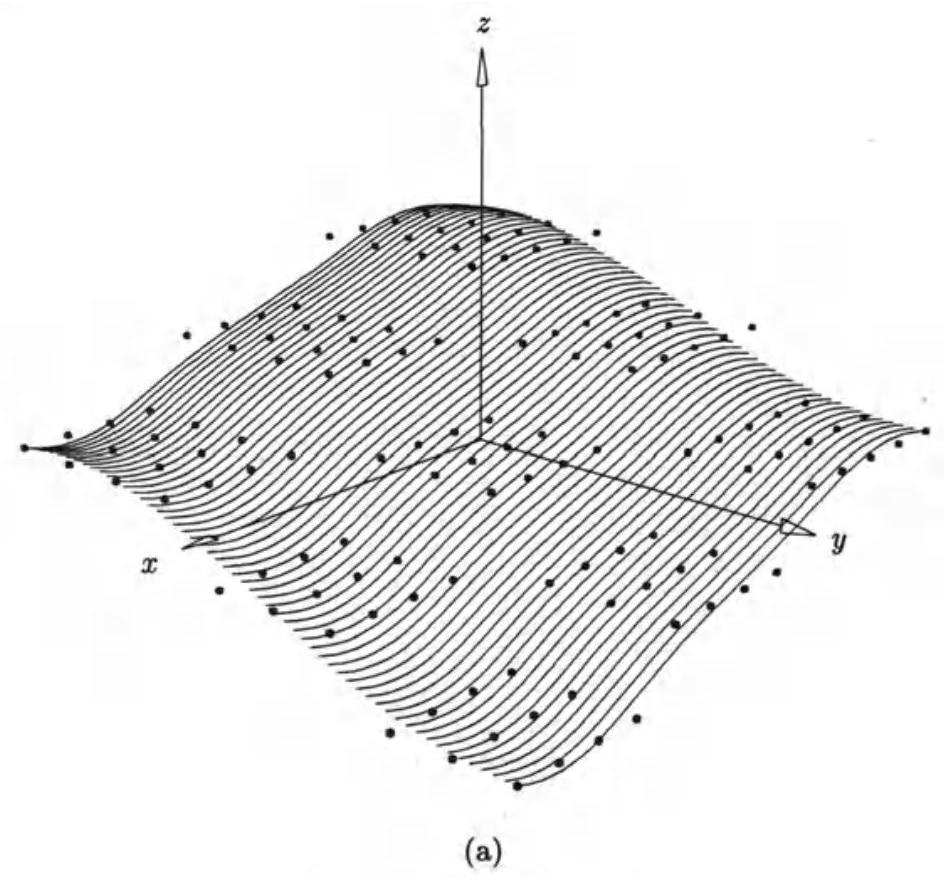
\includegraphics[max width=0.8\textwidth]{images/0193ba0d-ab19-7138-9798-cb281ce60de0_431_304_253_944_877_0.jpg}
\end{center}
\hspace*{3em} 

图 9.45. 使用 \(\left( {5 \times  6}\right)\) 控制网的度数(2,3)表面的最小二乘拟合。(a) 表面近似；(b) 误差表面(在数据点处测量的误差)。

曲线拟合，如算法 A9.6 所示。然后，如果 \({\bar{u}}_{{k}_{0}} \in  \left\lbrack  {{u}_{i},{u}_{i + 1}}\right)\) ，则点 \(\operatorname{Temp}\lbrack i -\)  \(p\rbrack \left\lbrack  {\ell }_{0}\right\rbrack  ,\ldots ,\operatorname{Temp}\left\lbrack  i\right\rbrack  \left\lbrack  {\ell }_{0}\right\rbrack\) 必须在 \(v\) 方向上受到约束。


\subsection{在指定精度内的逼近}

我们现在回到将数据近似到某个用户指定的误差范围内的问题， \(E\) 。正如本节开始所述，迭代方法要么从少量控制点开始，拟合、检查偏差，并在必要时添加控制点(类型1)；要么从大量控制点开始，拟合、检查偏差，并在可能的情况下丢弃控制点(类型2)。前面提到的基于最小二乘法的方法适用于拟合步骤。偏差检查步骤通常测量最大距离，既可以表示为

\[
\mathop{\max }\limits_{{0 \leq  k \leq  m}}\left| {{\mathbf{Q}}_{k} - \mathbf{C}\left( {\bar{u}}_{k}\right) }\right| \text{ or }\mathop{\max }\limits_{\substack{{0 \leq  k \leq  r} \\  {0 \leq  \ell  \leq  s} }}\left| {{\mathbf{Q}}_{k,\ell } - \mathbf{S}\left( {{\bar{u}}_{k},{\bar{v}}_{\ell }}\right) }\right|  \tag{9.77}
\]

或表示为

\[
\mathop{\max }\limits_{{0 \leq  k \leq  m}}\left( {\mathop{\min }\limits_{{0 \leq  u \leq  1}}\left| {{\mathbf{Q}}_{k} - \mathbf{C}\left( u\right) }\right| }\right) \;\text{ or }\;\mathop{\max }\limits_{\substack{{0 \leq  k \leq  r} \\  {0 \leq  \ell  \leq  s} }}\left( {\mathop{\min }\limits_{\substack{{0 \leq  u \leq  1} \\  {0 \leq  v \leq  1} }}\left| {{\mathbf{Q}}_{k,\ell } - \mathbf{S}\left( {u,v}\right) }\right| }\right)  \tag{9.78}
\]

426 曲线和曲面拟合 我们将方程(9.78)称为最大范数偏差。它使用方程(6.4)-(6.9)来计算每个 \({\mathbf{Q}}_{k}\left( {\mathbf{Q}}_{k,\ell }\right)\) 到 \(\mathbf{C}\left( u\right) \left( {\mathbf{S}\left( {u,v}\right) }\right)\) 的最小距离。 \({\bar{u}}_{k}\left( {{\bar{u}}_{k},{\bar{v}}_{\ell }}\right)\) 作为牛顿迭代的良好起始点。显然，应用方程(9.78)的成本高于方程(9.77)。然而，这通常是用户希望测量的内容，并且通常会导致具有更少控制点的曲线和曲面，因为

\[
\mathop{\min }\limits_{{0 \leq  u \leq  1}}\left| {{\mathbf{Q}}_{k} - \mathbf{C}\left( u\right) }\right|  \leq  \left| {{\mathbf{Q}}_{k} - \mathbf{C}\left( {\bar{u}}_{k}\right) }\right|  \tag{9.79}
\]

\begin{center}
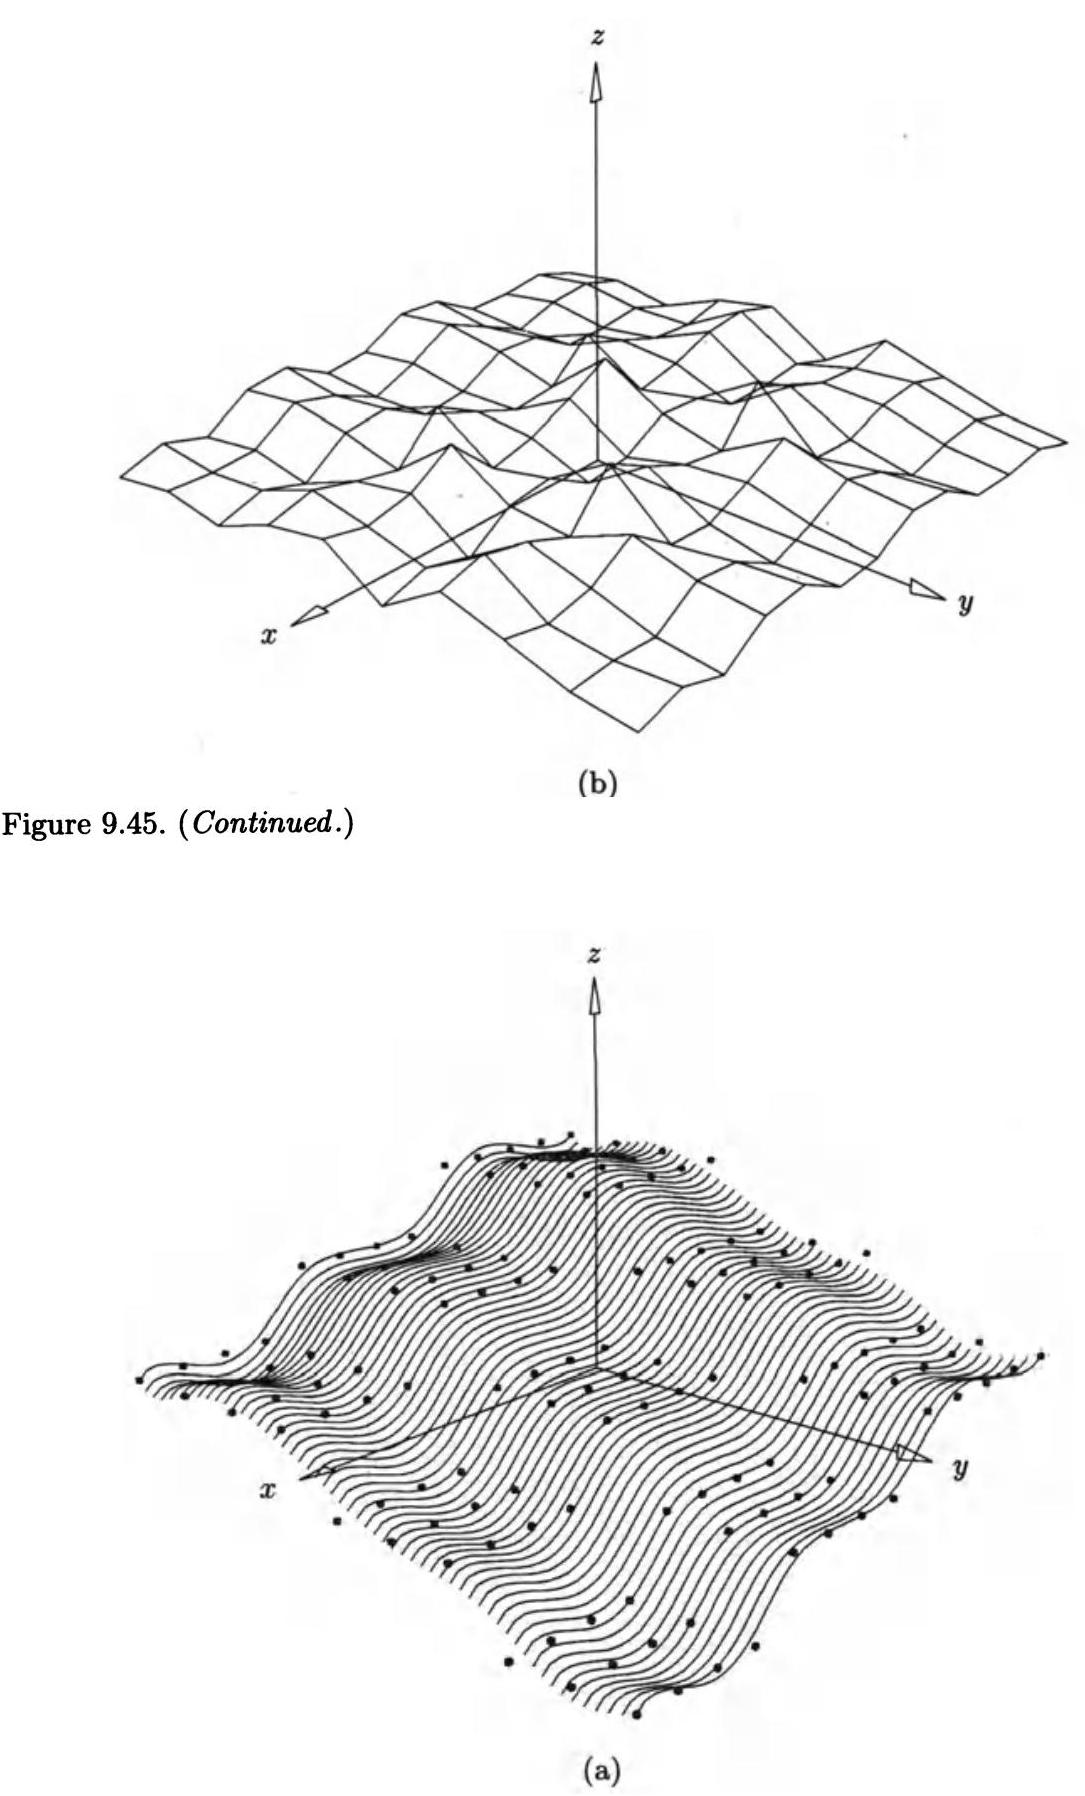
\includegraphics[max width=0.9\textwidth]{images/0193ba0d-ab19-7138-9798-cb281ce60de0_432_170_266_1085_1796_0.jpg}
\end{center}
\hspace*{3em} 

图9.46. 使用 \(\left( {8 \times  8}\right)\) 控制网的二次(2,3)曲面拟合的最小二乘曲面。 (a) 曲面近似；(b) 误差曲面(在数据点处测量的误差)。

\begin{center}
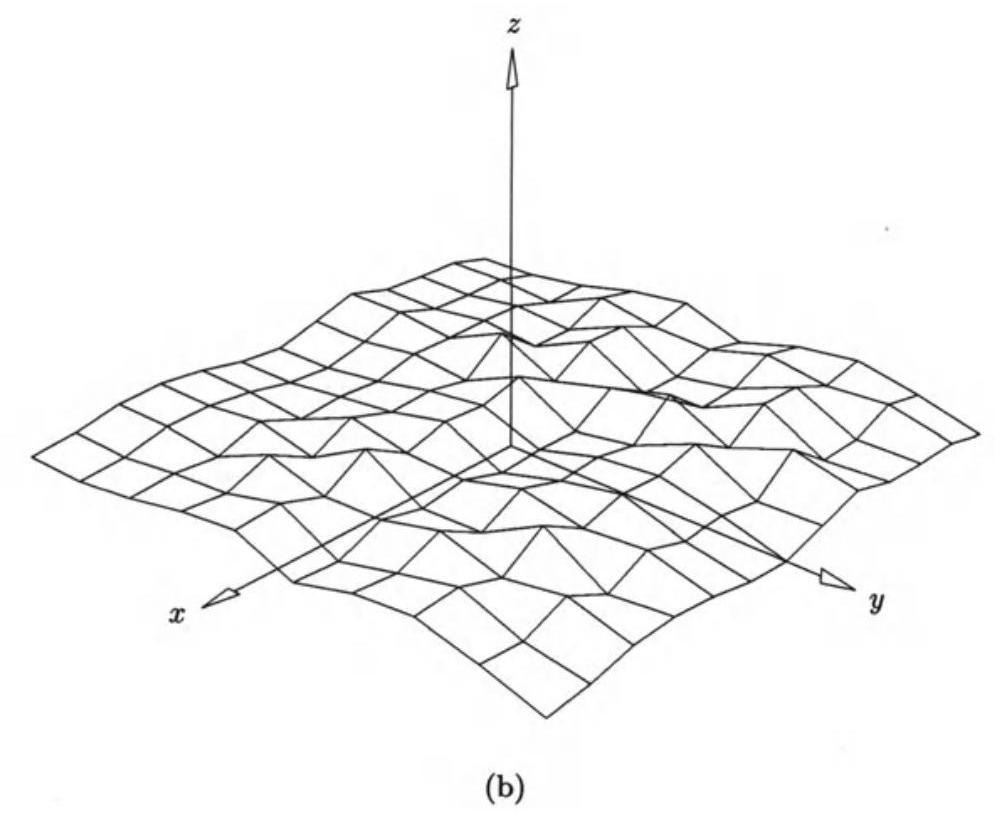
\includegraphics[max width=0.9\textwidth]{images/0193ba0d-ab19-7138-9798-cb281ce60de0_433_344_266_995_813_0.jpg}
\end{center}
\hspace*{3em} 

图9.46. (续。)

\begin{center}
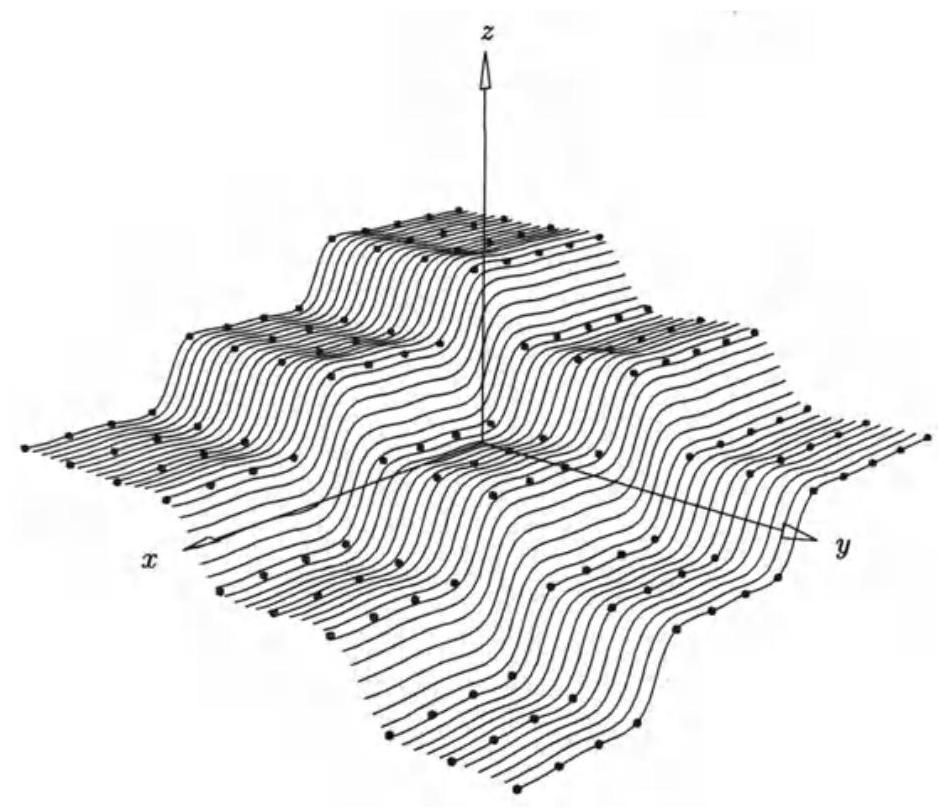
\includegraphics[max width=0.8\textwidth]{images/0193ba0d-ab19-7138-9798-cb281ce60de0_433_350_1254_949_808_0.jpg}
\end{center}
\hspace*{3em} 

图9.47. 显示在图9.44中的表面插值点。

我们强调，类型1和类型2的方法都可能无法收敛，这种情况必须在软件实现中处理。

一种类型 1 曲线逼近方法可以按如下方式进行。首先从 \(p + 1\) 控制点(最小值)开始。使用公式 (9.63) 和 (9.65) (9.67) 拟合曲线，或者如果需要内部约束，则使用算法 A9.6。在每次拟合后，使用公式 (9.78) 检查曲线偏差是否小于 \(E\) 。为每个节点区间维护记录，指示其是否已收敛；如果公式 (9.78) 对所有 \(k\) 满足 \({\bar{u}}_{k} \in  \left\lbrack  {{u}_{j},{u}_{j + 1}}\right)\) ，则区间 \(\left\lbrack  {{u}_{j},{u}_{j + 1}}\right)\) 已收敛。在每次拟合和随后的偏差检查后，在每个未收敛区间的中点添加一个节点，从而增加控制点。该算法必须处理在添加节点时区间可能变为空的情况(即，该区间不包含任何 \({\bar{u}}_{k}\) )，从而在拟合步骤中产生奇异的方程组。

一种类型 1 表面逼近方法可以以类似的方式实现，并提高效率。在偏差检查期间，确定具有最大偏差点数的行 \({\ell }_{0}\) 和列 \({k}_{0}\) ，这些偏差大于 \(E\) 。然后提取等参数曲线 \({\mathbf{C}}_{{\bar{u}}_{{k}_{0}}}\left( v\right)\) 和 \({\mathbf{C}}_{{\bar{v}}_{{\ell }_{0}}}\left( u\right)\) ，并独立地将它们逼近到 \(E\) 之内。这将产生新的(增加的)节点向量 \(U\) 和 \(V\) ，用于下一个表面拟合。使用这种方法，通常只需要进行几次表面拟合和随后的偏差检查。

我们现在开发一种类型 2 曲线近似方法，该方法结合了最小二乘拟合与第 5 章的节点移除技术。首先，我们需要更多的节点移除工具。设 \({u}_{r}\) 为一个 \(p\) 次非理性曲线的内部节点 \(\mathbf{C}\left( u\right) ,{u}_{r} \neq  {u}_{r + 1}\) ，并用 \(s\) 表示 \({u}_{r}\) 的重数，即对于 \(j = 1,\ldots ,s\) 有 \({u}_{r - s + j} = {u}_{r}\) 。设 \(\widehat{\mathbf{C}}\left( u\right)\) 为通过移除一个 \({u}_{r}\) 的出现而得到的曲线。回想一下，新控制点 \({\mathbf{P}}_{i}^{1}\) 和 \({\mathbf{P}}_{j}^{1}\) 分别通过公式 (5.28) 从左侧和右侧计算得出。移除后， \(\widehat{\mathbf{C}}\left( u\right)\) 与 \(\mathbf{C}\left( u\right)\) 不同；Tiller [Till92] 推导了两种情况的误差界限:

\begin{itemize}
\item 假设 \(\left( {p + s}\right) {\;\operatorname{mod}\;2} = 0\) ; 设定 \(k = \left( {p + s}\right) /2\) 和
\end{itemize}

\[
{B}_{r} = \left| {{\mathbf{P}}_{r - k} - {\alpha }_{r - k}{\mathbf{P}}_{r - k + 1}^{1} - \left( {1 - {\alpha }_{r - k}}\right) {\mathbf{P}}_{r - k - 1}^{1}}\right|  \tag{9.80}
\]

其中

\[
{\alpha }_{r - k} = \frac{{u}_{r} - {u}_{r - k}}{{u}_{r - k + p + 1} - {u}_{r - k}}
\]

\[
\text{ Then }\;\left| {\mathbf{C}\left( u\right)  - \widehat{\mathbf{C}}\left( u\right) }\right|  \leq  {N}_{r - k,p}\left( u\right) {B}_{r}\;\text{ for }u \in  \left\lbrack  {0,1}\right\rbrack   \tag{9.81}
\]

\begin{itemize}
\item 假设 \(\left( {p + s}\right) {\;\operatorname{mod}\;2} = 1\) ; 设定 \(k = \left( {p + s + 1}\right) /2\) 和
\end{itemize}

\[
{B}_{r} = \left| {{\mathbf{P}}_{r - k}^{1} - {\mathbf{P}}_{r - k + 1}^{1}}\right|  \tag{9.82}
\]

然后 \(\left| {\mathbf{C}\left( u\right)  - \widehat{\mathbf{C}}\left( u\right) }\right|  \leq  \left( {1 - {\alpha }_{r - k + 1}}\right) {N}_{r - k + 1,p}\left( u\right) {B}_{r}\)

\[
\text{ for }u \in  \left\lbrack  {0,1}\right\rbrack   \tag{9.83}
\]

与

\[
{\alpha }_{r - k + 1} = \frac{{u}_{r} - {u}_{r - k + 1}}{{u}_{r - k + p + 2} - {u}_{r - k + 1}}
\]

\({B}_{r}\) 只是节点移除算法 A5.8 中计算的距离。算法 A9.8 是算法 A5.8 的修改版，仅计算 \({B}_{r}\) 。

\HRule

\section*{ALGORITHM A9.8}

GetRemovalBndCurve(n, p, U, P, u, r, s, Br)

\hspace*{2em} \{ /* Get knot removal error bound (nonrational) */

\hspace*{6em} /* Input: n, p, U, P, u, r, s */

\hspace*{6em} /* Output: Br */

\hspace*{2em} ord = p+1;

\hspace*{2em} last = r-s;

\hspace*{2em} first = r-p;

\hspace*{2em} off = first-1; /* difference in index between temp and P */

\hspace*{2em} temp[0] = P[off]; temp[last+1-off] = P[last+1];

\hspace*{2em} i = first; j=last;

\hspace*{2em} ii = 1; j j = last-off;

\hspace*{2em} while \(\left( {j - i > 0}\right)\)

\hspace*{5em} \{ /* Compute new control points for one removal step */

\hspace*{5em} alfi = (u-U[i])/(U[i+ord]-U[i]);

\hspace*{5em} alfj = (u-U[j])/(U[j+ord]-U[j]);

\hspace*{5em} temp[ii] = (P[i]-(1.0-alfi)*temp[ii-1])/alfi;

\hspace*{5em} temp[jj] = (P[j]-alfj*temp[jj+1])/(1.0-alfj);

\hspace*{5em} i = i+1; ii = ii+1;

\hspace*{5em} j = j-1; j j = jj-1;

\hspace*{5em} \} /* End of while-loop */

\hspace*{2em} if \(\left( {j - i < 0}\right) / *\) now get bound \(* /\)

\hspace*{5em} \{ /* Eq. (9.82) */

\hspace*{5em} Br = Distance3D(temp[ii-1], temp[jj+1]);

\hspace*{4em} \}

\hspace*{5em} else

\hspace*{5em} \{ /* Eq. (9.80) */

\hspace*{5em} alfi = (u-U[i])/(U[i+ord]-U[i]);

\hspace*{4em} Br = Distance3D(P[i], alfi*temp[ii+1]+(1.0-alfi)

\hspace*{55em} *temp[ii-1]);

\hspace*{4em} \}

\hspace*{2em} \}

\HRule

现在设 \(\left\{  {\mathbf{Q}}_{k}\right\}\) 为一组点， \(\left\{  {\bar{u}}_{k}\right\}\) 为相关的参数集。用 \(\left\{  {e}_{k}\right\}\) 表示与这些点相关的一组误差，并设 \(E\) 为最大误差界限。给定一条曲线 \(\mathbf{C}\left( u\right)\) ，其性质是每个 \({\mathbf{Q}}_{k}\) 相对于 \(\mathbf{C}\left( u\right)\) 的最大范数偏差小于或等于 \({e}_{k}\) ，算法 A9.9 在保持所有 \(k\) 的 \({e}_{k} \leq  E\) 的同时，尽可能多地从 \(\mathbf{C}\left( u\right)\) 中移除(大致上)节点。它还更新 \(\left\{  {e}_{k}\right\}\) ，即，它累积误差。输出是新曲线，由 \(\widehat{n},\widehat{U}\) 和 \({\widehat{\mathbf{P}}}_{i}\) 表示。该算法维护两个列表，节点移除误差 \({B}_{r}\) ，针对每个不同的内部节点；以及对于每个基函数 \({N}_{i,p}\left( u\right)\) ，表示在该函数域内的参数 \({\bar{u}}_{k}\) 的索引范围。显然，当移除一个节点时，这些列表必须更新；然而，影响是局部的。只有少数相邻节点的界限 \({B}_{r}\) 发生变化，只有少数相邻基函数(及其域)发生变化。假设我们移除 \({u}_{r}\) ，在移除之前其重数为 \(s\) 。移除后，基函数减少一个，在新的编号方案中，只有基函数的 \({\bar{u}}_{k}\) 索引范围需要重新计算。

\[
{N}_{i,p}\left( u\right) \;i = r - p - 1,\ldots ,r - s \tag{9.84}
\]

\({B}_{r}\) 的值对于所有旧跨度索引位于范围内的节点发生变化。

\[
\max \{ r - p,p + 1\} ,\ldots ,\min \{ r + p - s + 1,n\}  \tag{9.85}
\]

\section*{示例}

Ex9.3 见图 9.48:让立方曲线由 \({\mathbf{P}}_{0},\ldots ,{\mathbf{P}}_{11}\) 和 \(\begin{matrix} U = \{ 0,0,0,0,1,2,3,4,4,5,6,7,8,8,8,8\} . \end{matrix}{Supposeweremoveoneoremoveor}\) 定义，结点 \({u}_{8} = 4\left( {r = 8,s = 2}\right)\) 的发生。根据公式 (9.85)，必须为结点 2,3,4,5,6 计算新的 \({B}_{r}\) 值。根据公式 (9.84)，必须为 \({N}_{4,3},{N}_{5,3}\) 和 \({N}_{6,3}\) 计算新的 \({\bar{u}}_{k}\) 索引范围。

Ex9.4 见图 9.49:让立方曲线由 \({\mathbf{P}}_{0},\ldots ,{\mathbf{P}}_{10}\) 和 \(U =\)  \(\{ 0,0,0,0,1,2,3,4,5,6,7,8,8,8,8\}\) 定义。假设我们移除结点 \({u}_{7} = 4\)  \(\left( {r = 7,s = 1}\right)\) 。根据公式 (9.85)，必须为结点 1,2,3,5,6,7(所有剩余的内部结点)计算新的 \({B}_{r}\) 值。根据公式 (9.84)，必须为 \({\bar{u}}_{k}\) 和 \({N}_{3,3},{N}_{4,3},{N}_{5,3}\) 计算新的 \({N}_{6,3}\) 索引范围。

\section*{算法 A9.9}

\HRule

RemoveKnotsBoundCurve(n, p, U, P, ub, ek, E, nh, Uh, Ph)

\hspace*{3em} \{ /* Remove knots from curve, bounded */

\hspace*{6em} /* Input: n, p, U, P, ub, ek, E */

\hspace*{6em} /* Output: ek, nh, Uh, Ph */

\hspace*{3em} Inf = 0; /* Big number */

\hspace*{3em} Get the values Br for all distinct interior knots (A9.8).

\hspace*{2em} For each basis function, get range of parameter indices.

\hspace*{2em} while (1)

\hspace*{5em} \{

\hspace*{5em} Find knot with the smallest Br bound. Set \(r\) and \(s\) .

\hspace*{10em} if (Br == Inf) break; /* Finished */

\hspace*{10em} Using Eqs. (9.81), (9.83), and Algorithm A2.4 to compute

\hspace*{13em} NewError \(\left\lbrack  k\right\rbrack\) , form temp \(\left\lbrack  k\right\rbrack   = {ek}\left\lbrack  k\right\rbrack   +\) NewError \(\left\lbrack  k\right\rbrack\) at

\hspace*{13em} all ub[k] values falling within the relevant domain.

\hspace*{10em} If knot is removable /* All temp[k] <= E */

\hspace*{11em} \{

\hspace*{11em} Update ek[] : ek[k] = temp[k] for relevant range.

\hspace*{11em} Call routine similar to A5.8 to remove knot

\hspace*{14em} (remove without tolerance check).

\hspace*{11em} If no more internal knots, break. /* Finished */

\hspace*{11em} Using Eq. (9.84), compute new index ranges for

\hspace*{14em} affected basis functions.

\hspace*{11em} Using Eq. (9.85), compute new error bounds for the

\hspace*{14em} relevant knots.

\hspace*{11em} \}

\hspace*{11em} else

\hspace*{11em} \{

\hspace*{11em} Set this Br to Inf.

\hspace*{11em} \}

\hspace*{10em} \}

\hspace*{9em} \}

\hspace*{9em} <img src="https://cdn.noedgeai.com/0193ba0d-ab19-7138-9798-cb281ce60de0\_437.jpg?x=294\&y=1248\&w=979\&h=833"/>

\hspace*{5em} Figure 9.48. Removal of the knot \({u}_{8} = 4\) one time.

\HRule

\begin{center}
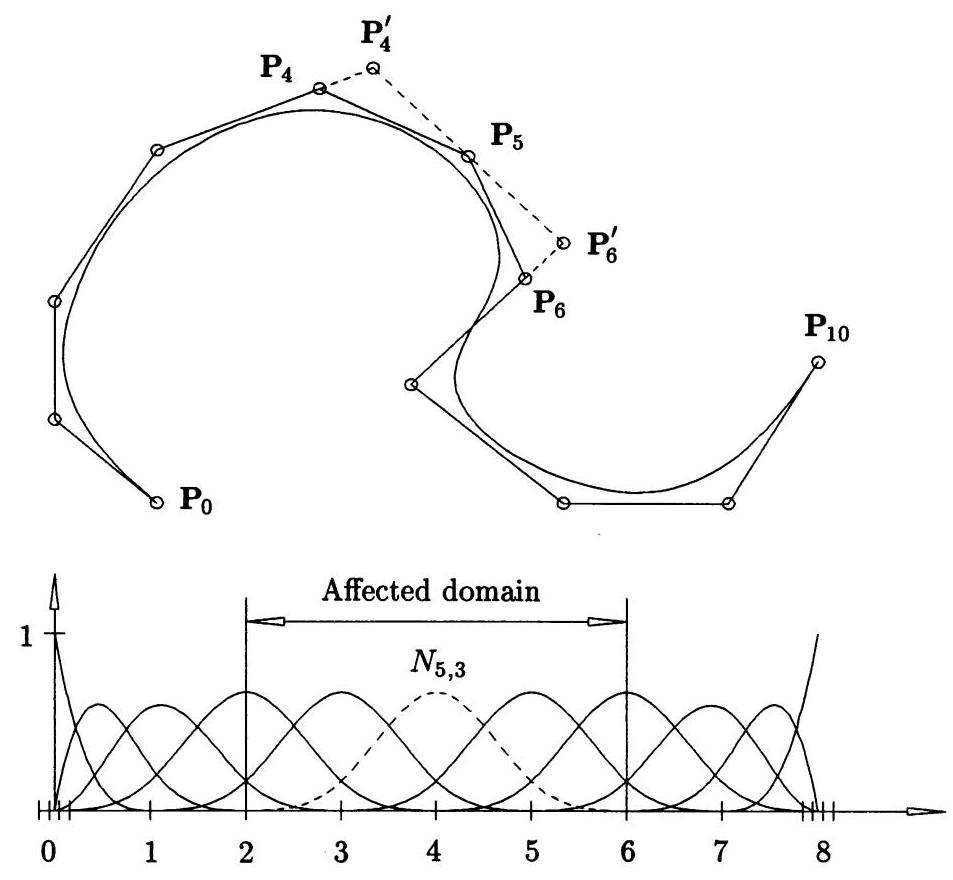
\includegraphics[max width=0.8\textwidth]{images/0193ba0d-ab19-7138-9798-cb281ce60de0_438_285_268_953_880_0.jpg}
\end{center}
\hspace*{3em} 

图 9.49. 移除结点 \({u}_{7} = 4\) 一次。

我们现在可以组合一个类型 2 曲线逼近方法。

算法 A9.10

\(\texttt{GlobalCurveApproxErrBnd(m,Q,P,E,n,U,P)}\)

\{ /* 全局曲线逼近到界限 E 内 */

/* 输入:m, Q, p, E */

/* 输出:n, U, P */

计算 \({\bar{u}}_{k}\) 并加载到 \(\mathrm{{ub}}\left\lbrack  \right\rbrack\) 中(公式 [9.5])。

将 \(U\) 和 \(P\) 设置为插值 \({Q}_{k}\) 的 1 次曲线: \(U = \left\{  {0,0,{\bar{u}}_{1},\ldots ,{\bar{u}}_{m - 1},1,1}\right\}\) 和 \({\mathbf{P}}_{k} = {\mathbf{Q}}_{k}\) 。

初始化 \({e}_{k} : \mathrm{{ek}}\left\lbrack  0\right\rbrack  ,\ldots ,\mathrm{{ek}}\left\lbrack  \mathrm{m}\right\rbrack   = 0\) 。

n = m;

for (deg=1; deg<=p; deg++)

\{

RemoveKnotsBoundCurve(n, p, U, P, ub, ek, E, nh, Uh, Ph);

if (deg == p) break;

设 \(U\) 为通过将 Uh 的度从 deg 提升到 deg+1(将所有重数增加 1)而获得的节点向量。重置 n(方程 [5.32])。

使用 \(\mathbf{n}\) 、ub、度 deg+1 和节点向量 U 对 \({\mathbf{Q}}_{k}\) 进行最小二乘曲线拟合；这将产生新的控制点 P。

\HRule

\hspace*{1em} Using Eqs. (6.4),(6.5), project all \({\mathbf{Q}}_{k}\) to current curve

\hspace*{4em} to get \({\mathbf{R}}_{k} = \mathbf{C}\left( {u}_{k}\right)\) . Then update ek[] and ub[]:

\hspace*{4em} \({e}_{k} = \left| {{\mathbf{Q}}_{k},{\mathbf{R}}_{k}}\right|\) and \({\bar{u}}_{k} = {u}_{k}.\)

\hspace*{1em} \} /* End of for-loop */

if \(\left( {n =  = {nh}}\right) \;\operatorname{return}\left( {n,U,P}\right)\) ;

Set \(U = {Uh}\) and \(n = {nh}\) , and fit one final time with degree \(p\)

\hspace*{3em} and knots U.

Project the \({\mathbf{Q}}_{k}\) and update ek[] and ub[].

RemoveKnotsBoundCurve(n, p, U, P, ub, ek, E, nh, Uh, Ph);

return(nh, Uh, Ph);

\}

\HRule

从线性曲线开始并逐步提升到度 \(p\) 的优势有三:

\begin{itemize}
\item 数据中固有的几何特征(例如，尖点和曲率的不连续性)往往在适当的阶段被捕捉；如果已知数据是平滑的，则算法 A9.10 可以从度 2 开始(在进入 for 循环之前进行二次插值)；
\end{itemize}

\begin{itemize}
\item 逐步演变的曲线往往会“稳定”到自然参数化；
\end{itemize}

\begin{itemize}
\item 在全局拟合大量点时的一般规则是，度数越高，节点越多(插值是极限)，波动越严重；算法 9.10 在增加度数的同时减少节点跨度，从而倾向于减少最终曲线的波动。
\end{itemize}

图 9.50a 显示了使用算法 A9.10 的立方曲线拟合示例。容差为 \(E = 7/{100}\) 。图 \({9.50}\mathrm{\;b}\) 显示了该曲线的参数化，以及控制多边形。注意双节点和单节点的混合，正如交替接触和不接触的多边形边所显示的那样。图 9.51 显示了另一个立方曲线逼近的示例，具有 \(E = 8/{100}\) 。

在算法 A9.10 的节点移除步骤中，最大范数误差界限 \(E\) 是有保证的。最小二乘拟合所产生的误差保证小于或等于之前(移除节点曲线)的误差，从最小二乘的意义上讲。在实践中，它似乎在最大范数意义上总是更好。无论如何，最大范数误差可以在点投影步骤中轻松监控，当 \({e}_{k}\) 和 \({\bar{u}}_{k}\) 被更新时。

通过使用算法 A9.6 进行拟合，并将相关的 \({e}_{k}\) 初始化为 \(\infty\) 而不更新它(或其 \({\bar{u}}_{k}\) )，可以轻松地将约束纳入算法中。Lyche [Lych87,88] 使用了类似的节点移除技术用于曲线和曲面逼近以及数据减少。

可以开发一种类似的类型 2 曲面逼近方法。设

\[
\mathbf{S}\left( {u,v}\right)  = \mathop{\sum }\limits_{{i = 0}}^{n}\mathop{\sum }\limits_{{j = 0}}^{m}{N}_{i,p}\left( u\right) {N}_{j,q}\left( v\right) {\mathbf{P}}_{i,j}\;\left( {u,v}\right)  \in  \left\lbrack  {0,1}\right\rbrack   \times  \left\lbrack  {0,1}\right\rbrack
\]

为一个 (p, q) 次 B 样条曲面。假设 \({u}_{r}\) 是一个重数为 \(s\) 的 \(u\) 节点，

\begin{center}
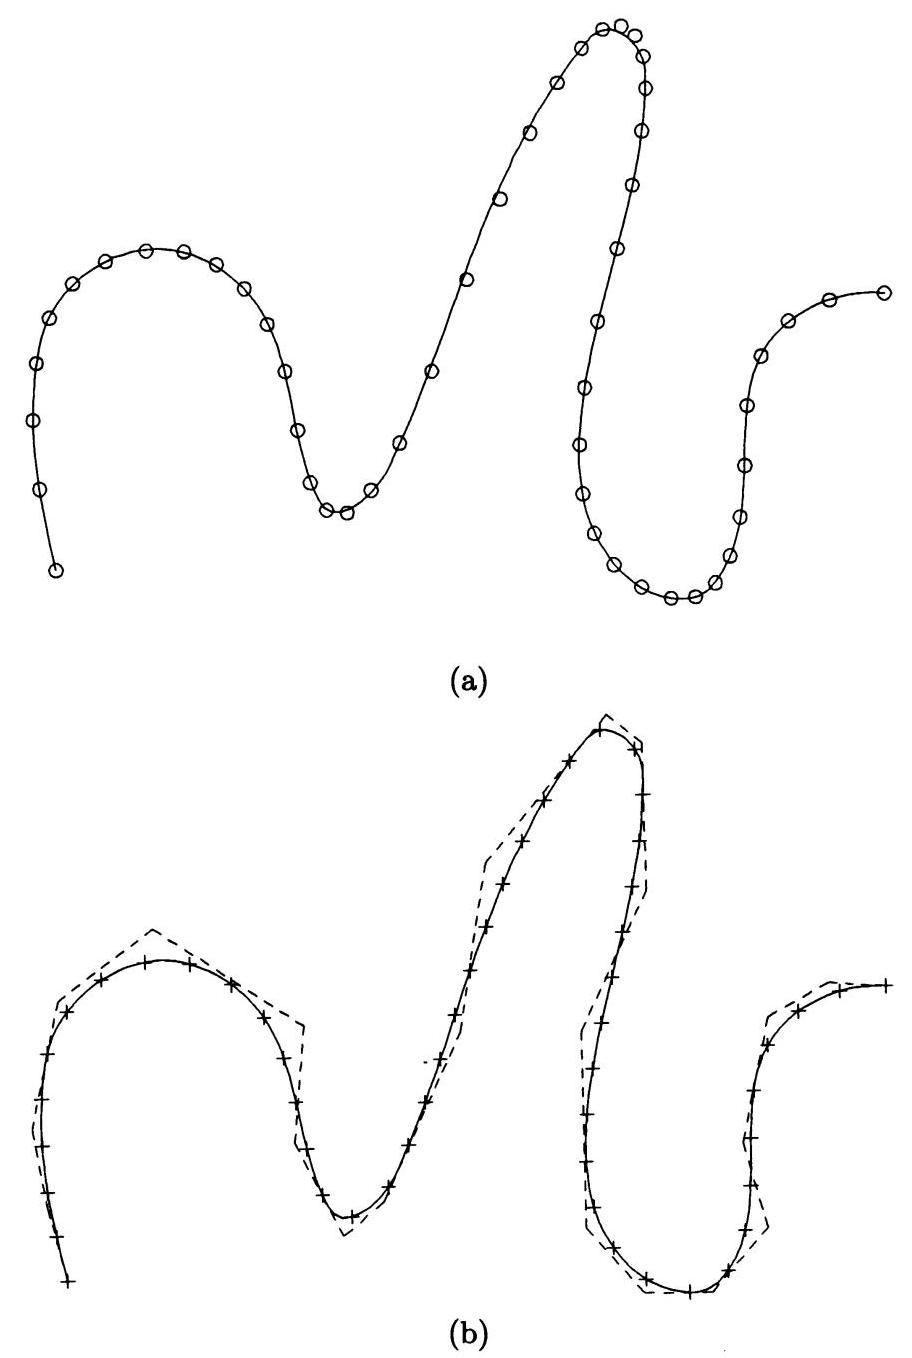
\includegraphics[max width=0.8\textwidth]{images/0193ba0d-ab19-7138-9798-cb281ce60de0_440_305_250_912_1358_0.jpg}
\end{center}
\hspace*{3em} 

图 9.50. 使用算法 A9.10 的立方曲线拟合。

并且让 \(\widehat{\mathbf{S}}\left( {u,v}\right)\) 表示通过移除一个 \({u}_{r}\) 的出现而获得的曲面。考虑到 \(\mathbf{S}\left( {u,v}\right)\) 的张量积结构，并使用 Tiller [Till92] 的技术，可以证明:

\[
\text{ - if }\left( {p + s}\right) {\;\operatorname{mod}\;2} = 0\text{ , set }k = \left( {p + s}\right) /2\text{ and }
\]

\[
{B}_{r}^{j} = \left| {{\mathbf{P}}_{r - k,j} - {\alpha }_{r - k}{\mathbf{P}}_{r - k + 1,j}^{1} - \left( {1 - {\alpha }_{r - k}}\right) {\mathbf{P}}_{r - k - 1,j}^{1}}\right|
\]

\[
j = 0,\ldots ,m \tag{9.86}
\]

其中

\[
{\alpha }_{r - k} = \frac{{u}_{r} - {u}_{r - k}}{{u}_{r - k + p + 1} - {u}_{r - k}}
\]

434 曲线与曲面拟合

\[
\text{ Then }\;\left| {\mathbf{S}\left( {u,v}\right)  - \widehat{\mathbf{S}}\left( {u,v}\right) }\right|  \leq  {N}_{r - k,p}\left( u\right) \mathop{\sum }\limits_{{j = 0}}^{m}{N}_{j,q}\left( v\right) {B}_{r}^{j}
\]

\[
\text{ for }\left( {u,v}\right)  \in  \left\lbrack  {0,1}\right\rbrack   \times  \left\lbrack  {0,1}\right\rbrack   \tag{9.87}
\]

\begin{center}
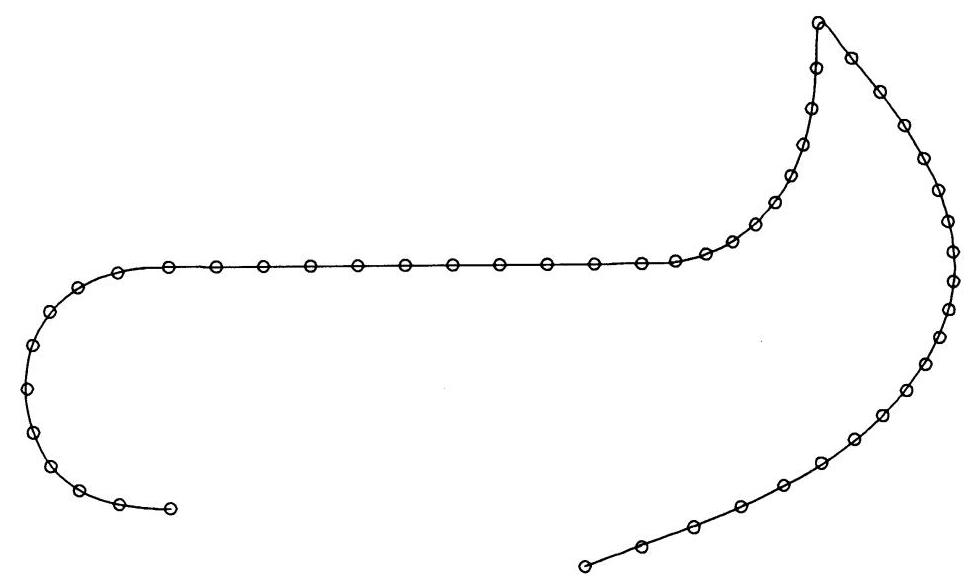
\includegraphics[max width=0.8\textwidth]{images/0193ba0d-ab19-7138-9798-cb281ce60de0_441_276_250_974_588_0.jpg}
\end{center}
\hspace*{3em} 

图 9.51. 使用算法 A9.10 和 \(E = 8/{100}\) 的立方曲线拟合。

\begin{itemize}
\item 如果 \(\left( {p + s}\right) {\;\operatorname{mod}\;2} = 1\) ，设置 \(k = \left( {p + s + 1}\right) /2\) 和
\end{itemize}

\[
{B}_{r}^{j} = \left| {{\mathbf{P}}_{r - k,j}^{1} - {\mathbf{P}}_{r - k + 1,j}^{1}}\right| \;j = 0,\ldots ,m \tag{9.88}
\]

\[
\text{ Then }\left| {\mathbf{S}\left( {u,v}\right)  - \widehat{\mathbf{S}}\left( {u,v}\right) }\right|  \leq  \left( {1 - {\alpha }_{r - k + 1}}\right) {N}_{r - k + 1,p}\left( u\right) \mathop{\sum }\limits_{{j = 0}}^{m}{N}_{j,q}\left( v\right) {B}_{r}^{j}
\]

\[
\text{ for }\left( {u,v}\right)  \in  \left\lbrack  {0,1}\right\rbrack   \times  \left\lbrack  {0,1}\right\rbrack   \tag{9.89}
\]

与

\[
{\alpha }_{r - k + 1} = \frac{{u}_{r} - {u}_{r - k + 1}}{{u}_{r - k + p + 2} - {u}_{r - k + 1}}
\]

类似的方程适用于 \(v\) 方向的结去除。利用这些方程，可以为类似于算法 A9.8 和 A9.9 的表面开发结去除策略。结合基于最小二乘的表面拟合算法 A9.7，提供了一种将一组点 \(\left\{  {\mathbf{Q}}_{k,\ell }\right\}\) 逼近到 \(E\) 容差内的方法。

图 \({9.52}\mathrm{a} - {9.52}\mathrm{e}\) 显示了几个表面逼近的例子。待逼近的数据集显示在图 9.52a 中。图 9.52b 显示了一个度数为 (2,2) 的表面，这是通过使用 \(E = 0\) 获得的插值面。将 \(E\) 增加到 \(1/2\) 会产生图 \({9.52}\mathrm{c}\) 中的表面。进一步将 \(E\) 增加到 1 会产生图 \({9.52}\mathrm{\;d}\) 中的表面。最后，使用 \(E = 1\) 的度数为 (3,3) 的逼近显示在图 9.52e 中。436 曲线和表面拟合

\begin{center}
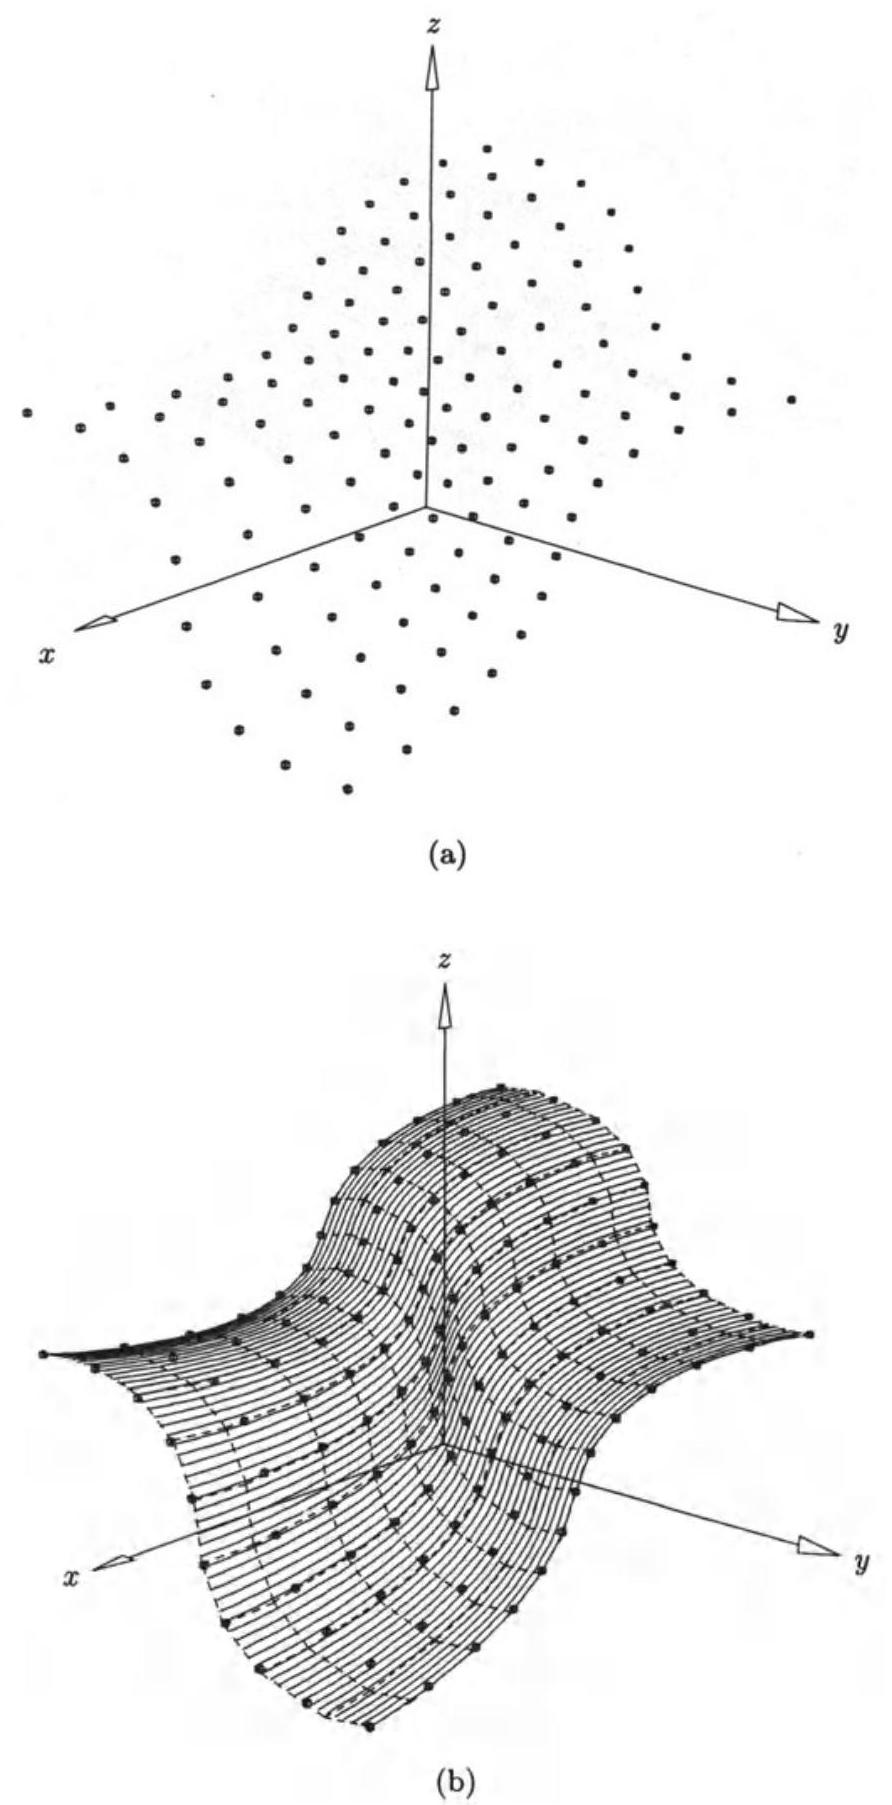
\includegraphics[max width=0.8\textwidth]{images/0193ba0d-ab19-7138-9798-cb281ce60de0_442_323_260_892_1805_0.jpg}
\end{center}
\hspace*{3em} 

图 9.52. 使用算法 A9.10 扩展到表面的各种表面拟合示例。

\begin{center}
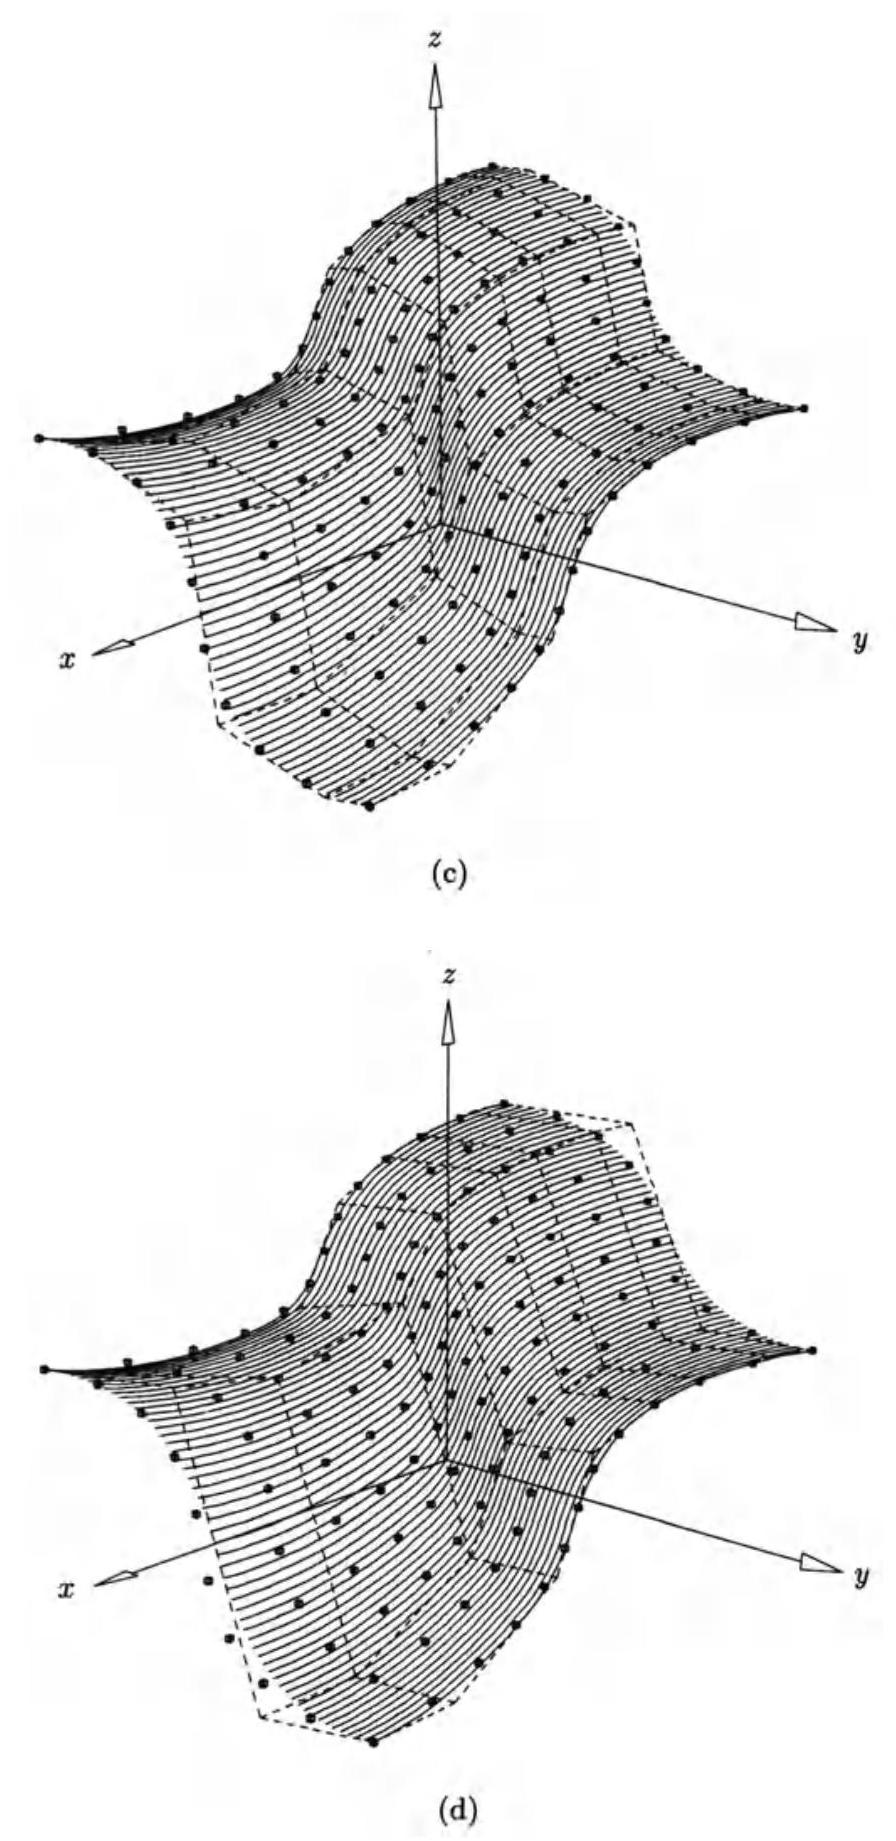
\includegraphics[max width=0.8\textwidth]{images/0193ba0d-ab19-7138-9798-cb281ce60de0_443_398_241_896_1841_0.jpg}
\end{center}
\hspace*{3em} 

图 9.52. (续。)

\begin{center}
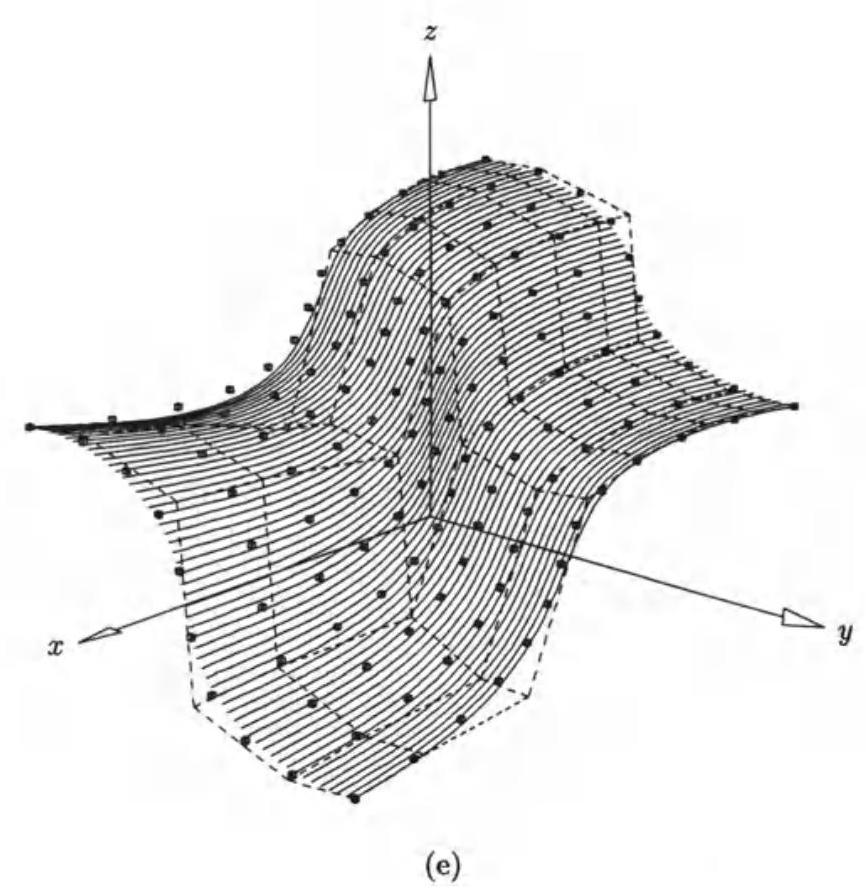
\includegraphics[max width=0.7\textwidth]{images/0193ba0d-ab19-7138-9798-cb281ce60de0_444_343_255_866_891_0.jpg}
\end{center}
\hspace*{3em} 

图 9.52. (续。)

算法 A9.10 和相应的表面算法实际上是数据简化算法，即它们在大数据集上效果最佳。它们假设在结去除阶段(算法 A9.9)可以去除大量结。如果情况并非如此，最小二乘逼近步骤可能会失败，原因可能是度数提升需要的控制点超过数据点，或者因为多个结使得方程组奇异。一个简单的解决方法是用更高阶的曲线重新开始该过程。



\section{局部逼近}

设定 \({\mathbf{Q}}_{0},\ldots ,{\mathbf{Q}}_{m}\) 和 \(E\) 。在这里，我们给出两个局部曲线近似的例子；第一个生成一个有理二次 B-spline 曲线，第二个生成一个非有理三次 B-spline 曲线。在这两种情况下，曲线都是通过构造而连续的 \({G}^{1}\) ；它们可以被设定为 \({C}^{1}\) 连续，但对于二次情况并不推荐这样做，因为这可能导致非常糟糕的参数化。二次曲线拟合平面数据，而三次曲线拟合任意三维数据。这些算法是对 [Pieg87b; Chou92] 中提出的方法的变体。

一个好的近似算法试图生成尽可能少的段。实现这一目标的一种方法是设定 \({k}_{s} = 0\) ，然后找到最大的 \({k}_{e} \leq  m\) ，使得 \({\mathbf{Q}}_{{k}_{s}},\ldots ,{\mathbf{Q}}_{{k}_{e}}\) 可以在 \(E\) 容差内通过一个 \(p\) 次段进行拟合。一旦找到，设定 \({k}_{s} = {k}_{e}\) 并重复该过程以找到最大的 \({k}_{e} \leq  m\) ，使得 \({\mathbf{Q}}_{{k}_{s}},\ldots ,{\mathbf{Q}}_{{k}_{e}}\) 可以通过一个 \(p\) 次段进行拟合。这一过程持续进行，直到 \({k}_{s} = m\) 。由于在近似中 \(m\) 通常相当大，因此二分搜索比线性搜索快得多。在实际操作中，可能希望限制可以通过一个段进行近似的数据点数量。我们用 \({K}_{\max }\) 表示这个界限，即，二分搜索算法被修改以保证

\[
{k}_{e} - {k}_{s} \leq  {K}_{\max }
\]

始终成立。这是通过在每次搜索下一个段的开始时将 \({k}_{e}\) 初始化为 \({k}_{s} + {K}_{\max }\) 来实现的。设定 \({K}_{\max } < m\) 有两个优点:

\begin{itemize}
\item 对于固定的容差 \(E\) ，较小的 \({K}_{\max }\) 产生更准确的拟合；
\end{itemize}

\begin{itemize}
\item 如果 \(m\) 很大而 \(E\) 非常小(这通常是情况)，那么每个段近似的点的平均数量相对于 \(m\) 是小的；在这种情况下，如果 \({K}_{\max }\) 设置得远小于 \(m\) ，算法将更有效。
\end{itemize}

我们在第 9.5.1 节和第 9.5.2 节中分别开发了 FitWithConic(   ) 和 FitWithCubic(   ) 例程。这些例程试图将点 \({\mathbf{Q}}_{{k}_{s}},\ldots ,{\mathbf{Q}}_{{k}_{e}}\) 拟合到容差 \(E\) 内，分别使用圆锥或立方段。如果拟合成功，调用(搜索)例程要么接受该段，要么增加 \({k}_{e}\) 并再次调用拟合例程以尝试找到更大的段(具体取决于搜索策略)。如果拟合不成功，调用例程将减少 \({k}_{e}\) 并再次调用拟合例程。

对于二次和三次情况，节点向量在接受段时构建。在这两种情况下都使用双内部节点，产生 \({G}^{1}\) 二次曲线和 \({C}^{1}\) 三次曲线。与段边界对应的累积弦长用于二次曲线的节点值；使用公式 (9.37) 计算三次曲线的节点。



\subsection{局部有理二次曲线逼近}

现在我们开发例程 FitWithConic(   )。我们假设点 \({\mathbf{Q}}_{{k}_{s}},\ldots ,{\mathbf{Q}}_{{k}_{e}}\) 位于唯一的平面中，并且给定了端切线 \({\mathbf{T}}_{s}\) 和 \({\mathbf{T}}_{e}\) 。

考虑图 9.53。暂时假设

\[
\mathbf{R} = {\mathbf{Q}}_{{k}_{s}} + {\gamma }_{s}{\mathbf{T}}_{s}\;\mathbf{R} = {\mathbf{Q}}_{{k}_{e}} + {\gamma }_{e}{\mathbf{T}}_{e} \tag{9.90}
\]

具有

\[
{\gamma }_{s} > 0\;{\gamma }_{e} < 0 \tag{9.91}
\]

然后确定一个近似的圆锥，分三步进行:

\begin{center}
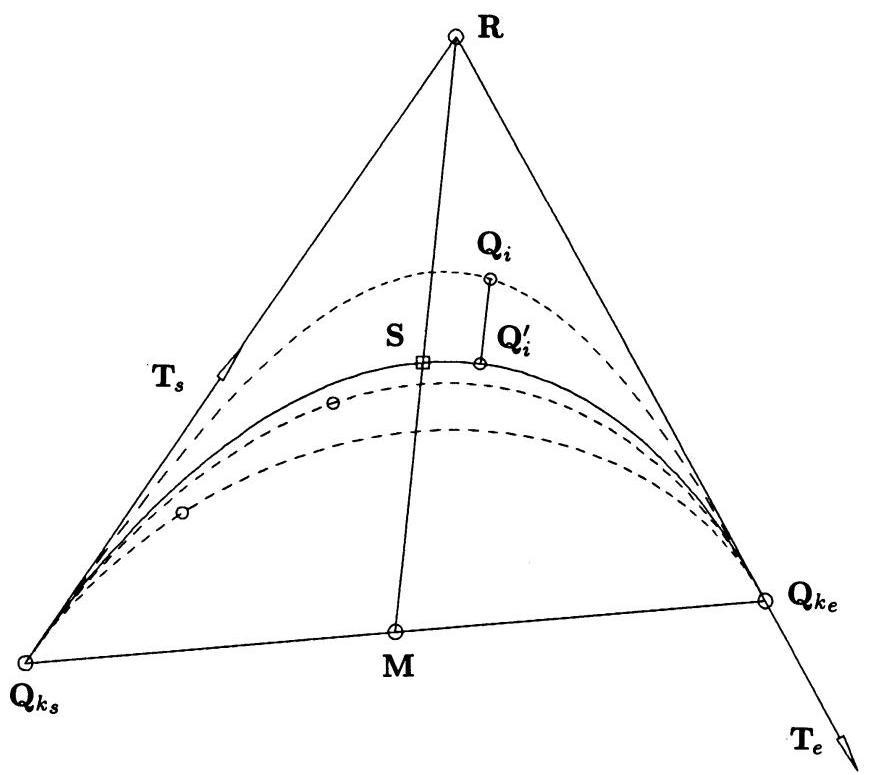
\includegraphics[max width=0.7\textwidth]{images/0193ba0d-ab19-7138-9798-cb281ce60de0_446_344_243_869_775_0.jpg}
\end{center}
\hspace*{3em} 

图 9.53. 圆锥曲线拟合的曲线拟合和散点检查。

1. 使用 \({\mathbf{Q}}_{{k}_{s}}\) 、 \(\mathbf{R}\) 和 \({\mathbf{Q}}_{{k}_{e}}\) 作为控制多边形，按照算法 A7.2 对每个点 \({\mathbf{Q}}_{i},i = {k}_{s} + 1,\ldots ,{k}_{e} - 1\) 进行插值。这将产生中间权重 \({w}_{i}\) 和相应的肩点坐标 \({s}_{i} = {w}_{i}/\left( {1 + {w}_{i}}\right)\) 。

2. 通过对 \({s}_{i}\) 进行平均计算一个近似圆锥，即。

\[
s = \frac{1}{{k}_{e} - {k}_{s} - 1}\mathop{\sum }\limits_{{i = {k}_{s} + 1}}^{{{k}_{e} - 1}}{s}_{i} \tag{9.92}
\]

根据公式 (7.30)，近似圆锥的肩点为 \(\mathbf{S} =\)  \(\left( {1 - s}\right) \mathbf{M} + s\mathbf{R}\) ，根据公式 (7.31)，中间权重为 \(w = s/\left( {1 - s}\right)\) ；

3. 将每个 \({\mathbf{Q}}_{i}\) 投影到近似圆锥上，以检查它们是否都在容差范围内。

有三种特殊情况需要不同处理:

\begin{itemize}
\item \({k}_{e} - {k}_{s} = 1\) ，即没有内部点；算法在 \({\mathbf{Q}}_{{k}_{s}}\) 和 \({\mathbf{Q}}_{{k}_{e}}\) 之间计算一个插值线段，正如第 9.3.3 节所描述的那样；
\end{itemize}

\begin{itemize}
\item \({\mathbf{T}}_{s}\) 和 \({\mathbf{T}}_{e}\) 是平行的；如果它们与弦 \({\mathbf{Q}}_{{k}_{s}}{\mathbf{Q}}_{{k}_{e}}\) 平行，并且点 \({\mathbf{Q}}_{{k}_{s}},\ldots ,{\mathbf{Q}}_{{k}_{e}}\) 共线，则返回的圆锥段实际上是一个线段；否则不进行拟合；
\end{itemize}

\begin{itemize}
\item 计算了 \(\mathbf{R}\) ，但公式 (9.91) 不成立；不进行拟合。
\end{itemize}

FitWithConic( ) 返回值 1 表示拟合成功，返回值 0 表示未进行拟合。在成功拟合的情况下，还返回加权中间控制点 \({\mathbf{R}}^{w}\) 。

\HRule

ALGORITHM A9.11

\hspace*{2em} FitWithConic(ks, ke, Q, Ts, Te, E, Rw)

\hspace*{4em} \{ /* Fit to tolerance E with conic segment */

\hspace*{6em} /* Input: ks, ke, Q, Ts, Te, E */

\hspace*{6em} /* Output: Rw */

\hspace*{4em} if (ke-ks == 1)

\hspace*{5em} \{ /* No interior points to interpolate */

\hspace*{5em} Fit an interpolating segment as in Section 9.3.3.

\hspace*{5em} return(1);

\hspace*{5em} \}

\hspace*{4em} i = Intersect3DLines(Q[ks], Ts, Q[ke], Te, alf1, alf2, R);

\hspace*{4em} if (i != 0 )

\hspace*{5em} \{ /* No intersection */

\hspace*{5em} if \(\left( {{\mathbf{Q}}_{{k}_{s}},\ldots ,{\mathbf{Q}}_{{k}_{e}}}\right.\) not collinear) return (0);

\hspace*{7em} else

\hspace*{9em} \{

\hspace*{9em} \(\mathrm{{Rw}} = \left( {\mathrm{Q}\left\lbrack  \mathrm{{ks}}\right\rbrack   + \mathrm{Q}\left\lbrack  \mathrm{{ke}}\right\rbrack  }\right) /{2.0};\)

\hspace*{9em} return(1);

\hspace*{9em} \}

\hspace*{5em} \}

\hspace*{4em} if (alf1 <= 0.0 || alf2 >= 0.0) return(0);

\hspace*{4em} s = 0.0; v = Q[ke]-Q[ks];

\hspace*{4em} for (i=ks+1; i<=ke-1; i++)

\hspace*{6em} \{ /* Get conic interpolating each interior point */

\hspace*{5em} V1 = Q[i] - R;

\hspace*{5em} j = Intersect3DLines(Q[ks], V, R, V1, alf1, alf2, dummy);

\hspace*{5em} if (j != 0 || alf1 <= 0.0 || alf1 >= 1.0 || alf2 <= 0.0)

\hspace*{7em} return(0);

\hspace*{5em} Compute the weight wi. /* Algorithm A7.2 */

\hspace*{5em} s = s + wi/(1.0+wi);

\hspace*{5em} \}

\hspace*{4em} \(\mathrm{s} = \mathrm{s}/\left( {\mathrm{{ke}} - \mathrm{{ks}} - 1}\right) ;\;\mathrm{w} = \mathrm{s}/\left( {{1.0} - \mathrm{s}}\right)\) ;

\hspace*{4em} if (w < WMIN || w > WMAX) /* system bounds on weights */

\hspace*{5em} return(0);

\hspace*{4em} Create Bezier segment with \(Q\left\lbrack  {ks}\right\rbrack  ,R,Q\left\lbrack  {ke}\right\rbrack\) and \(w\) .

\hspace*{4em} for (i=ks+1; i<=ke-1; i++)

\hspace*{5em} \{

\hspace*{5em} Project Q[i] onto the Bezier segment.

\hspace*{5em} if (distance > E) return(0);

\hspace*{5em} \}

\hspace*{4em} \({\mathrm{R}}_{\mathrm{W}} = \mathrm{w} * \mathrm{R}\) ;

\hspace*{4em} return(1);

\hspace*{3em} \}

\HRule

图 9.54a-9.54e 显示了局部二次曲线拟合的示例。对数螺旋

\[
r = \frac{1}{2}{e}^{\theta /5}
\]

被采样并进行了近似。图 \({9.54}\mathrm{a} - {9.54}\mathrm{\;d}\) 的输入参数为:

图 \({9.54}\mathrm{a}\;E = 1/{100},\;{K}_{\max } = {50}\)

图 \({9.54}\mathrm{\;b}\;E = 1/{1000},\;{K}_{\max } = {50}\)

图 \({9.54}\mathrm{c}\;E = 1/{10},\;{K}_{\max } = 6\)

图 \({9.54}\mathrm{\;d}\;E = 1/{10},\;{K}_{\max } = {10}\)

图 9.54e 显示了图 9.54b 中曲线的参数化。



\subsection{局部非有理三次曲线逼近}

现在我们开发 FitWithCubic(   )。设 \({\mathbf{P}}_{0} = {\mathbf{Q}}_{{k}_{s}}\) 和 \({\mathbf{P}}_{3} = {\mathbf{Q}}_{{k}_{e}}\) 表示三次 Bézier 段的起点和终点， \({\mathbf{T}}_{s}\) 和 \({\mathbf{T}}_{e}\) 表示起始和结束单位切线(见图 9.55)。我们必须确定两个内部控制点 \({\mathbf{P}}_{1}\) 和 \({\mathbf{P}}_{2}\) 。设定

\[
{\mathbf{P}}_{1} = {\mathbf{P}}_{0} + \alpha {\mathbf{T}}_{s}\;{\mathbf{P}}_{2} = {\mathbf{P}}_{3} + \beta {\mathbf{T}}_{e}
\]

我们必须确定 \(\alpha\) 和 \(\beta\) 的值，使得由 \({\mathbf{P}}_{0},{\mathbf{P}}_{1},{\mathbf{P}}_{2},{\mathbf{P}}_{3}\) 定义的三次 Bézier 曲线在所有 \({\mathbf{Q}}_{k},{k}_{s} < k < {k}_{e}\) 的 \(E\) 容差范围内。如果 \({k}_{e} - {k}_{s} = 1\) ，那么理论上，任何 \(\alpha\) 和 \(\beta\) 都可以；然而，它们应该被选择为使得导数的大小与邻近的大小自然融合。使用公式 (9.29) 和练习 9.2，对于 \({\mathbf{Q}}_{{k}_{s}}\) 和 \({\mathbf{Q}}_{{k}_{e}}\) 的导数 \({\mathbf{D}}_{{k}_{s}}\) 和 \({\mathbf{D}}_{{k}_{e}}\) 的合理估计为

\[
{\mathbf{D}}_{{k}_{s}} = {\mathbf{V}}_{{k}_{s}}\;\text{ if }{k}_{s} = 0
\]

\[
{\mathbf{D}}_{j} = \frac{{c}_{j + 1} - {c}_{j}}{{c}_{j} - {c}_{j - 1}}{\mathbf{V}}_{j}\;j \neq  \{ 0,m\} \;j = {k}_{s}\text{ or }j = {k}_{e}
\]

\[
{\mathbf{D}}_{{k}_{e}} = {\mathbf{V}}_{{k}_{e}}\;\text{ if }{k}_{e} = m \tag{9.93}
\]

其中 \(\left\{  {c}_{j}\right\}\) 是累积弦长。然后设定

\[
\alpha  = \frac{\left| {\mathbf{D}}_{{k}_{s}}\right| }{3}\;\beta  =  - \frac{\left| {\mathbf{D}}_{{k}_{e}}\right| }{3} \tag{9.94}
\]

现在假设 \({k}_{e} - {k}_{s} > 1\) 。我们的算法由三个步骤组成:

1. 对于每个 \(k,{k}_{s} < k < {k}_{e}\) ，插值一个三次 Bézier 段到数据 \({\mathbf{P}}_{0},{\mathbf{T}}_{s},{\mathbf{Q}}_{k},{\mathbf{P}}_{3},{\mathbf{T}}_{e}\) ，从而获得一个 \({\alpha }_{k}\) 和一个 \({\beta }_{k}\) ；Bézier 段 \({\mathbf{C}}_{\mathbf{k}}\left( u\right)\) 定义在归一化区间 \(u \in  \left\lbrack  {0,1}\right\rbrack\) 上；

442 曲线和曲面拟合

\begin{center}
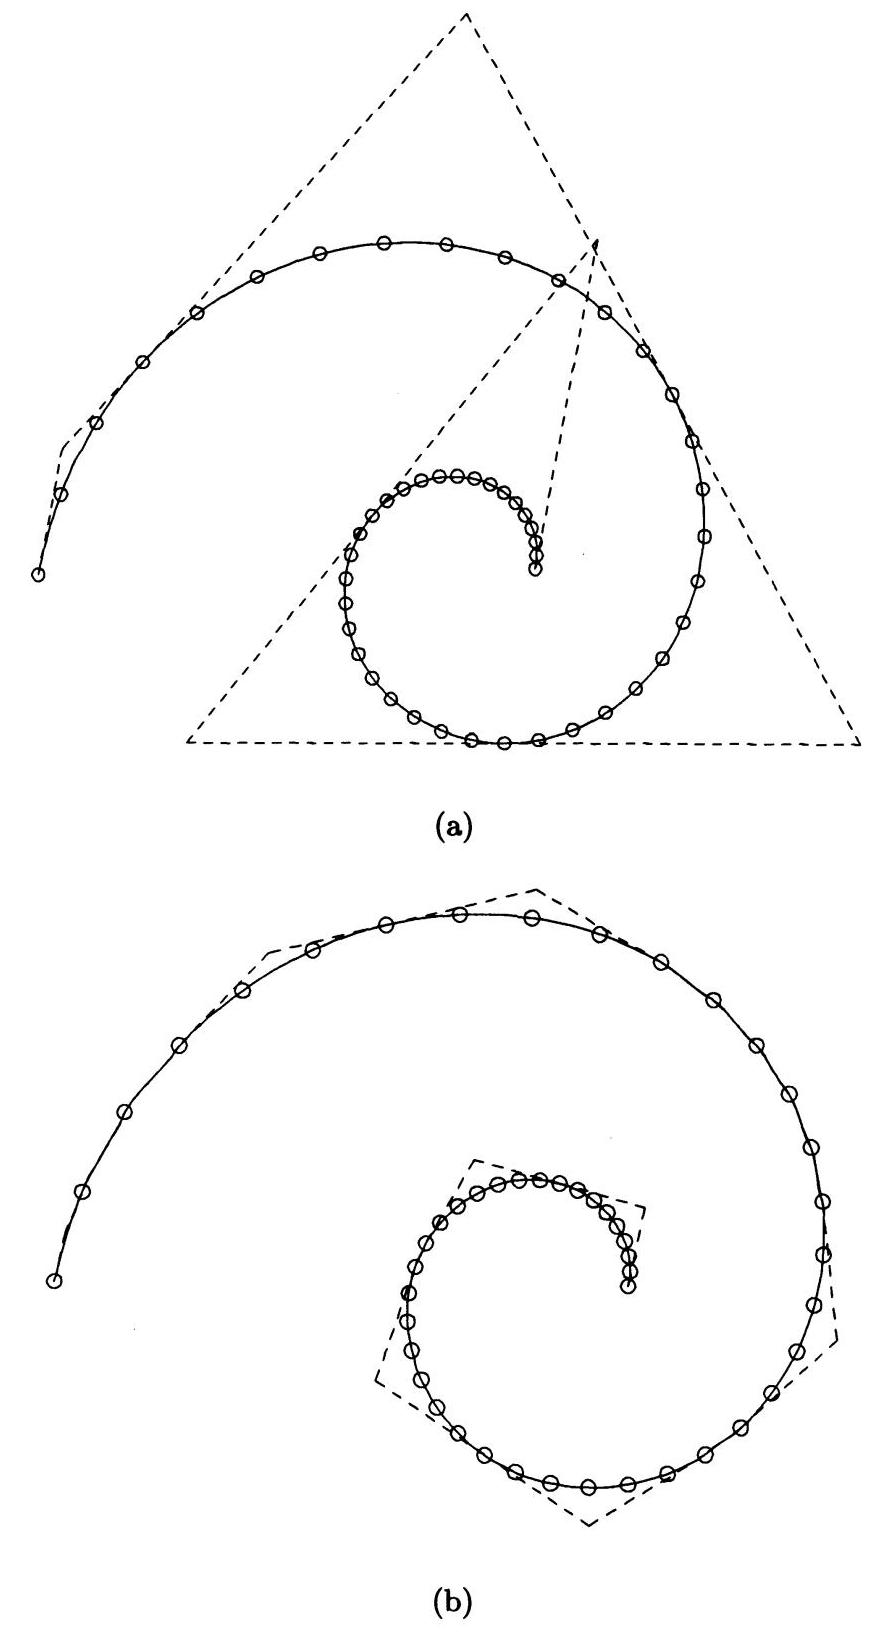
\includegraphics[max width=0.8\textwidth]{images/0193ba0d-ab19-7138-9798-cb281ce60de0_449_323_246_878_1634_0.jpg}
\end{center}
\hspace*{3em} 

图 9.54. 局部二次曲线拟合示例。

2. 对 \({\alpha }_{k}\mathrm{\;s}\) 和 \({\beta }_{k}\mathrm{\;s}\) 进行平均以获得 \(\alpha\) 和 \(\beta\) ；这些定义了候选的 Bézier 段， \(\mathbf{C}\left( u\right)\) ；

3. 检查所有 \({\mathbf{Q}}_{k},{k}_{s} < k < {k}_{e}\) 是否在 \(E\) 距离 \(\mathbf{C}\left( u\right)\) 之内。

\begin{center}
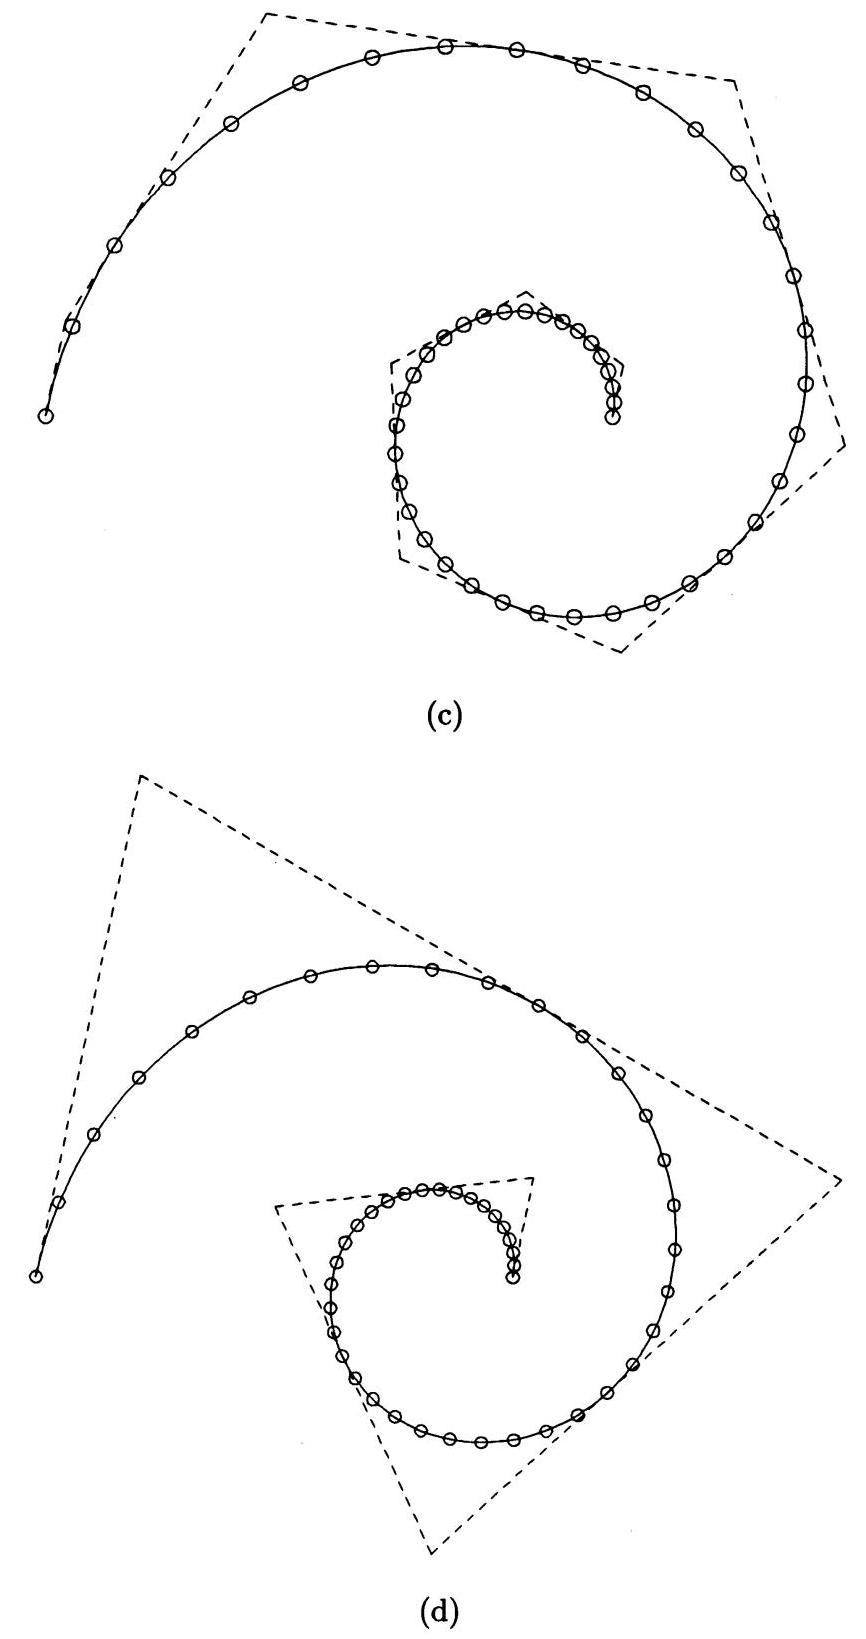
\includegraphics[max width=0.7\textwidth]{images/0193ba0d-ab19-7138-9798-cb281ce60de0_450_330_255_866_1639_0.jpg}
\end{center}
\hspace*{3em} 

图 9.54. (续。)

设 \(\mathbf{P} = {\mathbf{Q}}_{k}\) 为要插值的点，并用 \({B}_{i,3}\) 表示 \(u \in  \left\lbrack  {0,1}\right\rbrack\) 上的三次 Bernstein 多项式。我们写 \(\mathbf{P}\) 为

\[
\mathbf{P} = {B}_{0,3}{\mathbf{P}}_{0} + {B}_{1,3}{\mathbf{P}}_{1} + {B}_{2,3}{\mathbf{P}}_{2} + {B}_{3,3}{\mathbf{P}}_{3}
\]

444 曲线和曲面拟合

\[
= {\mathbf{P}}_{0}\left( {{B}_{0,3} + {B}_{1,3}}\right)  + \alpha {\mathbf{T}}_{s}{B}_{1,3} + \beta {\mathbf{T}}_{e}{B}_{2,3} + {\mathbf{P}}_{3}\left( {{B}_{2,3} + {B}_{3,3}}\right)  \tag{9.95}
\]

\begin{center}
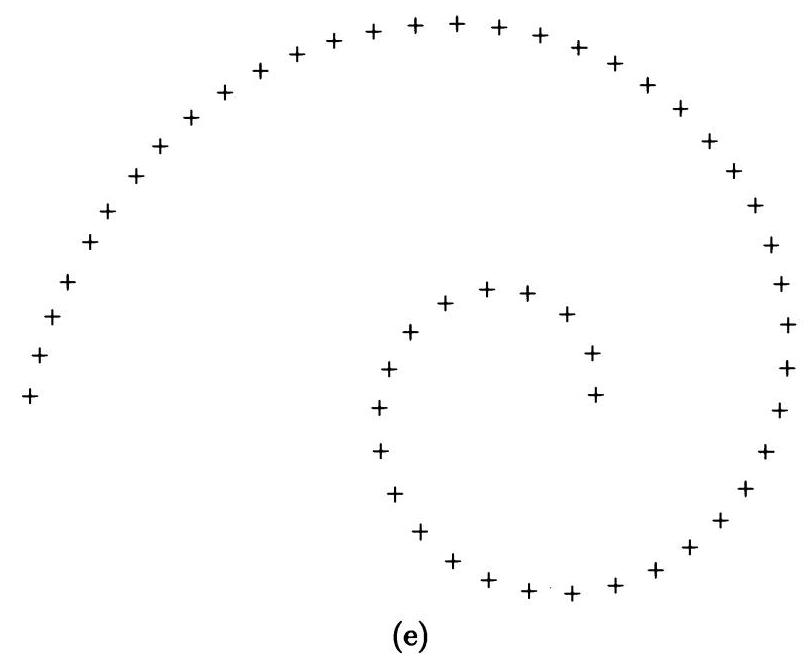
\includegraphics[max width=0.7\textwidth]{images/0193ba0d-ab19-7138-9798-cb281ce60de0_451_364_242_809_664_0.jpg}
\end{center}
\hspace*{3em} 

图 9.54. (续。)

最后

\[
\mathbf{P} = {\mathbf{P}}_{c} + a{\mathbf{T}}_{s} + b{\mathbf{T}}_{e} \tag{9.96}
\]

其中点

\[
{\mathbf{P}}_{c} = {\mathbf{P}}_{0}\left( {{B}_{0,3} + {B}_{1,3}}\right)  + {\mathbf{P}}_{3}\left( {{B}_{2,3} + {B}_{3,3}}\right)  \tag{9.97}
\]

位于直线 \({\mathbf{P}}_{0}{\mathbf{P}}_{3}\) 上，并

\[
a = \alpha {B}_{1,3}\;b = \beta {B}_{2,3} \tag{9.98}
\]

因此

\[
\alpha  = \frac{a}{{B}_{1,3}}\;\beta  = \frac{b}{{B}_{2,3}} \tag{9.99}
\]

考虑图 9.55。方程 (9.96) 表示我们通过从 \({\mathbf{P}}_{c}\) 开始，沿着与 \({\mathbf{T}}_{s}\) 平行的方向移动一定距离(到 \({\mathbf{P}}_{d}\) )，然后从那里继续朝着 \({\mathbf{T}}_{e}\) 的相反方向移动另一定距离，来获得 \(\mathbf{P}\) 。由于 \({\mathbf{T}}_{s}\) 和 \({\mathbf{T}}_{e}\) 的长度为单位，因此可以得出

\[
a = \left| {{\mathbf{P}}_{c}{\mathbf{P}}_{d}}\right| \;b =  - \left| {{\mathbf{P}}_{d}\mathbf{P}}\right|  \tag{9.100}
\]

因此，我们必须从方程 (9.100) 计算 \({\mathbf{P}}_{c}\) 和 \({\mathbf{P}}_{d}\) ，然后从方程 (9.100) 计算 \(a\) 和 \(b\) ，最后从方程 (9.99) 计算 \(\alpha\) 和 \(\beta\) 。

有两种情况需要考虑，平面内和不平面内。首先假设向量 \({\mathbf{T}}_{s},{\mathbf{T}}_{e}\) 和 \({\mathbf{P}}_{0}{\mathbf{P}}_{3}\) 不共面。事实证明，存在一条唯一的三次贝塞尔曲线通过 \(\mathbf{P}\) 、 \({\mathbf{P}}_{c}\) ，并且 \({\mathbf{P}}_{d}\) 可以按如下方式构造(见图 9.55):

\begin{center}
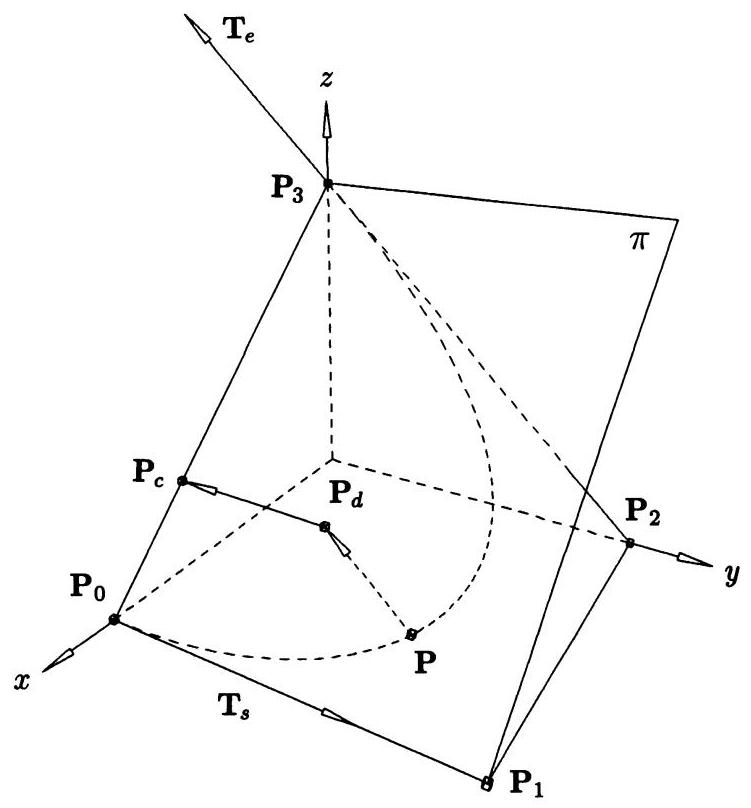
\includegraphics[max width=0.6\textwidth]{images/0193ba0d-ab19-7138-9798-cb281ce60de0_452_396_252_751_808_0.jpg}
\end{center}
\hspace*{3em} 

图 9.55。由端点、端切线和曲线上的一点指定的唯一三次三维(扭曲)贝塞尔曲线。

1. 设 \(\pi\) 为由 \({\mathbf{P}}_{0},{\mathbf{P}}_{3}\) 和 \({\mathbf{T}}_{s}\) 定义的平面；

2. 将 \(\pi\) 与通过 \(\mathbf{P}\) 并平行于 \({\mathbf{T}}_{e}\) 的直线相交 - 这将产生 \({\mathbf{P}}_{d}\) ；

3. 通过将直线 \({\mathbf{P}}_{0}{\mathbf{P}}_{3}\) 与通过 \({\mathbf{P}}_{d}\) 并平行于 \({\mathbf{T}}_{s}\) 的直线相交来获得 \({\mathbf{P}}_{c}\) 。

方程 (9.100) 现在得出 \(a\) 和 \(b\) 。为了通过方程 (9.99) 计算 \(\alpha\) 和 \(\beta\) ，我们需要唯一的参数值 \(\widehat{u}\) ，该值使得曲线通过点 P。从方程 (9.97) 和 \({B}_{i,3}\) 的和为 1 的事实，我们得到

\[
{\mathbf{P}}_{c} = \gamma {\mathbf{P}}_{0} + \left( {1 - \gamma }\right) {\mathbf{P}}_{3} \tag{9.101}
\]

其中

\[
\gamma  = \frac{\left| {\mathbf{P}}_{c}{\mathbf{P}}_{3}\right| }{\left| {\mathbf{P}}_{0}{\mathbf{P}}_{3}\right| } = {B}_{0,3} + {B}_{1,3} \tag{9.102}
\]

\(\gamma\) 被计算为定向距离的商，即 \(\gamma  \in  \left\lbrack  {0,1}\right\rbrack\) 当且仅当 \({\mathbf{P}}_{c}\) 位于 \({\mathbf{P}}_{0}\) 和 \({\mathbf{P}}_{3}\) 之间时。多项式 \({B}_{0,3} + {B}_{1,3}\) 在 \(u\) 中是三次的(读者应绘制此函数)，对于任何给定的 \(\gamma  \in  \left\lbrack  {0,1}\right\rbrack\) ，方程 (9.102) 有一个唯一的解位于 \(\left\lbrack  {0,1}\right\rbrack\) 内。如果 \(\gamma  \notin  \left\lbrack  {0,1}\right\rbrack\) ，则拟合被中止(返回“无拟合”给调用例程)。三次方程 (9.102) 可以通过牛顿迭代法求解。获得良好起始值的一种方法是列出一些与 0 到 1 之间的 \(\gamma\) 值对应的 \(\widehat{u}\) 值。然后，给定任何 \(\gamma\) ，在表中快速搜索可以得到一个起始 \(\widehat{u}\) 。最后，将 \(\widehat{u}\) 代入方程 (9.99) 得到 \(\alpha\) 和 \(\beta\) 。

如果 \({\mathbf{T}}_{s},{\mathbf{T}}_{e}\) 和 \({\mathbf{P}}_{0}{\mathbf{P}}_{3}\) 共面，则可以存在多条通过 \(\mathbf{P}\) 的立方曲线，而之前的几何构造 \({\mathbf{P}}_{c}\) 和 \({\mathbf{P}}_{d}\) 失效。有几个特殊情况使得问题复杂化，因此我们推导出一组方程，总是能得到 \(\alpha\) 和 \(\beta\) 。我们首先将一个参数 \(\widehat{u}\) 指派给 \(\mathbf{P}\) 。使用弦长参数化可以获得一个良好的估计，即。

\[
{\widehat{u}}_{{k}_{s}} = 0
\]

\[
{\widehat{u}}_{k} = {\widehat{u}}_{k - 1} + \frac{{c}_{k} - {c}_{k - 1}}{{c}_{{k}_{e}} - {c}_{{k}_{s}}} \tag{9.103}
\]

\({\widehat{u}}_{k}\) 实际上是 \({\mathbf{Q}}_{k}\) 在 \({\mathbf{Q}}_{{k}_{s}},\ldots ,{\mathbf{Q}}_{{k}_{e}}\) 上的标准化弦长参数。现在如果 \(\mathbf{P} = {\mathbf{Q}}_{k},{k}_{s} < k < {k}_{e}\) ，那么 \(\widehat{u} = {\widehat{u}}_{k}\) 。

接下来我们计算在 \(\mathbf{P}\) 处的切线 \({\mathbf{T}}_{p}\) (方程 [9.29] 和 [9.31])。设

\[
s = 1 - \widehat{u}\;t = \widehat{u}
\]

根据定义

\[
\mathbf{P} = {s}^{3}{\mathbf{P}}_{0} + 3{s}^{2}t{\mathbf{P}}_{1} + {3s}{t}^{2}{\mathbf{P}}_{2} + {t}^{3}{\mathbf{P}}_{3} \tag{9.104}
\]

并回忆 deCasteljau 算法(方程 [1.12]、算法 A1.5 和图 1.17)，可以推导出

\[
{\mathbf{P}}_{0}^{2} = {s}^{2}{\mathbf{P}}_{0} + {2st}{\mathbf{P}}_{1} + {t}^{2}{\mathbf{P}}_{2}
\]

\[
{\mathbf{P}}_{1}^{2} = {s}^{2}{\mathbf{P}}_{1} + {2st}{\mathbf{P}}_{2} + {t}^{2}{\mathbf{P}}_{3} \tag{9.105}
\]

其中 \({\mathbf{P}}_{0}^{2}\) 和 \({\mathbf{P}}_{1}^{2}\) 位于由 \(\mathbf{P}\) 和 \({\mathbf{T}}_{p}\) 定义的直线上(图 9.56)。因此

\[
0 = {\mathbf{T}}_{p} \times  \left( {{\mathbf{P}}_{1}^{2} - {\mathbf{P}}_{0}^{2}}\right)
\]

\[
= {\mathbf{T}}_{p} \times  \left( {{t}^{2}{\mathbf{P}}_{3} + t\left( {{2s} - t}\right) {\mathbf{P}}_{2} + s\left( {s - {2t}}\right) {\mathbf{P}}_{1} - {s}^{2}{\mathbf{P}}_{0}}\right)  \tag{9.106}
\]

将 \({\mathbf{P}}_{1} = {\mathbf{P}}_{0} + \alpha {\mathbf{T}}_{s}\) 和 \({\mathbf{P}}_{2} = {\mathbf{P}}_{3} + \beta {\mathbf{T}}_{e}\) 代入方程 (9.104) 和 (9.106) 得到

\[
\left( {3{s}^{2}t{\mathbf{T}}_{s}}\right) \alpha  + \left( {{3s}{t}^{2}{\mathbf{T}}_{e}}\right) \beta  = \mathbf{P} - \left( {{s}^{3} + 3{s}^{2}t}\right) {\mathbf{P}}_{0} - \left( {{t}^{3} + {3s}{t}^{2}}\right) {\mathbf{P}}_{3} \tag{9.107}
\]

\[
s\left( {s - {2t}}\right) \left( {{\mathbf{T}}_{p} \times  {\mathbf{T}}_{s}}\right) \alpha  + t\left( {{2s} - t}\right) \left( {{\mathbf{T}}_{p} \times  {\mathbf{T}}_{e}}\right) \beta  = {2st}\left( {{\mathbf{T}}_{p} \times  \left( {{\mathbf{P}}_{0} - {\mathbf{P}}_{3}}\right) }\right)  \tag{9.108}
\]

方程 (9.107) 涉及点约束 \(\mathbf{P}\) ，而方程 (9.108) 涉及切线约束 \({\mathbf{T}}_{p}\) 。它们各自对两个未知数贡献三个方程，总共六个方程(或者在数据为 \({xy}\) 平面时为四个)。一些特殊情况是:

\begin{itemize}
\item 如果 \({\mathbf{T}}_{s}\parallel {\mathbf{T}}_{e}\) ，则方程 (9.107) 仅产生一个方程；方程 (9.108) 提供必要的附加方程；
\end{itemize}

\begin{center}
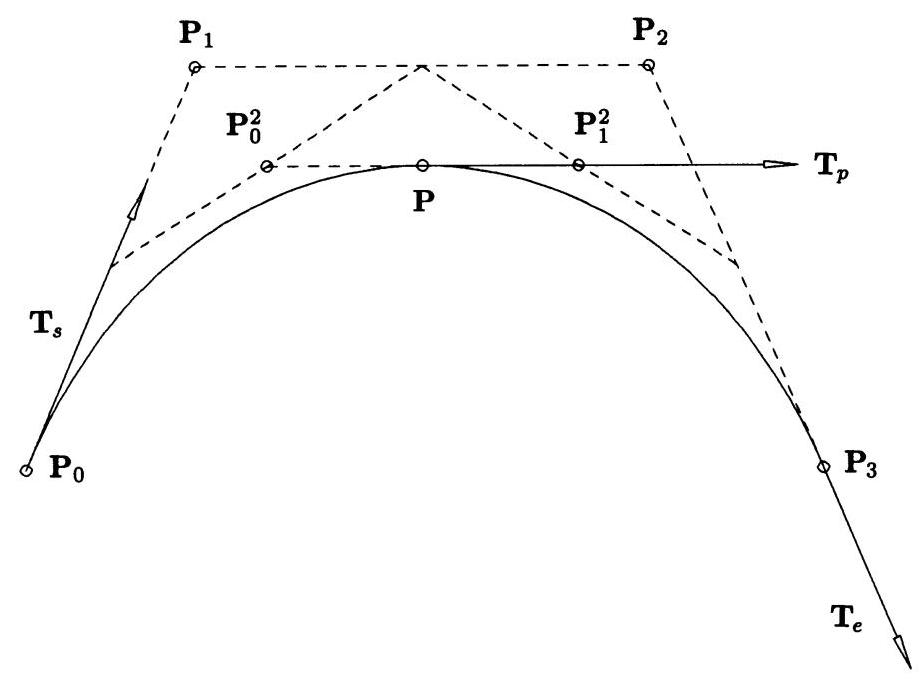
\includegraphics[max width=0.8\textwidth]{images/0193ba0d-ab19-7138-9798-cb281ce60de0_454_297_247_923_680_0.jpg}
\end{center}
\hspace*{3em} 

图 9.56. 由端点、端切线、曲线上的一点及该点的切线方向指定的平面立方 Bézier 曲线。

\begin{itemize}
\item 如果 \(\mathbf{P} = \left( {{s}^{3} + 3{s}^{2}t}\right) {\mathbf{P}}_{0} + \left( {{t}^{3} + {3s}{t}^{2}}\right) {\mathbf{P}}_{3}\) ，则方程 (9.107) 是一个齐次系统；在这种情况下， \(\alpha  = \beta  = 0\) 可能是唯一的解，或者可能存在无限多个非平凡解。假设我们已经排除了直线情况，我们有 \({\mathbf{T}}_{p} \times  \left( {{\mathbf{P}}_{0} - {\mathbf{P}}_{3}}\right)  \neq  0\) ，因此方程 (9.108) 提供了必要的非齐次方程。
\end{itemize}

一种简单的解决方程 (9.107) 和 (9.108) 的方法，避免了对特殊情况的担忧，是将六个方程组合在一起并通过最小二乘法求解。求解后，必须检查 \(\alpha  > 0\) 和 \(\beta  < 0\) 是否成立；如果不成立，则拟合被中止，控制权返回给调用程序。

一旦方程被求解， \({\alpha }_{k}\mathrm{\;s}\) 和 \({\beta }_{k}\mathrm{\;s}\) 仅需取平均，即

\[
\alpha  = \frac{1}{{k}_{e} - {k}_{s} - 1}\mathop{\sum }\limits_{{i = {k}_{s} + 1}}^{{{k}_{e} - 1}}{\alpha }_{i}\;\beta  = \frac{1}{{k}_{e} - {k}_{s} - 1}\mathop{\sum }\limits_{{i = {k}_{s} + 1}}^{{{k}_{e} - 1}}{\beta }_{i} \tag{9.109}
\]

候选立方 Bézier 曲线 \(\mathbf{C}\left( u\right)\) 由 \({\mathbf{P}}_{0},{\mathbf{P}}_{1} = {\mathbf{P}}_{0} + \alpha {\mathbf{T}}_{s}\) 、 \({\mathbf{P}}_{2} = {\mathbf{P}}_{3} + \beta {\mathbf{T}}_{e}\) 和 \({\mathbf{P}}_{3}\) 定义。

现在我们必须检查每个 \({\mathbf{Q}}_{k}\) 是否在曲线 \(\mathbf{C}\left( u\right)\)  \(\left( {{k}_{s} < k < {k}_{e}}\right)\) 的 \(E\) 距离内。这需要牛顿迭代，之前计算的 \(\widehat{u}\) 是良好的起始值。回想一下 \({\mathbf{Q}}_{k} = {\mathbf{C}}_{k}\left( {\widehat{u}}_{k}\right)\) 。设 \(\Delta {\alpha }_{k} = {\alpha }_{k} - \alpha\) 和 \(\Delta {\beta }_{k} = {\beta }_{k} - \beta\) 。然后从方程 (9.95) 我们得到

\[
\left| {{\mathbf{Q}}_{k} - \mathbf{C}\left( {\widehat{u}}_{k}\right) }\right|  = \left| {{\mathbf{C}}_{k}\left( {\widehat{u}}_{k}\right)  - \mathbf{C}\left( {\widehat{u}}_{k}\right) }\right|
\]

\[
= \left| {\Delta {\alpha }_{k}{B}_{1,3}\left( {\widehat{u}}_{k}\right) {\mathbf{T}}_{s} - \Delta {\beta }_{k}{B}_{2,3}\left( {\widehat{u}}_{k}\right) {\mathbf{T}}_{e}}\right|  \tag{9.110}
\]

方程 (9.110) 可以用作快速接受测试:如果它小于或等于 \(E\) ，则不需要牛顿迭代。如果需要迭代，则第 6.1 节中给出的技术是合适的。

FitWithCubic(   ) 的例程如下。它返回值 1 表示拟合成功，返回值 0 表示没有拟合。我们注意到，在非共面的情况下，当 \({\mathbf{T}}_{s},{\mathbf{T}}_{e}\) 和 \({\mathbf{P}}_{0}{\mathbf{P}}_{3}\) 接近共面时， \({\mathbf{P}}_{c}\) 和 \({\mathbf{P}}_{d}\) 的构造是不稳定的。因此，这个测试应该在相对宽松的容差下进行。该算法使用局部数组 uh[]、alfak[]、betak[] 来存储 \({\widehat{u}}_{k},{\alpha }_{k}\) 和 \({\beta }_{k}\) 。

\HRule

\section*{ALGORITHM A9.12}

\hspace*{1em} FitWithCubic(ks, ke, Q, Ts, Te, E, P1, P2)

\hspace*{3em} \{ /* Fit to tolerance E with cubic segment */

\hspace*{4em} /* Input: ks, ke, Q, Ts, Te, E */

\hspace*{4em} /* Output: P1, P2 */

\hspace*{2em} if (ke-ks == 1)

\hspace*{4em} \{ /* No interior points to interpolate */

\hspace*{4em} Compute \(\alpha\) and \(\beta\) by Eqs. (9.93),(9.94).

\hspace*{4em} Set \({\mathbf{P}}_{1} = {\mathbf{Q}}_{{k}_{s}} + \alpha {\mathbf{T}}_{s}\)

\hspace*{4em} and \({\mathbf{P}}_{2} = {\mathbf{Q}}_{{k}_{e}} + \beta {\mathbf{T}}_{e}\)

\hspace*{4em} return(1);

\hspace*{4em} \}

\hspace*{2em} dk = ke-ks;

\hspace*{2em} line = Collinear(dk+1, Q[ks]);

\hspace*{2em} if (line == 1)

\hspace*{4em} \{ /* Collinear points case; create straight line */

\hspace*{4em} P1 = (2.0*Q[ks]+Q[ke])/3.0;

\hspace*{4em} P2 = (Q[ks]+2.0*Q[ke])/3.0;

\hspace*{4em} return(1);

\hspace*{4em} \}

\hspace*{2em} for (k=1; k<dk; k++)

\hspace*{4em} \{

\hspace*{4em} Get plane \(\pi\) defined by \(Q\left\lbrack  {ks}\right\rbrack  ,Q\left\lbrack  {ke}\right\rbrack\) , Ts.

\hspace*{4em} if (Line(Q[k+ks], Te) lies in \(\pi\) )

\hspace*{5em} \{ /* Coplanar case */

\hspace*{5em} Compute \({\widehat{u}}_{k}\) by Eq. (9.103) and load into uh[k].

\hspace*{5em} Set up Eqs. (9.107) and (9.108) and solve for \({\alpha }_{k}\) and \({\beta }_{k}\)

\hspace*{7em} (by least squares).

\hspace*{5em} if \(\left( {{\alpha }_{k} > 0\text{ \&\& }{\beta }_{k} < 0}\right)\)

\hspace*{6em} \{

\hspace*{6em} \(\operatorname{alfak}\left\lbrack  \mathrm{k}\right\rbrack   = {\alpha }_{k};\;\) beta \(\mathrm{k}\left\lbrack  \mathrm{k}\right\rbrack   = {\beta }_{k};\)

\hspace*{6em} \}

\hspace*{6em} else

\hspace*{7em} return(0);

\hspace*{5em} \}

\hspace*{5em} else

\hspace*{5em} \{ /* Noncoplanar case */

\hspace*{5em} \(\mathrm{{Pd}} =\) Intersection of \(\pi\) with Line \(\left( {\mathrm{Q}\left\lbrack  {\mathrm{k} + \mathrm{{ks}}}\right\rbrack  ,\mathrm{{Te}}}\right)\) ;

\hspace*{5em} Pc = Intersection of Line(Q[ks], Q[ke]-Q[ks]) with

\hspace*{9em} Line(Pd, Ts);

\hspace*{5em} gamma = Distance3D(Pc, Q[ke])/Distance3D(Q[ks], Q[ke]);

\hspace*{5em} if \(\left( {\text{ gamma } < {0.0} \mid   \mid  \text{ gamma } > {1.0}}\right) \;\) return(0);

\hspace*{5em} Use Newton iteration to solve Eq. (9.102) for uh[k].

\hspace*{5em} if \(\left( {{uh}\left\lbrack  k\right\rbrack   < {0.0} \mid  {uh}\left\lbrack  k\right\rbrack   > {1.0}}\right)\) return(0);

\hspace*{7em} else

\hspace*{7em} \{

\hspace*{7em} \(a = \operatorname{Distance3D}\left( {{Pc},{Pd}}\right) ;\;b =  - \operatorname{Distance3D}\left( {{Pd},Q\left\lbrack  {k + {ks}}\right\rbrack  }\right) ;\)

\hspace*{7em} Evaluate Bernstein polynomials and use Eq. (9.99)

\hspace*{9em} to get alfak \(\left\lbrack  k\right\rbrack\) and beta \(k\left\lbrack  k\right\rbrack\) .

\hspace*{6em} \}

\hspace*{4em} \}

\hspace*{2em} \} /* End of for-loop: \(k = 1,\ldots ,{dk} - 1 * /\)

\hspace*{4em} /* Step 2: average the \({\alpha }_{k}\mathrm{\;s}\) and \({\beta }_{k}\mathrm{\;s} *\) /

alpha = beta = 0.0 ;

for ( \(k = 1\) ; \(k < {dk}\) ; \(k +  +\) )

\hspace*{3em} \{ alpha = alpha+alfak[k]; beta = beta+betak[k]; \}

alpha = alpha/(dk-1); beta = beta/(dk-1);

P1 = Q[ks]+alpha*Ts; P2 = Q[ke]+beta*Te;

\hspace*{4em} /* Step 3: check deviations */

for (k=1; k<dk; k++)

\hspace*{2em} \{

\hspace*{2em} \(\mathrm{u} = \operatorname{uh}\left\lbrack  \mathrm{k}\right\rbrack\) ;

\hspace*{2em} if (Eq. [9.110] less than E) continue;

\hspace*{5em} else

\hspace*{5em} \{ /* Must do Newton iterations. u is start value */

\hspace*{5em} Project \(Q\left\lbrack  {k + {ks}}\right\rbrack\) to curve to get error ek.

\hspace*{5em} if (ek > E) break;

\hspace*{4em} \}

\hspace*{2em} \}

if \(\left( {k =  = {dk}}\right) \;\) return \(\left( 1\right) ;\;\) /* segment within tolerance \(*\) /

\hspace*{3em} else return(0); /* not within tolerance */

\}

\HRule

图 9.57 和 9.58 分别展示了平面和非平面拟合的示例。图 9.57 的输入数据为

图 \({9.57}\mathrm{a}\;E = 1/{10},\;{K}_{\max } = {11}\)

图 \({9.57}\mathrm{\;b}\;E = 1/{10},\;{K}_{\max } = 8\)

图 \({9.57}\mathrm{c}\;E = 1/{100},\;{K}_{\max } = {11}\)

注意从图 9.57a 到图 9.57b 近似质量的变化。在相同的容差下，允许每个段最多八个点而不是十一点显著改善了近似效果。图 [latex0] 的输入数据为

\begin{center}
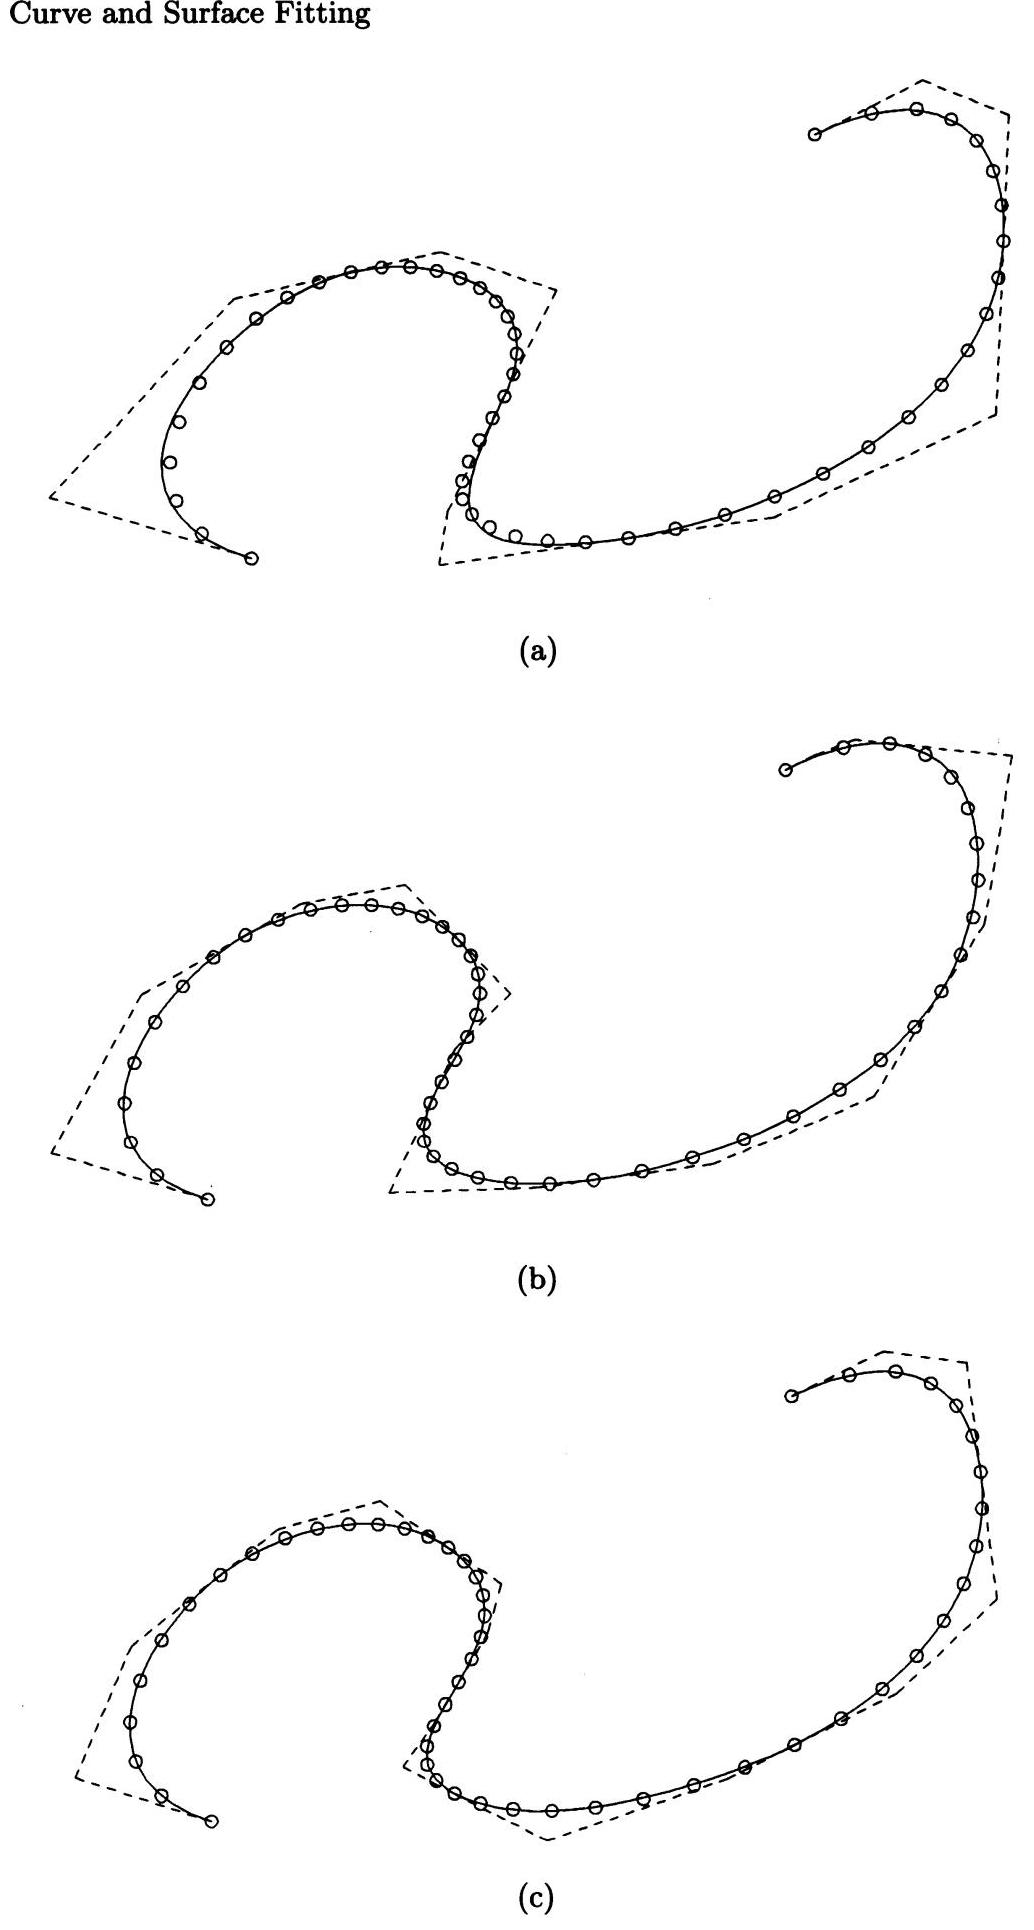
\includegraphics[max width=0.9\textwidth]{images/0193ba0d-ab19-7138-9798-cb281ce60de0_457_294_186_1034_1930_0.jpg}
\end{center}
\hspace*{3em} 

图 9.57. 对平面数据的局部三次近似。

\begin{center}
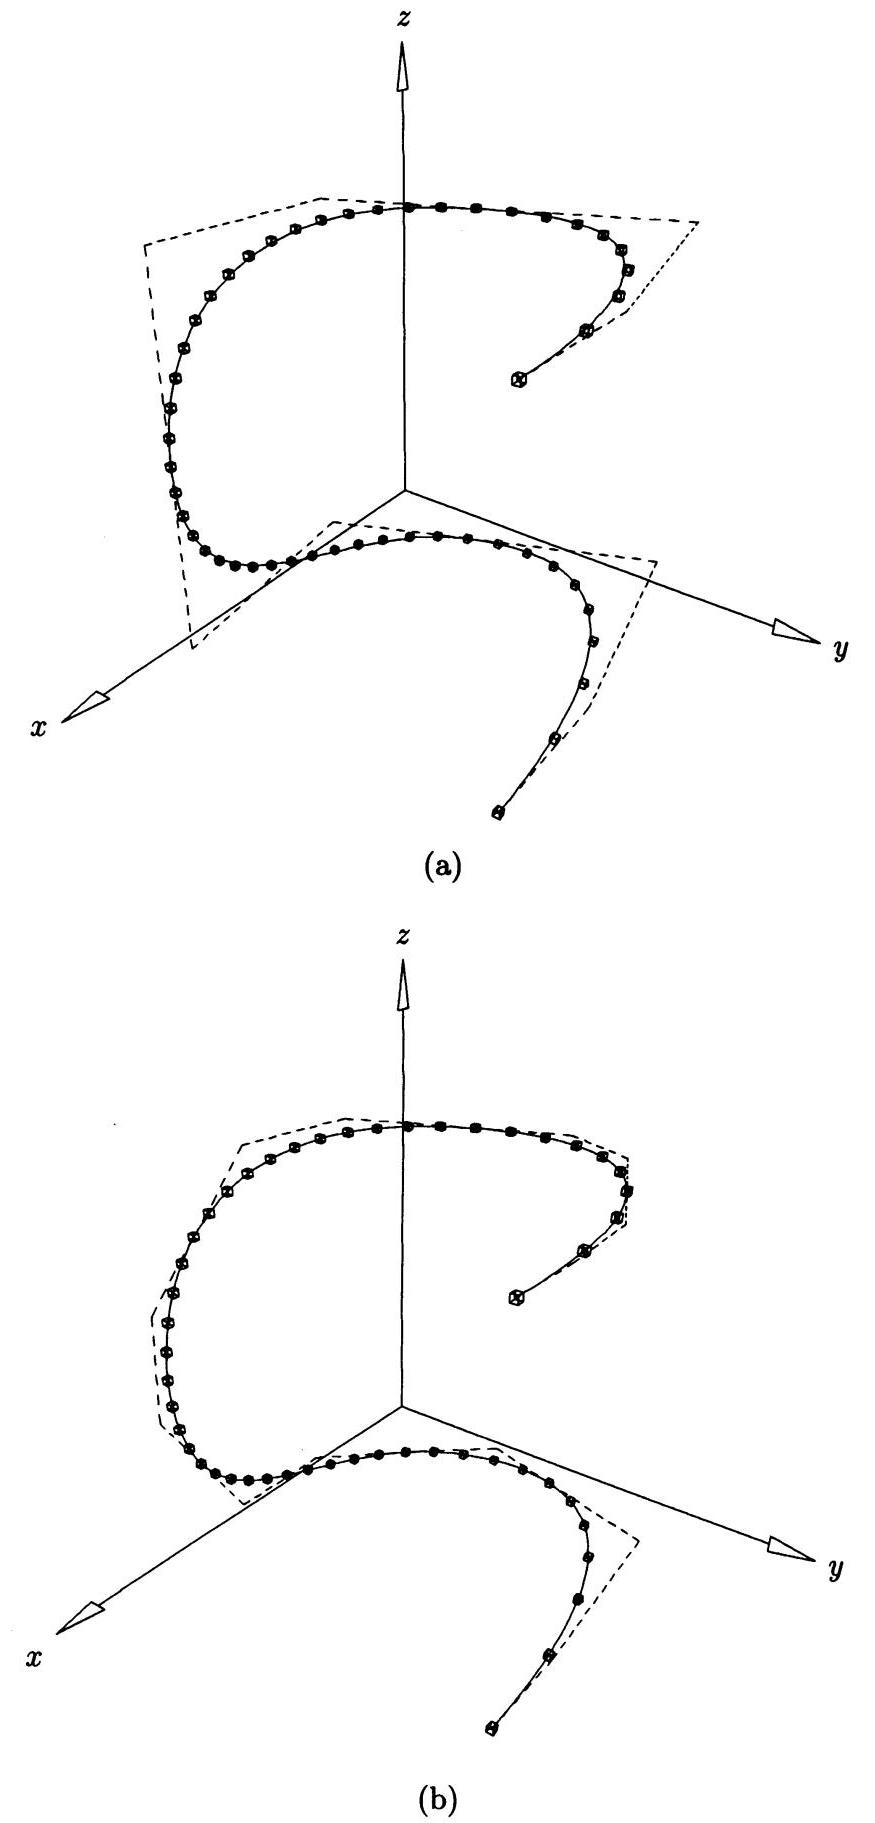
\includegraphics[max width=0.8\textwidth]{images/0193ba0d-ab19-7138-9798-cb281ce60de0_458_333_248_875_1823_0.jpg}
\end{center}
\hspace*{3em} 

图 9.58. 对包含平面段的三维数据的局部三次近似。

452 曲线和曲面拟合

\begin{center}
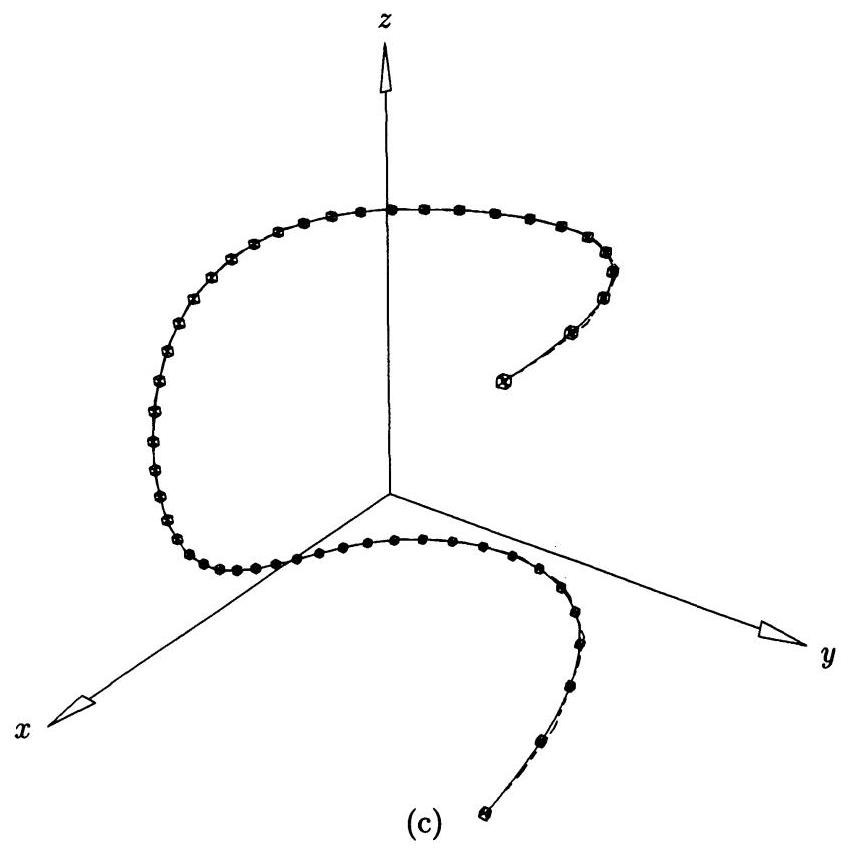
\includegraphics[max width=0.7\textwidth]{images/0193ba0d-ab19-7138-9798-cb281ce60de0_459_351_252_850_849_0.jpg}
\end{center}
\hspace*{3em} 

图 9.58. (续。)

图 \({9.58}\mathrm{a} - {9.58}\mathrm{c}\) 的输入数据为

图 \({9.58}\mathrm{a}\;E = 1/{10},\;{K}_{\max } = {20}\)

图 \({9.58}\mathrm{\;b}\;E = 1/{100},\;{K}_{\max } = {20}\)

图 \({9.58}\mathrm{c}\;E = 0,\;{K}_{\max } = {20}\)

零容忍导致了一个插值曲线。给定51个点，人们可能期望有50个线段。然而，由于可以始终构造一个立方体通过一个内部点，因此只需要25个线段。

\section*{练习}

9.1. 你想用一个二次曲面 \(\left( {p = q = 2}\right)\) 对点 \({\mathbf{Q}}_{k,\ell },k,\ell  = 0,1,2,3\) 进行插值。不要使用重复的曲线插值，而是直接使用公式 (9.25) 来建立一个包含16个未知数 \({\mathbf{P}}_{i,j}\) 的16个线性方程的系统。

9.2. 假设 \({\alpha }_{k}\) 是使用公式 (9.31) 计算的，考虑公式 (9.29) 的未归一化 \({\mathbf{V}}_{k}\) 。说服自己，如果 \(\Delta {\bar{u}}_{k}\) 是使用公式 (9.5) 计算的(归一化相对弦长)，则量 \({\mathbf{V}}_{k}/\Delta {\bar{u}}_{k}\) 是导数的良好估计。计算所有的 \(\left\{  {\mathbf{V}}_{k}\right\}  ,k = 0,\ldots ,4\) ，对于 \(\left\{  {\mathbf{Q}}_{k}\right\}   = \{ \left( {0,0}\right) ,\left( {0,{20}}\right) ,\left( {{20},{40}}\right)\) ， \(\left( {{30},{30}}\right) ,\left( {{30},{20}}\right) \}\) 。它们的大小是多少？根据公式 (9.5) 计算总弦长和 \(\Delta {\bar{u}}_{k}\) 。量 \({\mathbf{V}}_{k}/\Delta {\bar{u}}_{k}\) 看起来像是导数的合理估计吗？练习 453

9.3. 绘制如图9.48和9.49所示的图形，并确定在两个二次情况下必须重新计算哪些 \({B}_{r}\) 值和参数索引范围: \(U = \{ 0,0,0,1,2\) ， \(3,4,5,6,6,6\}\) ，具有 \(r = 5\) 和 \(s = 1\) ；以及 \(U = \{ 0,0,0,1,2,3,3,4,5,6,6,6\}\) ，具有 \(r = 6\) 和 \(s = 2\) 。


\clearpage

\end{document}


